% !TeX root = applsci-4169306-done.tex
%  LaTeX support: latex@mdpi.com 
%  For support, please attach all files needed for compiling as well as the log file, and specify your operating system, LaTeX version, and LaTeX editor.

%=================================================================
\documentclass[applsci,article,accept,moreauthors,pdftex]{Definitions/mdpi} 
\usepackage[utf8]{inputenc}
\usepackage{tikz}
\usetikzlibrary{positioning, arrows.meta, shapes.geometric, calc, fit, backgrounds}
\usepackage[T1]{fontenc}
\renewcommand{\ttdefault}{lmtt}% replace bitmap ectt PK fonts with vector LM typewriter
\usepackage{amsmath, amsfonts}
\usetikzlibrary{arrows.meta}
\usepackage{svg}
\usepackage{makecell}
\usepackage[markup=underlined, authormarkup=none]{changes}
\makeatletter
\@ifpackageloaded{soul}{
  \soulregister\cite7
  \soulregister\citep7
  \soulregister\citet7
  \soulregister\ref7
  \soulregister\cref7
  \soulregister\Cref7
  \soulregister\textit7
  \soulregister\textbf7
  \soulregister\emph7
  \soulregister\texttt7
}{}
\makeatother
\definechangesauthor[name=Author, color=blue]{rev}
\definechangesauthor[name=Reviewer 2, color=brown]{rev2com1}
\definechangesauthor[name=Reviewer 3, color=violet]{rev3bcom1}
\definechangesauthor[name=Other, color=gray]{revother}
\definechangesauthor[name=Reviewer 4, color=red]{rev4}
\definechangesauthor[name=Proofreading, color=red]{revproof}
\setlength{\headheight}{20pt}

%\documentclass[preprints,article,submit,pdftex,moreauthors]{Definitions/mdpi} 
% For posting an early version of this manuscript as a preprint, you may use "preprints" as the journal. Changing "submit" to "accept" before posting will remove line numbers.

% Below journals will use APA reference format:
% admsci, aieduc, behavsci, businesses, econometrics, economies, education, ejihpe, famsci, games, humans, ijcs, ijfs, jintelligence, journalmedia, jrfm, jsam, languages, peacestud, psycholint, publications, tourismhosp, youth

% Below journals will use Chicago reference format:
% arts, genealogy, histories, humanities, laws, literature, religions, risks, socsci

%--------------------
% Class Options:
%--------------------
%----------
% journal
%----------
% Choose between the following MDPI journals:
% accountaudit, acoustics, actuators, addictions, adhesives, admsci, adolescents, aerobiology, aerospace, agriculture, agriengineering, agrochemicals, agronomy, ai, aichem, aieduc, aieng, aimater, aimed, aipa, air, aisens, algorithms, allergies, alloys, amh, analog, analytica, analytics, anatomia, anesthres, animals, antibiotics, antibodies, antioxidants, applbiosci, appliedchem, appliedmath, appliedphys, applmech, applmicrobiol, applnano, applsci, aquacj, architecture, arm, arthropoda, arts, asc, asi, astronautics, astronomy, atmosphere, atoms, audiolres, automation, axioms, bacteria, batteries, bdcc, behavsci, beverages, biochem, bioengineering, biologics, biology, biomass, biomechanics, biomed, biomedicines, biomedinformatics, biomimetics, biomolecules, biophysica, bioresourbioprod, biosensors, biosphere, biotech, birds, blockchains, bloods, blsf, brainsci, breath, buildings, businesses, cancers, carbon, cardio, cardiogenetics, cardiovascmed, catalysts, cells, ceramics, challenges, chemengineering, chemistry, chemosensors, chemproc, children, chips, cimb, civileng, cleantechnol, climate, clinbioenerg, clinpract, clockssleep, cmd, cmtr, coasts, coatings, colloids, colorants, commodities, complexities, complications, compounds, computation, computers, condensedmatter, conservation, constrmater, cosmetics, covid, crops, cryo, cryptography, crystals, csmf, ctn, culture, curroncol, cyber, dairy, data, ddc, dentistry, dermato, dermatopathology, designs, devices, dhi, diabetology, diagnostics, dietetics, digital, disabilities, diseases, diversity, dna, drones, dynamics, earth, ebj, ecm, ecologies, econometrics, economies, edm, education, eesp, ejihpe, electricity, electrochem, electronicmat, electronics, encyclopedia, endocrines, energies, eng, engproc, entomology, entropy, environments, environremediat, epidemiologia, epigenomes, esa, est, famsci, fermentation, fibers, fintech, fire, fishes, fluids, foods, forecasting, forensicsci, forests, fossstud, foundations, fractalfract, fuels, future, futureinternet, futurepharmacol, futurephys, futuretransp, galaxies, games, gases, gastroent, gastrointestdisord, gastronomy, gels, genealogy, genes, geographies, geohazards, geomatics, geometry, geosciences, geotechnics, geriatrics, germs, glacies, grasses, green, greenhealth, gucdd, hardware, hazardousmatters, healthcare, hearts, hemato, hematolrep, hep, heritage, higheredu, highthroughput, histories, horticulturae, hospitals, humanities, humans, hydrobiology, hydrogen, hydrology, hydropower, hygiene, idr, iic, ijcs, ijem, ijerph, ijfs, ijgi, ijmd, ijms, ijns, ijom, ijpb, ijt, ijtm, ijtpp, ime, immuno, informatics, information, infrastructures, inorganics, insects, instruments, inventions, iot, j, jaestheticmed, jal, jcdd, jcm, jcp, jcrm, jcs, jcto, jdad, jdb, jdream, jemr, jeta, jfb, jfmk, jgbg, jgg, jimaging, jintelligence, jlpea, jmahp, jmmp, jmms, jmp, jmse, jne, jnt, jof, joi, joitmc, joma, jop, joptm, jor, journalmedia, jox, jpbi, jphytomed, jpm, jrfm, jsam, jsan, jtaer, jvd, jzbg, kidneydial, kinasesphosphatases, knowledge, labmed, laboratories, lae, land, languages, laws, life, lights, limnolrev, lipidology, liquids, literature, livers, logics, logistics, lubricants, lymphatics, machines, macromol, magnetism, magnetochemistry, make, marinedrugs, materials, materproc, mathematics, mca, measurements, medicina, medicines, medsci, membranes, merits, metabolites, metals, meteorology, methane, metrics, metrology, micro, microarrays, microbiolres, microelectronics, micromachines, microorganisms, microplastics, microwave, minerals, mining, mmphys, modelling, molbank, molecules, mps, msf, mti, multimedia, muscles, nanoenergyadv, nanomanufacturing, nanomaterials, ncrna, ndt, network, neuroglia, neuroimaging, neurolint, neurosci, nitrogen, notspecified, nursrep, nutraceuticals, nutrients, obesities, occuphealth, oceans, ohbm, onco, optics, oral, organics, organoids, osteology, oxygen, pandemics, parasites, parasitologia, particles, pathogens, pathophysiology, peacestud, pediatrrep, pets, pharmaceuticals, pharmaceutics, pharmacoepidemiology, pharmacy, philosophies, photochem, photonics, phycology, physchem, physics, physiologia, plants, plasma, platforms, pollutants, polymers, polysaccharides, populations, poultry, powders, precipitation, precisoncol, preprints, proceedings, processes, prosthesis, proteomes, psf, psychiatryint, psychoactives, psycholint, publications, purification, quantumrep, quaternary, qubs, radiation, rdt, reactions, realestate, receptors, recycling, regeneration, religions, remotesensing, reports, reprodmed, resources, rheumato, risks, rjpm, robotics, rsee, ruminants, safety, sci, scipharm, sclerosis, seeds, sensors, separations, sexes, shi, signals, sinusitis, siuj, skins, smartcities, sna, societies, socsci, software, soilsystems, solar, solids, spectroscj, sports, standards, stats, std, stratsediment, stresses, surfaces, surgeries, suschem, sustainability, symmetry, synbio, systems, tae, targets, taxonomy, technologies, telecom, test, textiles, thalassrep, therapeutics, thermo, timespace, tomography, tourismhosp, toxics, toxins, tph, transplantology, transportation, traumacare, traumas, tri, tropicalmed, universe, urbansci, uro, vaccines, vehicles, venereology, vetsci, vibration, virtualworlds, viruses, vision, waste, water, welding, wem, wevj, wild, wind, women, world, youth, zoonoticdis

%---------
% article
%---------
% The default type of manuscript is "article", but can be replaced by: 
% abstract, addendum, article, benchmark, book, bookreview, briefcommunication, briefreport, casereport, changes, clinicopathologicalchallenge, comment, commentary, communication, conceptpaper, conferenceproceedings, correction, conferencereport, creative, datadescriptor, discussion, entry, expressionofconcern, extendedabstract, editorial, essay, erratum, fieldguide, hypothesis, interestingimages, letter, meetingreport, monograph, newbookreceived, obituary, opinion, proceedingpaper, projectreport, reply, retraction, review, perspective, protocol, shortnote, studyprotocol, supfile, systematicreview, technicalnote, viewpoint, guidelines, registeredreport, tutorial,  giantsinurology, urologyaroundtheworld
% supfile = supplementary materials

%----------
% submit
%----------
% The class option "submit" will be changed to "accept" by the Editorial Office when the paper is accepted. This will only make changes to the frontpage (e.g., the logo of the journal will get visible), the headings, and the copyright information. Also, line numbering will be removed. Journal info and pagination for accepted papers will also be assigned by the Editorial Office.

%------------------
% moreauthors
%------------------
% If there is only one author the class option oneauthor should be used. Otherwise use the class option moreauthors.

%---------
% pdftex
%---------
% The option pdftex is for use with pdfLaTeX. Remove "pdftex" for (1) compiling with LaTeX & dvi2pdf (if eps figures are used) or for (2) compiling with XeLaTeX.

%=================================================================
% MDPI internal commands - do not modify
\firstpage{1} 
\makeatletter 
\setcounter{page}{\@firstpage} 
\makeatother
\pubvolume{1}
\issuenum{1}
\articlenumber{0}
\pubyear{2026}
\copyrightyear{2026}
\externaleditor{Firstname Lastname} % More than 1 editor, please add `` and '' before the last editor name
\datereceived{6 February 2026 } 
\daterevised{18 March 2026 } % Comment out if no revised date
\dateaccepted{19 March 2026 } 
\datepublished{ } 
%\datecorrected{} % For corrected papers: "Corrected: XXX" date in the original paper.
%\dateretracted{} % For retracted papers: "Retracted: XXX" date in the original paper.
%\doinum{} % Used for some special journals, like molbank
%\pdfoutput=1 % Uncommented for upload to arXiv.org
%\CorrStatement{yes}  % For updates
%\longauthorlist{yes} % For many authors that exceed the left citation part
%\IsAssociation{yes} % For association journals

%=================================================================
% Add packages and commands here. The following packages are loaded in our class file: fontenc, inputenc, calc, indentfirst, fancyhdr, graphicx, epstopdf, lastpage, ifthen, float, amsmath, amssymb, lineno, setspace, enumitem, mathpazo, booktabs, titlesec, etoolbox, tabto, xcolor, colortbl, soul, multirow, microtype, tikz, totcount, changepage, attrib, upgreek, array, tabularx, pbox, ragged2e, tocloft, marginnote, marginfix, enotez, amsthm, natbib, hyperref, cleveref, scrextend, url, geometry, newfloat, caption, draftwatermark, seqsplit
% cleveref: load \crefname definitions after \begin{document}

%=================================================================
% Please use the following mathematics environments: Theorem, Lemma, Corollary, Proposition, Characterization, Property, Problem, Example, ExamplesandDefinitions, Hypothesis, Remark, Definition, Notation, Assumption
%% For proofs, please use the proof environment (the amsthm package is loaded by the MDPI class).

%=================================================================
% Full title of the paper (Capitalized)
\Title{\texorpdfstring{\protect\highlighting{Theory-Based}}{Theory-Based} Interpretability in Deep Knowledge Tracing via Grounded Transformers}
%MDPI: Notes for Authors
%1. The paper was edited by our English editor, please check the whole text and confirm if your meaning is retained.
%2. Do not delete any comment we left for you and reply to each comment so that we can understand your meaning clearly.
%3. Please directly correct on this version. If you need to revise somewhere in your paper, please highlight the revisions and track changes to make us known.
%4. Please finish the proofreading based on this version.
%5. Please make sure that all the symbols in the paper are of the same format.
%6. Please confirm and revise all the comments with “Revised”, “It should be italic”; “I confirm xx is correct”; “I have checked and revised all.” , etc.“
%(Thank you for your cooperation in advance.)
%We have done layout for your paper, so please do not change the format of references.
%AuthorsAnswer: We thank the editorial team for their comprehensive proofreading and helpful guidance. We have carefully reviewed the entire manuscript in accordance with the provided instructions, and all our responses are preceded by the %AuthorsAnswer tag for clarity. 

% Author Orchid ID: enter ID or remove command
\newcommand{\orcidauthorA}{0009-0004-3499-6106} % Add \orcidA{} behind the author's name
\newcommand{\orcidauthorB}{0000-0002-9281-4209} % Add \orcidB{} behind the author's name

% Authors, for the paper (add full first names)
\Author{\protect\hl{Concepcion Labra} %MDPI: Please carefully check the accuracy of names and affiliations. Please note that at this stage (the manuscript has been accepted in the current form), we will not accept authorship or content changes to the main text (including adding new authors/corresponding authors/affiliations or deleting present authors/corresponding authors/affiliations or exchanging author orders). 
%AuthorsAnswer: We have verified the accuracy of the author names and affiliations as requested.
 $^{1}$\orcidA{} and Olga C. Santos $^{1,2,}$*\orcidB{}}

%\longauthorlist{yes}

% MDPI internal command: Authors, for metadata in PDF
\AuthorNames{Concepcion Labra, Olga C. Santos}

%\longauthorlist{yes}


% Affiliations / Addresses (Add [1] after \address if there is only one affiliation.)
\address{%
$^{1}$ \quad \hl{Department of Artificial Intelligence, Computer Science School}, %MDPI: Please confirm affiliations 1 and 2 if are repeat, if yes, please merge them.
\hl{UNED}%MDPI: Please confirm if can provide the full name. The following highlights are the same.
, 28040 Madrid, Spain; \{clabra, ocsantos\}@dia.uned.es \\
$^{2}$ \quad PhyUM Research Center, \hl{UNED}}
%AuthorsAnswer: The PhyUM Research Centre is a research entity within the Department of Artificial Intelligence at the UNED Computer Science School. As such, these constitute two distinct affiliations, and author Olga C. Santos is affiliated with both. 


% Contact information of the corresponding author
\corres{Correspondence: ocsantos@dia.uned.es}

% Current address and/or shared authorship
%\firstnote{Current address: Affiliation.}  
% Current address should not be the same as any items in the Affiliation section.

%\secondnote{These authors contributed equally to this work.}
% The commands \thirdnote{} till \eighthnote{} are available for further notes.

%\simplesumm{} % Simple summary


%\conference{} % An extended version of a conference paper

% Abstract (Do not insert blank lines, i.e.,~\\) 
\abstract{Knowledge Tracing, which estimates how students' knowledge evolves during interactions with educational content, is a cornerstone of Intelligent Tutoring Systems. While deep learning models achieve superior predictive performance in this task, they lack interpretability, a limitation that is particularly critical in educational contexts. We introduce \protect\highlighting{gTransformer},%MDPI: Please check throughout the manuscript to ensure the formats (italic, bold, sub/superscript, etc.) of the variables are consistent and revise if necessary. 
%AuthorsAnswer: We appreciate this observation regarding formatting consistency. In this manuscript, 'gTransformer' serves as the proper name for the proposed model architecture (a named entity); as such, we use capitalization without italics. We have carefully reviewed and standardised the formatting of all variables and mathematical symbols across the manuscript. Specifically, we have: (1) ensured that all labelling subscripts are in upright font (e.g., \mathcal{L}_{\text{sup}}, \mathcal{L}_{\text{ref}}, \mathcal{I}_{\text{drop}}); (2) standardised the Bayesian parameters to use upright indices for labels (e.g., P(\text{L}_0) and P(\text{T})); (3) removed spaces around mathematical symbols when used with a single number (e.g., >0.5); and (4) verified formatting across the entire text.
a new type of grounded Transformer model bridging deep learning performance with intrinsic interpretability through \textit{\protect\highlighting{representational grounding}}.%MDPI: Please confirm if the italics are necessary; if not, please remove them. please check all italics in the whole text.
%AuthorsAnswer: 'representational grounding' is a concept defined within this work. Following academic conventions for newly introduced constructs, we propose the use of lowercase, with italics applied only on its first occurrence to denote its definition. We have verified the entire text to ensure this formatting is applied consistently. 
 It adds theory-based parameters to input interaction sequences and uses attention mechanisms to transform them into latent representations. These are projected into enriched parameters that incorporate historical learning context while preserving semantics. Validation demonstrates: (1) structural encoding around theoretical concepts (probing selectivity $\Delta R^2>0.5$); (2) semantic alignment; and (3) functional alignment with quantified confidence. Results show that gTransformer achieves predictive performance competitive with state-of-the-art architectures while offering intrinsically interpretable predictions. The trade-off is characterised by a significant AUC gain over traditional theory-based models (+19.9\%), with a minimal cost (3.9\%) relative to non-interpretable configurations. Critically, gTransformer enables context-aware personalisation by differentiating students based on longitudinal learning trajectories rather than immediate responses, capturing patterns that traditional Markovian models cannot represent. This offers a practical path toward AI-driven adaptive instruction that is both accurate and interpretable.} 

% Keywords
\keyword{deep knowledge tracing; theory-based interpretability; grounded transformers; Bayesian knowledge tracing; educational data analysis; personalised learning} 

% The fields PACS, MSC, and JEL may be left empty or commented out if not applicable
%\PACS{J0101}
%\MSC{}
%\JEL{}

%%%%%%%%%%%%%%%%%%%%%%%%%%%%%%%%%%%%%%%%%%
% Only for the journal Diversity
%\LSID{\url{http://}}

%%%%%%%%%%%%%%%%%%%%%%%%%%%%%%%%%%%%%%%%%%
% Only for the journal Applied Sciences
%\featuredapplication{Authors are encouraged to provide a concise description of the specific application or a potential application of the work. This section is not mandatory.}
%%%%%%%%%%%%%%%%%%%%%%%%%%%%%%%%%%%%%%%%%%

%%%%%%%%%%%%%%%%%%%%%%%%%%%%%%%%%%%%%%%%%%
% Only for the journal Data
%\dataset{DOI number or link to the deposited data set if the data set is published separately. If the data set shall be published as a supplement to this paper, this field will be filled by the journal editors. In this case, please submit the data set as a supplement.}
%\datasetlicense{License under which the data set is made available (CC0, CC-BY, CC-BY-SA, CC-BY-NC, etc.)}

%%%%%%%%%%%%%%%%%%%%%%%%%%%%%%%%%%%%%%%%%%
% Only for the journal BioTech, Fishes, Neuroimaging and Toxins
%\keycontribution{The breakthroughs or highlights of the manuscript. Authors can write one or two sentences to describe the most important part of the paper.}

%%%%%%%%%%%%%%%%%%%%%%%%%%%%%%%%%%%%%%%%%%
% Only for the journal Encyclopedia
%\encyclopediadef{For entry manuscripts only: please provide a brief overview of the entry title instead of an abstract.}

%%%%%%%%%%%%%%%%%%%%%%%%%%%%%%%%%%%%%%%%%%
% Different journals have different requirements. Please check the specific journal guidelines in the "Instructions for Authors" on the journal's official website.
%\addhighlights{yes}
%\renewcommand{\addhighlights}{%
%
%\noindent The goal is to increase the discoverability and readability of the article via search engines and other scholars. Highlights should not be a copy of the abstract, but a simple text allowing the reader to quickly and simplified find out what the article is about and what can be cited from it. Each of these parts should be devoted up to 2~bullet points.\vspace{3pt}\\
%\textbf{What are the main findings?}
% \begin{itemize}[labelsep=2.5mm,topsep=-3pt]
% \item First bullet.
% \item Second bullet.
% \end{itemize}\vspace{3pt}
%\textbf{What are the implications of the main findings?}
% \begin{itemize}[labelsep=2.5mm,topsep=-3pt]
% \item First bullet.
% \item Second bullet.
% \end{itemize}
%}

%%%%%%%%%%%%%%%%%%%%%%%%%%%%%%%%%%%%%%%%%%
\begin{document}

%%%%%%%%%%%%%%%%%%%%%%%%%%%%%%%%%%%%%%%%%%

\section{Introduction} \label{sec_intro}
\unskip

\subsection{Problem Statement and~Motivation}

{Knowledge Tracing (KT)~\citep{corbett1994knowledge} is a foundational problem in Intelligent Tutoring Systems and Learning Analytics~\citep{Romero2020} aimed at estimating the evolution of student knowledge as they interact with a sequence of educational work items. Accurate mastery tracking enables data-driven personalisation, yet current approaches are caught in a dichotomy between interpretable but rigid probabilistic models and high-accuracy but opaque Deep Knowledge Tracing architectures~\citep{abdelrahman2023knowledge, twenty_five_years_of_bkt, vaswani2017attention}. While recent efforts have sought to bridge this gap, they generally do not aim for interpretability based on alignment with pedagogical principles~\citep{bai2024survey, rudin2019stop, vonrueden2021informed}. Consequently, a~critical research gap remains regarding architectures that can maintain the capacity of deep learning while remaining grounded in educational theory. Specifically, there is a need for models that track student mastery through conceptual constructs, such as prior knowledge and learn rates, rather than opaque latent features, addressing the transparency and accountability concerns essential for trust in educational AI~\citep{Holmes2022504}}.


\subsection{Research~Contributions}
{To address the challenge of achieving both high predictive accuracy and pedagogical transparency, this work provides the following key contributions:}
\begin{itemize}
    \item \hl{Grounded Architecture:}
    %MDPI: Please confirm if the bold formatting is necessary; if not, please remove it. Please check all bolds in the whole text.
    %AuthorsAnswer: To adhere more strictly to formatting guidelines and minimize unnecessary emphasis, we have removed the bold formatting from all itemized headers throughout the manuscript. These elements are now presented in plain text as they are sufficiently identified by the list structure.
    {We introduce gTransformer, a~variant of attention-based Transformers that implements a novel \textit{representational grounding} methodology. This approach explicitly anchors the model's latent representations to the concepts of an intrinsically interpretable reference model, bridging the gap between deep learning expressiveness and theoretical alignment.}
    \item \hl{Performance--Interpretability Trade-Off:}
    {We demonstrate that grounded models achieve state-of-the-art predictive performance, providing a significant AUC gain over traditional theory-based models (+19.9\%) while incurring a minimal cost (3.9\%) relative to non-interpretable configurations.}
    \item \hl{Context-Aware Personalisation:}
    {By leveraging attention mechanisms to encode longitudinal interaction histories into context-aware parameters, gTransformer overcomes the structural rigidity and Markovian limitations of traditional approaches, enabling the differentiation of students based on their unique learning trajectories.}
    \item Rigorous Validation Protocol: {We establish a triple-validation methodology consisting of structural, semantic, and~functional alignment to quantify the pedagogical integrity and reliability of the model's internal diagnostic representations.}
\end{itemize}

\subsection{Research~Questions} \label{sec_rq}
Our research is guided by three primary research questions:

\begin{itemize}
\item RQ1: Performance--Interpretability Trade-Off.

Are gTransformer models able to produce interpretable outputs while remaining competitive in terms of predictive performance? What is the trade-off between predictive performance and interpretability?

\item RQ2: Grounded Interpretability.

How can we check that the parameters used to get interpretable outputs are really grounded in theory-based estimations?  

\item RQ3: Context-Aware Personalisation.

How can the historical learning context captured by a Transformer-based model enhance {student-centred personalisation}, and~how does this compare with capabilities of population-based models like BKT?

\end{itemize}


{To address these questions, we implement a validation approach that quantifies the trade-off between predictive performance and interpretability (RQ1), assesses the pedagogical grounding of internal representations through a triple-validation methodology (RQ2), and~demonstrates practical applications for achieving context-aware personalisation~(RQ3).}


\section{Related~Work} \label{sec_related}

{This section situates gTransformer within the broader landscape of KT research. We begin by tracing the historical evolution of KT models and the emergence of the interpretability--performance dichotomy. We then examine the theoretical foundations of Bayesian Knowledge Tracing (BKT) as our pedagogically grounded reference framework, followed by a review of the transition from recurrent to attention-based Deep Knowledge Tracing (DKT) architectures. Subsequently, we categorise existing efforts to bridge the interpretability gap through post hoc and ante hoc methodologies. Finally, we map our approach to Informed Machine Learning, establishing the connection with this paradigm.}


\subsection{Interpretability--Performance~Dichotomy} \label{sec_dichotomy}

{Historically, the~development of KT has been characterized by a dichotomy between two distinct paradigms {\citep{abdelrahman2023knowledge}}. The~first, which predominated in the field for years, is characterized by probabilistic models such as Bayesian Knowledge Tracing (BKT) {\citep{corbett1994knowledge}} and Factor Analysis Models based on logistic regression, including Additive Factor Models {\citep{cen2008comparing}}, Performance Factor Analysis {\citep{pavlik2009performance}}, and~Knowledge Tracing Machines {\citep{vie2019knowledge}}. Factor Analysis Models are theoretically supported by the Item Response Theory (IRT) {\citep{embretson2013item}}, which has played a large role in educational assessment and measurement. These traditional approaches are intrinsically interpretable: they model learning as a process governed by explicit parameters related to pedagogical, cognitive or psychometric principles. Because~the model structure mirrors a theoretical understanding of human learning, educators can inspect these values to validate the model's reasoning and trust its outputs. However, this transparency comes at the cost of representational rigidity; the simplifying assumptions required by these models often limit their predictive power, causing them to struggle with the complex, non-linear and long-range dependencies inherent in real-world student behaviour {\citep{twenty_five_years_of_bkt}}.}

{The second paradigm emerged with the advent of Deep Knowledge Tracing (DKT)~{\citep{piech2015deep}}, which leverages deep learning techniques ranging from initial Recurrent Neural Networks to more recent Transformer architectures {\citep{vaswani2017attention}}. The~latter, based on encoder--decoder components and attention mechanisms, are especially relevant as they provide the foundation for current Large Language Models (LLMs). By~treating student interaction histories as temporal sequences, Transformer models apply techniques similar to those that characterize LLMs. DKT models have achieved state-of-the-art predictive performance, significantly outperforming classical baselines due to a high structural capacity that allows them to extract latent features from vast amounts of data {\citep{abdelrahman2023knowledge}}. However, this substantial gain in predictive performance has come at the cost of model transparency, creating a significant interpretability gap. Deep learning models are notoriously opaque ``black boxes'', where the internal high-dimensional representations bear no direct correspondence to constructs that are interpretable in terms of human-understandable concepts or established domain knowledge. In~a high-stakes domain such as education, where algorithmic decisions influence learning trajectories, grades and opportunities, this lack of transparency raises critical concerns regarding accountability and trust {\citep{Holmes2022504}}.}

{Extensive research has sought to bridge this gap, with~{\citet{bai2024survey}} classifying modalities into {\textit{post hoc}} and {\textit{ante hoc}} categories.}
{While {\textit{post hoc}} methods aim to extract explanations from black-box models after training, {\textit{ante hoc}} approaches seek to achieve intrinsic interpretability by design, ensuring the model's internal logic is transparent from the outset.}
{Within this latter category, recent models have attempted to achieve intrinsic transparency by integrating attention mechanisms {\citep{Pandey2019384, ghosh2020context}} or by incorporating side information such as IRT parameters {\citep{yeung2019deep, su2021time, chen2023improving}}.}
{These efforts aim to make the decision-making process visible, moving away from pure black-box architectures toward systems whose internal states can be inspected.}

{However, from~the perspective of domain experts such as teachers and pedagogical designers, these solutions frequently fall short.}
{Post hoc explanations often rely on technical relevance scores or local approximations that remain disconnected from domain knowledge {\citep{rudin2019stop}} while most current ante hoc methods do not produce outputs that map directly to human-understandable concepts.}
{As noted in various surveys {\citep{bai2024survey, vonrueden2021informed}}, when deep learning models incorporate domain knowledge, the~primary objective is typically the optimization of predictive performance, while interpretability is often overlooked or left as an unaddressed concern.}

{Consequently, there is a critical need for new approaches that move beyond technical transparency toward true pedagogical interpretability.}
{For a KT system to be confidently adopted in high-stakes educational environments, its estimations must be grounded in trusted and empirically validated principles derived from relevant fields such as pedagogy, cognitive science, and~psychometrics.}
{Educators require models that align with their domain knowledge, tracking mastery not through opaque latent features but through concepts explicitly defined by established frameworks, including the prior knowledge, learn rates and knowledge components postulated by traditional approaches such as BKT and Factor Analysis Models.}

\subsection{Bayesian Knowledge~Tracing} \label{sec_bkt}

For this study, we selected BKT~\citep{corbett1994knowledge} as our reference theoretical framework. Student action sequences in Intelligent Tutoring Systems can be modelled as Hidden Markov Models, where the probability of a transition depends only on the previous state~\citep{Arnau-Gonzalez2025195}. BKT models the learning process as a Hidden Markov process governed by four parameters that provide a causal narrative of student learning progress, which is intuitive to educators and aligned with cognitive science principles:

\begin{itemize}
    \item Initial Mastery: The probability that a student knows a concept prior to practice; 
    \item Learn Rate: %MDPI EE: please check that the intended meaning has been retained.
    %AuthorsAnswer: We prefer to maintain "Learn Rate" instead of "Learning Rate" as it is the standard terminology used in the BKT literature and implementation frameworks (e.g., pyBKT) to refer specifically to the transition parameter P(T). We have standardised this term throughout the manuscript to maintain technical consistency and avoid confusion with the optimizer's learning rate used during model training.
    The probability of transitioning from unlearned to learned states after a practice opportunity;
    \item Guess: The probability of a correct response despite a lack of mastery;
    \item Slip: The probability of an incorrect response despite mastery. 
\end{itemize}

These four parameters enable a recursive estimation of student mastery: the \textit{initial mastery} provides the starting probabilistic state, which is updated at each interaction using Bayes' theorem to incorporate the observed outcome (moderated by \textit{Guess} and \textit{Slip} probabilities) and shifted by the \textit{learn rate} to account for knowledge acquisition. This recursive cycle allows BKT to generate a transparent causal explanation of the student's learning progress that is directly interpretable by~educators.

But standard BKT suffers from a significant limitation: it typically operates at a population level, estimating a single set of parameters for all students interacting with a given skill. While \textit{{Individualised} BKT} approaches exist, they are often computationally expensive and struggle with data sparsity~\citep{yudelson2013individualized}. The~gTransformer approach offers a new way to address {individualisation} by leveraging the capabilities of Transformers to compress student interaction history into a context vector. This allows the model to infer parameter values at the student level, transforming population-level BKT insights into high-granularity student~diagnostics.

\subsection{Deep Knowledge~Tracing}

The application of deep learning to KT was initiated by the DKT model~\citep{piech2015deep}, which framed student performance as a sequence {modelling} task. While pioneering, DKT was constrained by the inherent limitations of Recurrent Neural Networks (RNNs). These architectures are difficult to train~\citep{Pascanu20132347} and their sequential nature precludes parallelization, a~bottleneck that becomes critical at longer sequence lengths where memory constraints limit~efficiency. 

The introduction of attention-based architectures~\citep{vaswani2017attention}, such as Self-Attentive Knowledge Tracing (SAKT)~\citep{Pandey2019384} and Separated Self-AttentIve Neural Knowledge Tracing (SAINT)~\citep{choi2020towards}, addressed these limitations by enabling parallel processing of interaction histories. This marked a significant shift toward the attention-based Transformer architectures that {characterise} modern Large Language Models (LLMs). By~replacing recurrent units with multi-head attention, these models capture long-range dependencies more effectively, allowing for a historical learning context-aware representation of a student's entire history. More recently, Attentive Knowledge Tracing (AKT)~\citep{ghosh2020context} further refined this approach by incorporating skill difficulty and attention mechanisms that weigh past interactions based on their temporal~distance. 

Beyond the prominent recurrent and attention-based paradigms, the~research community has explored several other architectural directions to capture the multifaceted nature of student learning. Notable categories include memory-augmented models that utilize external storage to explicitly track concept mastery, Graph-Based approaches that model the topological relationships between skills, and~specialized variations such as Text-Aware or Forgetting-Aware models that incorporate exercise semantics and temporal decay into the tracing process~\citep{abdelrahman2023knowledge}. While these variants exploit diverse dimensions of domain knowledge to augment predictive performance, achieving intrinsic interpretability has generally not been {prioritised} as a primary~objective.

\subsection{Interpretability in Deep Knowledge~Tracing} \label{sec_interpretability}

Interpretability in DKT remains an open challenge despite a variety of attempts, which can be categorised into two primary modalities: \textit{post hoc} and \textit{ante hoc}. Post hoc methods attempt to explain trained black-box models by utilizing either model-specific techniques, such as Layer-Wise Relevance Propagation (LRP)~\citep{bach2015pixel}, or~model-agnostic approaches like Local Interpretable Model-agnostic Explanations (LIME)~\citep{ribeiro2016should}. However, it has been argued that relying on post hoc explanations for high-stakes decision-making is fundamentally flawed~\citep{rudin2019stop}. For~teachers and domain experts, these methods offer limited utility as they produce explanations based on deep learning structures rather than pedagogically sound principles, necessitating significant technical expertise for meaningful~interpretation.

The second category, \textit{ante hoc} methods, pursues intrinsic interpretability through two primary approaches. The~first consists of traditional models that rely on transparent structures, such as BKT or Factor Analysis Models (e.g., Additive Factor Models~\citep{cen2008comparing}, Performance Factor Analysis~\citep{pavlik2009performance}, and~Knowledge Tracing Machines~\citep{vie2019knowledge}). The~second encompasses DKT variants that achieve interpretability by incorporating additional modules or {utilising} side information~\citep{bai2024survey}. Among~these, attention mechanisms have emerged as the most prominent architectural extensions. They have been integrated into a wide range of models, from~the pioneering SAKT~\citep{Pandey2019384} to more recent architectures like AKT~\citep{ghosh2020context}. However, relying solely on attention weights presents similar practical obstacles to those of post hoc methods for educational practitioners, as~these mechanisms do not provide an explicit interpretation grounded in pedagogically sound~principles. 


In the integration of side information for ante hoc interpretability, IRT~\citep{embretson2013item} has served as the most prominent foundation. It estimates the probability of a correct response based on a student's latent ability and the item's difficulty. This theory has been coupled with DKT models such as Deep-IRT~\citep{yeung2019deep}, which {utilises} dynamic key--value memory networks to capture learners' trajectories and uses inferred abilities and difficulties to predict performance. Similarly, TC-MIRT~\citep{su2021time} embeds multidimensional IRT parameters to predict student states. Other relevant models include KIKT~\citep{gan2020knowledge}, which harnesses IRT to simulate student performance; LANA~\citep{zhou2021lana}, which adopts an IRT variant for ability clustering; and QIKT~\citep{chen2023improving}, which features question-centric representations integrated with an interpretable IRT layer. Beyond~IRT, researchers have leveraged diverse principles, such as constructive learning~\citep{liu2022ability, sun2024progressive}, learning and forgetting curves~\citep{zhang2021learning}, finite state automata (FSAs)~\citep{zhu2020learning}, classical test theory (CTT)~\citep{lee2024monacobert}, and~monotonicity constraints~\citep{zhang2023counterfactual}. {Furthermore, recent research has explored the use of surrogate explainable models and mixup-based loss functions to regularize deep learning predictors, providing a path toward balancing predictive performance with pedagogical transparency~\citep{labra2023exploring}.}

In contrast to the aforementioned models, whose diagnostic utility is often restricted by the specificity and scope of the single underlying theory serving as side information~\citep{bai2024survey}, gTransformer offers a more flexible framework. It can be grounded in any established theoretical reference, effectively decoupling the expressiveness of deep learning from the constraints of specific pedagogical models. {The viability of this paradigm is further supported by recent developments in neural parameter generation, such as the BKTransformer architecture~\citep{badrinath2025optimizing}, which enhances the predictive performance of a BKT model utilising attention-based sequence modelling to estimate individualised, temporally evolving BKT~parameters.}

\subsection{Informed Machine~Learning} \label{sec_iml}

The integration of domain knowledge into deep learning has been broadly explored through conceptual frameworks such as Theory-Guided Data Science (TGDS)~\citep{karpatne2017theory}, Physics-Informed Machine Learning (PIML)~\citep{karniadakis2021physics}, and~Informed Machine Learning (IML)~\citep{vonrueden2021informed}. 

TGDS emerged as a paradigm to address the limitations of purely data-driven ``black-box'' models, which may produce results inconsistent with established domain knowledge~\citep{karpatne2017theory}. By~explicitly requiring scientific consistency, TGDS integrates theoretical insights into the learning process to ensure that models remain scientifically plausible. This integration is typically achieved via theory-guided learning, where domain-specific invariants serve as {regularisation} terms, or~through the design of neural architectures that respect the structural constraints of the problem~\citep{karpatne2017theory, jia2021physics}. A~prominent implementation of this paradigm is Physics-Informed Neural Networks (PINNs)~\citep{raissi2019physics, karniadakis2021physics}, which embed differential equations directly into the loss function, forcing the model to satisfy theoretical constraints while learning from empirical~data. 

A widely adopted technique to enforce this consistency involves incorporating domain-specific constraints into the loss function \hl{as follows}%MDPI: 1. Please recheck all equations and make sure there are no duplicated equations in the whole manuscript. Thanks!
%AuthorsAnswer: We have reviewed all equations in the manuscript. There are no duplicate equations. The manuscript contains 16 numbered equations (Equations (1)--(16)), each appearing exactly once and labelled in sequential order. We have also verified formatting consistency throughout: (i) all labelling subscripts within mathematical expressions use upright font (e.g., $\mathcal{L}_{\text{sup}}$, $\mathcal{L}_{\text{ref}}$, $\mathcal{I}_{\text{drop}}$, $Y_{\text{true}}$, $Y_{\text{pred}}$); (ii) BKT parameter labels use upright indices (e.g., $P(\text{L}_0)$, $P(\text{T})$); (iii) mathematical symbols that appear between two numbers carry a space on either side; and (iv) no space is left where only a single number appears (e.g., $>$0.5).
~\citep{karpatne2017theory, willard2022integrating}:
\begin{equation} \label{eq_theory_loss}
\mathcal{L} = \mathcal{L}_{\text{TRN}}(Y_{\text{true}}, Y_{\text{pred}}) + \gamma \mathcal{L}_{\text{THEORY}}(Y_{\text{pred}}),
\end{equation}
where $\mathcal{L}_{\text{TRN}}$ measures the supervised error between true labels $Y_{\text{true}}$ and predicted labels $Y_{\text{pred}}$, while $\mathcal{L}_{\text{THEORY}}$ {penalises} violations of theoretical constraints, weighted by the hyperparameter $\gamma$. 


\citet{vonrueden2021informed} formalized these efforts into an IML taxonomy, which {categorises} knowledge integration by its source, representation and the stage of the machine learning pipeline where it is incorporated. Knowledge can be represented as algebraic equations, logical rules or probabilistic priors and~integrated at various stages: within the training data, through the design of tailored architectures, or~by influencing the model's final~output. 

We {operationalised} these taxonomic dimensions in gTransformer by integrating theoretical priors from an interpretable BKT model into the inputs and employing a multi-objective loss function to anchor the model's predictions to BKT parameters. However, while most IML approaches focus on using prior knowledge to {maximise} predictive accuracy~\citep{vonrueden2021informed}, gTransformer aims to achieve theory-based interpretability while offering competitive predictive performance, as~detailed in \cref{sec_iml_gtransformer}. 

%%%%%%%%%%%%%%%%%%%%%%%%%%%%%%%%%%%%%%%%%%

\section{The gTransformer~Model} \label{sec_arch}

This section details the design and implementation of gTransformer, a~hybrid architecture that bridges the gap between deep learning expressiveness and theoretical alignment by grounding the Transformer's latent representations in concepts established by a reference model. We begin by mapping its components to the taxonomic dimensions of IML, clarifying how theoretical priors and empirical data are processed using specialised inductive biases and multi-objective {optimisation}. We then provide a comprehensive description of the model's architecture, detailing its functional layers: from embeddings enriched with prior knowledge to the core attention-based encoder--decoder engine. We explain the projection mechanism enabling the estimation of {individualised}, pedagogically meaningful parameters, which are fed into an output head implementing BKT logic to produce interpretable predictions. Finally, we detail the loss functions that anchor the model's predictions to BKT~parameters.

\subsection{Dimensions of Informed Machine Learning in~gTransformer} \label{sec_iml_gtransformer}

Figure~\ref{fig_info_flow} illustrates the information flow through gTransformer, mapped to the taxonomic dimensions of IML as defined by \citet{vonrueden2021informed}.

\begin{figure}[H]
   % \centering
    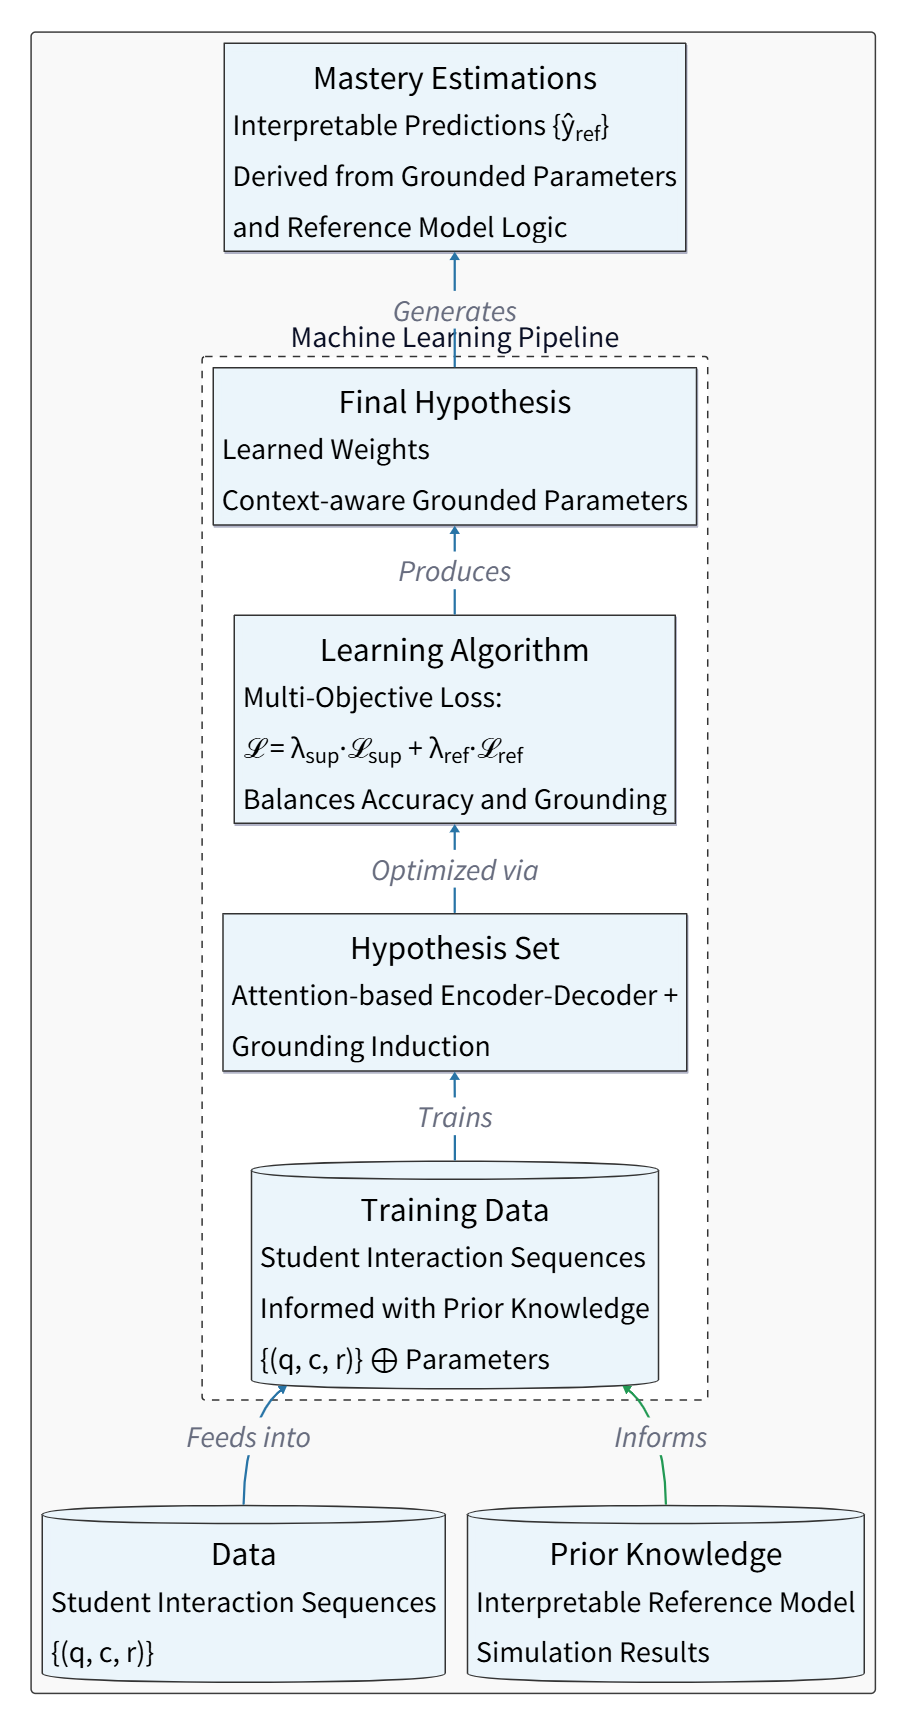
\includegraphics[width=0.45\textwidth]{img/iml.png}
    \caption{\protect\hl{Dimensions} %MDPI: 1. Please DO NOT change any data in figures/tables or replace into new figures/tables during proofreading stage since paper has been accepted
%2. Please recheck all figures and make sure there are no duplicated figures in the whole manuscript. 
 of IML in~gTransformer.}
    \label{fig_info_flow}
\end{figure} %MDPI EE: please revise "Encoder-Decoder" to "Encoder--Decoder" in Figure 1. 
%AuthorsAnswer: We have revised "Encoder-Decoder" to "Encoder--Decoder" in Figure 1.

Within the context of our architecture, the~{operationalisation} of these dimensions can be explained as follows: 

\begin{itemize}
    \item Prior Knowledge: The source of theoretical information comprises simulation results from a reference model, typically expressed as parameter values that represent foundational pedagogical constructs.
    \item Training Data: Empirical student interaction histories are augmented with prior knowledge to train the model.
    \item Hypothesis Set: An attention-based Transformer architecture is employed to provide the inductive biases necessary to lead the model toward desired states.
    \item Learning Algorithm: The model is {optimised} via a multi-objective loss function formulated to balance the trade-off between predictive performance and pedagogical~interpretability.
    \item Final Hypothesis: This comprises a set of learned weights that drive latent representations from which parameter values aligned with the reference model can be extracted. %MDPI EE: please check that the intended meaning has been retained.
    \item Mastery Estimations: The outputs generated through the grounded parameters serve as inputs to the reference model to produce interpretable mastery estimations.
\end{itemize}


\subsection{Architecture}

The gTransformer architecture, illustrated in Figure~\ref{gtransformer_arch}, implements a theory-guided deep learning framework that integrates BKT concepts throughout the processing pipeline. The~architecture is {organised} into six functional layers, which are detailed in the following subsections. Specifically, we: (i) begin with input data comprising student interaction sequences along with prior knowledge from the Bayesian reference model (\mbox{\cref{sec_input}}); (ii)~proceed to explain difficulty-aware embeddings that encode skill-specific variations (\mbox{\cref{sec_embeddings}}); (iii) describe the attention-based encoder--decoder mechanism used to construct {contextualised} latent representations (\cref{sec_enc_dec}); (iv) explain how grounded parameters are obtained by combining theoretical bases with contextual projections (\mbox{\cref{sec_grounded_params}}); (v)~present the output heads intended to generate supervised predictions and interpretable predictions (\cref{sec_output_heads}); and (vi) conclude with the multi-objective loss function that orchestrates the training process to achieve both predictive performance and theory-based interpretability (\cref{sec_loss}).

\subsubsection{Input~Components} \label{sec_input}

{The problem of KT can be formally conceptualised as a supervised sequence modelling task aimed at estimating the longitudinal evolution of student knowledge based on their historical interaction traces. The~input to the system consists of a temporal sequence of student interaction sequences enriched with population-level parameters from a pre-fit BKT reference model. Student interactions are represented as temporal sequences of tuples $(q_t, c_t, r_t)$, where $q_t$ denotes the question identifier, $c_t$ represents the associated knowledge component, concept or skill, and~$r_t \in \{0, 1\}$ indicates the binary correctness of the student's response at timestep $t$.}

{These empirical interaction traces are augmented with theoretical priors extracted from the BKT reference model. For~each knowledge component $c$, we obtain population-level estimates of the four BKT parameters introduced in Section \ref{sec_bkt}: \textit{initial mastery} $P(\text{L}_0)$, \textit{learn rate} $P(\text{T})$, \textit{Guess} probability $P(\text{G})$, and~\textit{Slip} probability $P(\text{S})$. Only $P(\text{L}_0)$ and $P(\text{T})$ undergo the grounding process to calculate the interpretable predictions $\hat{y}_{\text{ref}}$.}

{In contrast the \textit{Guess} and \textit{Slip} parameters are set to fixed, population-level values estimated by the reference BKT model to prioritise the interpretability of knowledge acquisition over the modelling of performance errors. In~the established BKT literature, $P(\text{L}_0)$ and $P(\text{T})$ are considered the primary parameters reflecting a student's latent state, whereas \textit{Guess} and \textit{Slip} are often viewed as performance parameters tied to the assessment item properties~\citep{yudelson2013individualized}. By~fixing the latter, the~model remains focused on the core pedagogical constructs whilst avoiding model degeneracy challenges~\citep{baker2008more} that arise when all four parameters vary simultaneously.} 
\begin{figure}[H]
   % \centering
    
\includegraphics[width=1.0\textwidth]{img/arch.png}
    \caption{\protect\hl{Functional} %MDPI: We moved the figure here to avoid large blank, please confirm.
%MDPI: We revised the hyphen (-) to a minus sign (“−” U+2212). Please confirm.
 layers of the gTransformer architecture. {Grey} denotes standard Transformer elements; blue denotes gTransformer-specific~elements.}
    \label{gtransformer_arch}
\end{figure} %MDPI EE: please revise "Encoder-Decoder" to "Encoder--Decoder" in Figure 2.
\unskip


\subsubsection{Embeddings} \label{sec_embeddings}

For question embeddings, we define
\begin{equation} \label{eq:task_embedding}
    \mathbf{x}'_t = \mathbf{c}_q + u_q \cdot \mathbf{d}_c,
\end{equation}
where $\mathbf{c}_q \in \mathbb{R}^{d}$ represents the invariant concept base embedding (encoding the semantic identity of the knowledge component), $u_q \in \mathbb{R}$ is a scalar difficulty parameter specific to question $q$, and~$\mathbf{d}_c \in \mathbb{R}^{d}$ is the concept-specific difficulty variation axis. This formulation allows multiple questions targeting the same concept to share a common semantic core ($\mathbf{c}_q$) while differing in their position along a learned difficulty direction ($\mathbf{d}_c$), with~the magnitude of displacement controlled by the per-question difficulty scalar ($u_q$).

Similarly, for~interaction history embeddings (encoding both the question and the student's response), we employ
\begin{equation} \label{eq:interaction_embedding}
    \mathbf{y}'_t = \mathbf{e}_{c,r} + u_q \cdot \mathbf{f}_{c,r},
\end{equation}
where $\mathbf{e}_{c,r} \in \mathbb{R}^{d}$ is the interaction base embedding (jointly encoding the concept $c$ and response outcome $r$), and~$\mathbf{f}_{c,r} \in \mathbb{R}^{d}$ is the interaction-specific difficulty variation~axis. 


These embeddings serve as the primary inputs to the Transformer's attention mechanism, providing multidimensional representations that enable attention-driven discovery of relevant {behavioural} patterns across the student's learning~history.

\subsubsection{Attention-Based~Encoders--Decoders} \label{sec_enc_dec}

{The core processing engine of gTransformer is a stacked Transformer architecture composed of $n$ encoder blocks and $2n$ decoder blocks. In~our default configuration ($n=4$), this results in 4 encoder layers and 8 decoder layers, providing a total of 12 sequential attention-driven processing stages. The~architecture does not utilise explicit pooling layers (such \hl{as} %MDPI: Please confirm the special font format if keep. Please check all.
 \texttt{MaxPool} or \texttt{AvgPool}) but rather relies on the attention mechanism to perform dynamic, context-aware aggregation of information across the temporal sequence. The~encoder processes the student's longitudinal interaction history through $n$ sequential self-attention layers, transforming the sequence of interaction embeddings $\{\mathbf{y}'_1, \mathbf{y}'_2, \ldots, \mathbf{y}'_{t-1}\}$ into a tensor of contextualised latent representations. Each encoder block applies multi-head self-attention ($h=4$ or $h=8$ depending on the dataset) with masking to prevent information leakage from future timesteps, followed by a position-wise feed-forward network (FFN) with a hidden dimension of $d_{\text{ff}} = 256$. Within~each block, we apply residual connections followed by Layer Normalization and dropout ($p=0.1$) to ensure numerical stability and prevent over-fitting, following the established Transformer standards~\citep{vaswani2017attention}.}

{The decoder architecture employs an alternating pattern of $2n$ sequential layers. Odd-numbered decoder layers (layers 1, 3, 5, \dots, $2n-1$) perform self-attention over the current question embeddings $\mathbf{x}'_t$ using four or eight heads, allowing the model to examine multiple aspects of the current task without incorporating response history. Even-numbered decoder layers (layers 2, 4, 6, \dots, $2n$) perform cross-attention between the current question representation and the encoder's output, effectively acting as a knowledge retriever that selectively weights relevant evidence from the student's encoded learning trajectory.}

The final decoder layer produces an output tensor $\mathbf{d}_{\text{out}} \in \mathbb{R}^{t \times d}$, which is concatenated with the question embedding to form the high-dimensional context vector
\begin{equation} \label{eq:context_vector}
    \mathbf{z}_t = [\mathbf{d}_{\text{out},t}; \mathbf{x}'_t] \in \mathbb{R}^{z},
\end{equation}
where the dimensionality of $\mathbf{z}_t$ is the combined dimensionality of the decoder output and question embedding space. 
This context vector serves as a comprehensive encoding of the student's current cognitive state, {synthesising} information from both the observed interaction history and the current task~characteristics.

\subsubsection{Grounded~Parameters} \label{sec_grounded_params}

To ensure pedagogical interpretability, gTransformer estimates BKT parameters through an additive composition mechanism operating in logit space. For~each knowledge component $c$, we define theoretical base parameters $\ell_{\text{L}_0,c}$ and $\ell_{\text{T},c}$, {initialised} as the logit-transformed population-level BKT priors:
\begin{equation} \label{eq:theory_base}
    \ell_{\text{L}_0,c} = \operatorname{logit}(P(\text{L}_0)_c), \quad \ell_{\text{T},c} = \operatorname{logit}(P(\text{T})_c).
\end{equation}
\hl{These} %MDPI: Please confirm that the unindented formatting is preserved here. Please check all after equations.
 bases are implemented as scalar embeddings with Gaussian {initialisation} {centred} at the theoretical~values.

Contextual adjustments are computed via dot products between the latent context vector $\mathbf{z}_t$ and learnable semantic axes. For~each concept $c$, we define a knowledge axis $\mathbf{k}_{c} \in \mathbb{R}^{z}$ and a learning velocity axis $\mathbf{v}_{c} \in \mathbb{R}^{z}$. The~contextual projections, representing the student-specific knowledge ($k_s$) and learning velocity ($v_s$), are calculated as
\begin{equation} \label{eq:contextual_projection}
    k_{s,t} = \mathbf{z}_t \cdot \mathbf{k}_c, \quad v_{s,t} = \mathbf{z}_t \cdot \mathbf{v}_c.
\end{equation}
\hl{These} dot products project the high-dimensional latent state onto interpretable semantic dimensions, quantifying how much the student's observed {behaviour} deviates from the population average along the dimensions of initial mastery and learning~velocity.

The final grounded parameters are obtained through additive composition in logit space, followed by sigmoid activation to ensure valid probability bounds:
\begin{equation} \label{eq:grounded_params}
    p_{\text{L}_0,t} = \sigma(\ell_{\text{L}_0,c} + k_{s,t}), \quad p_{\text{T},t} = \sigma(\ell_{\text{T},c} + v_{s,t}).
\end{equation}
\hl{This} design ensures that the model's parameter estimates remain structurally anchored to BKT theory, with~the base terms providing pedagogically sound {initialisation}, while contextual projections enable {individualised} adjustments driven by observed student~{behaviour}.

\subsubsection{Output~Heads} \label{sec_output_heads}

The gTransformer model generates predictions through various output heads, each serving a distinct functional role in the architecture's dual objectives of predictive accuracy and pedagogical~interpretability:
\begin{itemize}
    \item Supervised Prediction Head (\boldmath{$p_{\text{sup}}$}): {A multi-layer perceptron (MLP) directly maps the high-dimensional context vector $\mathbf{z}_t$ to a correctness prediction. The~context vector ($\mathbf{z} \in \mathbb{R}^{128}$) is passed through a sequence of three linear layers with neuron sizes of 512, 256, and~1, respectively. Each hidden layer is followed by a \texttt{ReLU} activation function and a dropout layer ($p=0.1$).} This head is optimised purely for predictive accuracy via binary cross-entropy loss, leveraging the full expressive capacity of the Transformer's learned representations without theoretical constraints.
    \item Interpretable Output Head (\boldmath{$p_{\text{ref}}$}): The grounded BKT parameters $(p_{\text{L}_0,t}, p_{\text{T},t})$ are passed through an implementation of BKT logic, which performs a retrospective belief update walk over the student's interaction history. At~each timestep, the~BKT logic computes the probability of correctness $\hat{y}_{\text{ref},t}$ using the standard BKT update equations with the model's grounded parameters and the fixed population-level \textit{Guess} and \textit{Slip} values. These predictions are intrinsically interpretable because they can be directly tracked to established pedagogical constructs, providing a transparent causal explanation that justifies each estimation through the theoretical lens of BKT. This head ensures that the grounded parameters retain their intended semantic meaning by requiring them to produce valid predictions subjected to the reference model's reasoning process.
    \item Linear Probe Heads: Two dedicated linear layers extract BKT parameter estimates directly from the context vector: $\hat{p}_{\text{L}_0,t} = \sigma(\mathbf{W}_{\text{L}_0} \mathbf{z}_t)$ and $\hat{p}_{\text{T},t} = \sigma(\mathbf{W}_{\text{T}} \mathbf{z}_t)$. Unlike the grounded parameter projections (which use concept-specific semantic axes), these probes are global linear extractors shared across all concepts. They serve to verify that the Transformer's internal representations explicitly encode the targeted pedagogical constructs in a linearly accessible manner.
\end{itemize}

\subsubsection{Multi-Objective~Loss} \label{sec_loss}

The training objective balances predictive performance with pedagogical grounding through a weighted combination of three loss terms:
\begin{equation} \label{eq:total_loss}
    \mathcal{L}_{\text{total}} = \lambda_{\text{sup}} \mathcal{L}_{\text{sup}} + \lambda_{\text{ref}} \mathcal{L}_{\text{ref}} + \lambda_{\text{probe}} \mathcal{L}_{\text{probe}}.
\end{equation}

The supervised loss $\mathcal{L}_{\text{sup}}$ measures the binary cross-entropy between the MLP's direct predictions $\hat{y}_t$ and the ground truth responses $r_t$, driving the model to {maximise} predictive~accuracy:
\begin{equation}
    \mathcal{L}_{\text{sup}} = -\frac{1}{N} \sum_{t=1}^N \left[ r_t \log(\hat{y}_t) + (1-r_t) \log(1-\hat{y}_t) \right].
\end{equation}

The reference loss $\mathcal{L}_{\text{ref}}$ applies the same binary cross-entropy metric to the BKT logic head's predictions $\hat{y}_{\text{ref},t}$, ensuring that the grounded parameters $(p_{\text{L}_0,t}, p_{\text{T},t})$ produce pedagogically meaningful predictions when constrained to operate through BKT's causal inference mechanism:
\begin{equation}
    \mathcal{L}_{\text{ref}} = -\frac{1}{N} \sum_{t=1}^N \left[ r_t \log(\hat{y}_{\text{ref},t}) + (1-r_t) \log(1-\hat{y}_{\text{ref},t}) \right].
\end{equation}

The probing loss $\mathcal{L}_{\text{probe}}$ enforces global alignment between the Transformer's latent representations and BKT constructs by {minimising} the mean squared error between linear probe predictions and population-level BKT targets:
\begin{equation}
    \mathcal{L}_{\text{probe}} = \sum_{k \in \{\text{L}_0, \text{T}\}} \operatorname{MSE}\left( \hat{p}_{k,t}, P(k)_c \right).
\end{equation}

This loss implements a grounding mechanism that constrains the context vector $\mathbf{z}_t$ to align its internal structure such that pedagogical parameters can be extracted via simple linear transformations. By~constraining the latent space globally, rather than merely {regularising} output parameters locally, the~probing loss ensures that interpretability is structurally embedded throughout the model's~representations.

The default configuration uses weight coefficients $\lambda_{\text{sup}} = 1.0$, $\lambda_{\text{ref}} = 0.5$, and \mbox{$\lambda_{\text{probe}} = 1.0$}, balancing supervised performance with theoretical grounding while {prioritising} global latent space alignment through active~probing.

\section{\protect\highlighting{Experimental}%MDPI: 1. In the main text, the companies/manufacturers of chemicals and reagents, devices, instruments, commercial cell lines/samples/materials should be indicated together with their city (states abbreviation is required for USA and Canada) and country in their first appearance;
%2. For all the software used, please state the version number of the software, if it is not applicable, it can be ignored, and the related website or proof should be provided. 
~Setup} \label{sec_experiment}

This section details the experimental setup employed to train and evaluate gTransformer relative to various baseline models. It includes a description of the validation methodology, training setup, datasets (Table \ref{tab_datasets}), and benchmark models selected for comparative evaluation. 

\subsection{Methodology} \label{sec_methodology}
\unskip

\subsubsection{{\protect\highlighting{Performance--Interpretability Trade-Off (RQ1)}}}%MDPI: The heading is repeat with sec5.1, please check.
 \label{sec:rq1_method}

{To quantify the balance between predictive power and transparency, we assess gTransformer using four distinct prediction variants:}
{(1) ablated supervised predictions ($p_{\text{sup}1}$), representing the model's maximum capacity without grounding;}
{(2) grounded supervised predictions ($p_{\text{sup}2}$) from~the standard supervised output;}
{(3) interpretable predictions ($p_{\text{ref}}$), derived exclusively from the BKT logic using grounded parameters; and}
{(4) population-level BKT predictions ($p_{\text{bkt}}$).}


{We establish three key metrics to quantify the trade-off:}
\begin{align}
\mathcal{I}_{\text{drop}} &= p_{\text{sup}1} - p_{\text{sup}2} \label{eq:int_drop} \\
\mathcal{I}_{\text{cost}} &= p_{\text{sup}2} - p_{\text{ref}}   \label{eq:int_cost} \\
\mathcal{I}_{\text{gain}} &= p_{\text{ref}} - p_{\text{bkt}},   \label{eq:int_gain}
\end{align}
where $\mathcal{I}_{\text{drop}}$ (interpretability drop) measures the impact of theoretical constraints on neural capacity, $\mathcal{I}_{\text{cost}}$ (interpretability cost) quantifies the accuracy reduction when switching to interpretable logic, and~$\mathcal{I}_{\text{gain}}$ (interpretability gain) represents the advantage over traditional population-level models.

\subsubsection{{Grounded Interpretability Validation (RQ2)}}

{To verify that gTransformer's internal states are pedagogically valid, we implement a triple-validation methodology based on the following hypotheses:}

\begin{itemize}
\item {\textbf{\hl{H2.1: Structural Alignment}%MDPI: Please confirm that the hypotheses format is preserved.
}: Latent representations in the gTransformer model are structurally organised around Bayesian concepts (initial mastery $P(\text{L}_0)$ and learn rate $P(\text{T})$) as the dominant organising principle. This is verified using \textit{diagnostic probing}~\citep{hewitt2019designing, belinkov2022probing}. We measure \textit{fidelity} as the quality of the parameter recovery via the coefficient of determination $R^2$ and Pearson correlation $r$. To~distinguish genuine structural encoding from spurious correlations, \textit{selectivity} is defined as}
\begin{equation} \label{eq:selectivity}
    \Delta R^2 = R^2_{\text{target}} - R^2_{\text{control}},
    \end{equation}
where $R^2_{\text{target}}$ represents the probe performance on true BKT targets and $R^2_{\text{control}}$ is the performance on a control task with randomly shuffled targets.
    \item H2.2: Semantic Alignment: Grounded parameters must retain their pedagogical semantics. We evaluate the monotonic consistency (Spearman correlation $\rho$) between the model's grounded parameters and the original theoretical priors to verify pedagogical integrity across datasets.
    \item H2.3: Functional Alignment: \textls[-15]{Quantifies the confidence with which interpretable, theory-constrained estimations ($p_{\text{ref}}$) can substitute for the black-box supervised baseline ($p_{\text{sup}2}$) without significant performance loss. To~quantify this trustworthiness, we define a \textit{composite confidence metric} calculated as a weighted sum of three relevant~dimensions:}
\begin{equation} \label{eq:confidence}
    \operatorname{Confidence} = w_1 \cdot C_{\text{calibrated}} + w_2 \cdot C_{\text{directional}} + w_3 \cdot C_{\text{percentile}},
    \end{equation}
where $w_1$, $w_2$, and $w_3$ are relative weights. These dimensions include numerical proximity ($C_{\text{calibrated}}$), binary decision agreement ($C_{\text{directional}}$), and~a dataset-wide rank of prediction disagreement ($C_{\text{percentile}}$).
\end{itemize}


\subsubsection{\texorpdfstring{{\protect\highlighting{Context-Aware Personalisation (RQ3)}}}{Context-Aware Personalisation (RQ3)}} %MDPI: The heading is repeat with sec5.3, please check.
 \label{sec:rq3_method}

{To evaluate the model's ability to provide context-aware predictions, we implement an approach that clusters students along two dimensions corresponding to the predicted parameter values: prior knowledge ($p_{\text{L}_0}$) and learn rate ($p_{\text{T}}$). We select students with identical responses to the same sequence of questions but belonging to different clusters (i.e., demonstrating different longitudinal learning patterns). We then illustrate how gTransformer customises predictions based on these diverse learning contexts, whereas traditional BKT models, being fundamentally Markovian, produce identical predictions for the same response sequence regardless of the historical learning context. This approach highlights the non-Markovian patterns and context-aware personalisation that population-level baselines fundamentally cannot represent.}

\subsection{Training~Setup}

The gTransformer model was implemented in \texttt{PyTorch} using the \texttt{pyKT} library~\citep{liu2022pykt} for {standardised} data preprocessing, dataset splitting, and~baseline model implementation. Training and evaluation followed a standard five-fold cross-validation protocol using an 80/20 train/test split. Predictive performance was measured using Area Under the Curve (AUC), applying the question-level mean late-fusion protocol as recommended in~\cite{liu2022pykt}. Hyperparameter configurations for benchmark models were aligned with the {optimised} values reported in the official \texttt{pyKT} repository. The~specific configurations used for gTransformer are detailed in \cref{tab:params}. {All experiments were conducted utilising 24 CPU cores and 5 NVIDIA Tesla GPUs.} For~the Bayesian Knowledge Tracing baseline, we utilised \textit{pyBKT}~\citep{badrinath2021pybkt}, a Python implementation of the algorithm that estimates student cognitive mastery from problem-solving sequences.
%AuthorsAnswer: Added reference to the pyBKT library as requested, which was used for the BKT baseline implementation.


\begin{table}[H]
\centering
\small
\caption{Hyperparameter configurations for performance benchmark (\protect\hl{Table} %MDPI: The first citation of each table should appear in numerical order. Citations of Table 3 and 4 are before Table 2, please revise and ensure that the first citation of each table appears in numerical order. This is very important to revise, otherwise, it may affect publication process.
 \ref{tab_performance}) and trade-off evaluation (\protect\hl{Table} \ref{tab:tradeoff}).}
\label{tab:params}
\begin{tabularx}{\textwidth}{LCC}
\toprule
\textbf{Hyperparameter} & \textbf{Performance} & \textbf{Trade-Off} \\
\midrule
\multicolumn{3}{l}{\textit{\hl{Ablation Configuration}%MDPI: Please add an explanation for the use of italics in the table footer. If the italics is unnecessary, please remove it. 
}} \\
Ablation mode & \hl{\texttt{all}} %MDPI: Please confirm if the font formatting is necessary; if not, please remove it. The following are the same.
 & \texttt{none} \\
$\lambda_{\text{sup}}$ & 1.0 & 1.0 \\
$\lambda_{\text{ref}}$ & 0 & 0.5 \\
$\lambda_{\text{probe}}$ & 0 & 1.0 \\
\midrule
\multicolumn{3}{l}{Architecture Configuration} \\
$d_{\text{model}}$ & 64 & 64 \\
{$n_{\text{blocks}}$ (Encoder/Decoder)} & 4/8 & 4/8 \\
{Total attention layers} & {12} & {12} \\
$d_{\text{ff}}$ & 256 & 256 \\
Attention heads & 4 & \makecell{AS2009: 8\\others: 4} \\
{Output MLP dimensions} & {[128, 512, 256, 1]} & {[128, 512, 256, 1]} \\
{Activation function} & {\texttt{ReLU}} & {\texttt{ReLU}} \\
{Normalization} & {\textit{LayerNorm}} & {\textit{LayerNorm}} \\
\midrule
\multicolumn{3}{l}{Training Configuration} \\
Learning rate & \makecell{NIPS34: $3 \times 10^{-4}$\\others: $10^{-4}$} & $10^{-4}$ \\
Batch size & 64 & 64 \\
{Optimiser} & \texttt{adam} & \texttt{adam} \\
Epochs & 200 & 200 \\
{Dropout ($p$)} & 0.1 & 0.1 \\
{Weight initialization} & \makecell{{Xavier/} \\ {Orthogonal}} & \makecell{{Xavier/} \\ {Orthogonal}} \\
\bottomrule
\end{tabularx}
\end{table}
\unskip


\subsection{Datasets}\label{sec_dataset}

{For our analysis, we utilised the datasets for which the \textit{pyKT} library~\citep{liu2022pykt} provides standardised preprocessing mechanisms, thereby ensuring a rigorous and consistent treatment of student interactions. From~this collection, we excluded the datasets that lack explicit mapping to knowledge components (\textit{Statics2011} and \textit{POJ}), as~this information is essential for pedagogical interpretability, allowing mastery estimations to be anchored to defined educational concepts. The~five datasets selected for this study are described below:}
 
\begin{itemize}
    \item ASSISTments 2009 (AS2009): Collected from the ASSISTments platform during the 2009--2010 school year, this dataset consists of math exercises and has served as the de facto standard benchmark for KT research for the past decade~\citep{feng2009addressing}.
    \item ASSISTments 2015 (AS2015): A larger release from the same platform for~the 2015 school year, this dataset contains the highest number of students among the ASSISTments datasets. It focuses on a specific set of 100 knowledge concepts~\citep{feng2009addressing}.
    \item Algebra 2005 (AL2005): Released as part of the KDD Cup 2010 EDM Challenge, it contains responses from 13--14-year-old students solving Algebra problems~\citep{stamper2010algebra}.
    \item Bridge to Algebra 2006 (BDG2006): Also from the KDD Cup 2010 Challenge, this dataset focuses on the \textit{Bridge to Algebra} tutoring system and includes a high number of total interactions~\citep{stamper2010algebra}.
    \item NeurIPS 2020 Education Challenge (NIPS34): This is a more recent dataset from the Eedi platform containing student answers to multiple-choice math questions, {characterised by subject trees} used for concept mapping~\citep{wang2020instructions}.
\end{itemize}

The characteristics of the datasets are {summarised} in Table~\ref{tab_datasets}.

\begin{table}[H]
\centering
\caption{Characteristics of the benchmark datasets used to evaluate AUC. $N_{\text{s}}$, $N_{\text{c}}$, $N_{\text{q}}$ and $N_{\text{i}}$ denote the total number of sequences (students), knowledge components, questions and student--item interactions, respectively. \label{tab_datasets}}
\begin{tabularx}{\textwidth}{Lcccc}
\toprule
\textbf{Dataset} & \textbf{Sequences (\boldmath{$N_{\text{s}}$})} & \textbf{Concepts (\boldmath{$N_{\text{c}}$})} & \textbf{Questions (\boldmath{$N_{\text{q}}$})} & \textbf{Interactions (\boldmath{$N_{\text{i}}$})} \\
\midrule
AS2009 & 4217 & 123 & 26,688 & 346,860 \\
AS2015 & 19,917 & 100 & --- & 708,631 \\
AL2005 & 574 & 112 & 210,710 & 809,694 \\
BDG2006 & 1146 & 493 & 207,856 & 3,679,199 \\
NIPS34 & 4918 & 57 & 948 & 1,382,727 \\
\bottomrule
\end{tabularx}
\end{table}
\unskip



\subsection{Baseline~Models}\label{sec_models}

For the comparative analysis, we selected six models that are among the most frequently mentioned baselines~\citep{liu2022pykt}: DKT~\citep{piech2015deep}, DKVMN~\citep{zhang2017dynamic}, SAKT~\citep{pandey2019self}, SAINT~\citep{choi2020towards}, AKT~\citep{ghosh2020context} and ATKT~\citep{GuoHZTL21}. These models represent a representative selection of the recurrent (DKT), memory-augmented (DKVMN), adversarial (ATKT), and~attention-based (SAKT, SAINT, and AKT) paradigms, providing a robust and diverse benchmark for evaluating our~model.


\section{Results and~Discussion} \label{sec_results}
\unskip

\subsection{\texorpdfstring{\protect\highlighting{Performance--Interpretability Trade-Off (RQ1)}}{Performance--Interpretability Trade-Off (RQ1)}} \label{sec_tradeoff}

To evaluate the predictive performance of gTransformer, we {utilise} the Area Under the Curve (AUC) across the benchmark datasets described in \cref{sec_dataset}. The~experimental results are {summarised} in Table~\ref{tab_performance}.

\begin{table}[H]
\centering
\caption{Comparison of predictive performance across various benchmark datasets. The~table reports AUC values for gTransformer and baseline models evaluated at the question level, following a mean late-fusion protocol. Values in bold indicate the best-performing model for each~dataset. \label{tab_performance}}
\begin{tabularx}{\textwidth}{LcCcCc}
\toprule
\textbf{Model} & \textbf{AS2009} & \textbf{AS2015} & \textbf{AL2005} & \textbf{BDG2006} & \textbf{NIPS34} \\
\midrule
AKT & 0.7825 & 0.7081 & \textbf{0.8306} & \textbf{0.8208} & \textbf{0.8033} \\
ATKT & 0.7715 & \textbf{0.7810} & 0.7995 & 0.7889 & 0.7665 \\
DKT & 0.7528 & 0.7031 & 0.8149 & 0.8015 & 0.7689 \\
DKVMN & 0.7440 & 0.7013 & 0.8054 & 0.7983 & 0.7673 \\
SAKT & 0.7263 & 0.6947 & 0.7880 & 0.7740 & 0.7517 \\
SAINT & 0.6921 & 0.6836 & 0.7775 & 0.7781 & 0.7873 \\
\midrule
gTransformer & \textbf{0.7831} & 0.7078 & 0.8240 & 0.8148 & 0.8006 \\
\bottomrule
\end{tabularx}

\end{table}

Compared to baseline models, gTransformer achieves highly competitive performance across all benchmarks. To~ensure a fair comparison with these non-interpretable baselines, we evaluate gTransformer in an ablated configuration ($\lambda_{\text{sup}} = 1.0,~\lambda_{\text{ref}} = 0,~\lambda_{\text{probe}} = 0$). This approach establishes the model's maximum predictive capacity in the absence of theoretical constraints, allowing for a direct assessment against other deep learning architectures. On~AS2009, gTransformer achieves an AUC of 0.7831, outperforming all other evaluated models. It ranks second on AL2005, BDG2006 and NIPS34 (surpassed only by AKT) and~third on AS2015 (behind ATKT and AKT). 

To evaluate the performance trade-off, we compare the results of the ablated configuration ($p_{\text{sup}1}$), the~grounded supervised output ($p_{\text{sup}2}$), the~interpretable predictions ($p_{\text{ref}}$) and the BKT baseline ($p_{\text{bkt}}$). Binary cross-entropy metrics ($p_{\text{bkt}}$) are omitted for AS2015 because this dataset lacks the question-level identifiers required for evaluation. \Cref{tab:tradeoff} presents the results for these evaluations, quantifying the interpretability drop, cost, and~gain as defined in \cref{sec_methodology}. 


\begin{table}[H]
\centering
\small
\caption{AUC--interpretability trade-offs in gTransformer across datasets. The~table shows AUC scores for the predictions of the ablated configuration ($p_{\text{sup}1}$), predictions of the grounded configuration ($p_{\text{sup}2}$), interpretable predictions ($p_{\text{ref}}$) and classical BKT predictions ($p_{\text{bkt}}$). The~$\mathcal{I}_{\text{drop}}$ column shows the cost of grounding ($p_{\text{sup}1} - p_{\text{sup}2}$) and $\mathcal{I}_{\text{cost}}$ shows the interpretability cost ($p_{\text{sup}2} - p_{\text{ref}}$), while $\mathcal{I}_{\text{gain}}$ shows the interpretability gain ($p_{\text{ref}} - p_{\text{bkt}}$).}
\label{tab:tradeoff}
\begin{tabularx}{\textwidth}{LcCccccc}
\toprule
\textbf{Dataset} & \boldmath{$p_{\textbf{sup}1}$} & \boldmath{$p_{\textbf{sup}2}$} & \boldmath{$p_{\textbf{ref}}$} & \boldmath{$p_{\textbf{bkt}}$} & \boldmath{$\mathcal{I}_{\textbf{drop}}$} \textbf{(\%)} & \boldmath{$\mathcal{I}_{\textbf{cost}}$} \textbf{(\%)} & \boldmath{$\mathcal{I}_{\textbf{gain}}$} \textbf{(\%)} \\
\midrule
AS2009 & 0.7831 & 0.7814 & 0.7436 & 0.6097 & 0.0017 (0.2\%) & 0.0378 (4.8\%) & 0.1339 (22.0\%) \\
AS2015 & 0.7078 & 0.7070 & 0.6940 & --- & 0.0008 (0.1\%) & 0.0130 (1.8\%) & --- \\
AL2005 & 0.8240 & 0.8237 & 0.7800 & 0.7215 & 0.0003 (0.0\%) & 0.0437 (5.3\%) & 0.0585 (8.1\%) \\
BDG2006 & 0.8148 & 0.8107 & 0.7810 & 0.6756 & 0.0041 (0.5\%) & 0.0297 (3.6\%) & 0.1054 (15.6\%) \\
NIPS34 & 0.8006 & 0.7987 & 0.7666 & 0.5729 & 0.0019 (0.2\%) & 0.0321 (4.0\%) & 0.1937 (33.8\%) \\
\midrule
\hl{Mean}%MDPI: Please add an explanation for the use of bold in the table footer. If the bold is unnecessary, please remove it.
%AuthorsAnswer: This bold is unnecessary so we remove it. 
 & 0.7861 & 0.7843 & 0.7530 & 0.6449 & 0.0018 (0.2\%) & 0.0313 (3.9\%) & 0.1229 (19.9\%) \\
\bottomrule
\end{tabularx}
\end{table}


The results reveal two insights regarding the accuracy--interpretability trade-off:

\begin{itemize}
    \item Low Cost of Interpretability. This cost can be {analysed} through two distinct metrics. The~interpretability drop ($\mathcal{I}_{\text{drop}}$) measures the impact of grounding constraints ($\mathcal{L}_{\text{ref}}$ and $\mathcal{L}_{\text{probe}}$) on the Transformer's original representational capacity. The~results in Table~\ref{tab:tradeoff} show that this drop is negligible, with~an average of only 0.0018 AUC points (0.2\%), demonstrating that the model {internalises} pedagogical theory without sacrificing its expressive power. The~interpretability cost ($\mathcal{I}_{\text{cost}}$) measures the performance impact of constraining final predictions to the causal logic of the reference model. The~results show that the average cost across datasets is 0.0313 AUC points (3.9\% reduction), which is highly acceptable given the substantial gains in~interpretability.
    
    \item General Interpretability Gain. Comparing $p_{\text{ref}}$ against $p_{\text{bkt}}$ provides a measure of the \textit{interpretability gain} ($\mathcal{I}_{\text{gain}}$). In~all comparable datasets, interpretable gTransformer predictions consistently outperform classical BKT with an average improvement of 0.1229 AUC points (19.9\%), showing a general advantage over population-level priors. 
\end{itemize}

In summary, the~cost of interpretability is consistently low and highly acceptable for practical educational applications. By~accurately recovering student-specific learning parameters, gTransformer bridges the gap between black-box performance and theoretical rigor, offering a superior diagnostic alternative to traditional symbolic approaches without sacrificing~performance.


\subsection{Grounded Interpretability (RQ2)} \label{sec_grounded}

For the remainder of this study, we employ AS2009 as our reference dataset. Given its status as a widely used benchmark and its rich interaction data, it provides an ideal testbed for validating structural and semantic alignment, especially considering the high predictive AUC that gTransformer achieves on this~data.

\subsubsection{Structural Alignment via Diagnostic Probing (H2.1)} \label{sec_structural_alignment}

The H2.1 objective is to demonstrate that grounding constraints actively shape the model's internal structure, rather than merely correlating with outputs. To~verify whether gTransformer's latent representations genuinely {internalise} pedagogical concepts, we analyse the quality of the parameter recovery from the final hidden states $\mathbf{z}_t$. 

\Cref{fig_structural_fidelity_l0,fig_structural_fidelity_t} present the diagnostic probing results via parity plots, comparing BKT theoretical priors (x-axis) with probe-extracted parameters (y-axis). Each point represents an aggregate of interactions, with~its size proportional to the sample density. The~high adherence to the diagonal confirms a high degree of linear recoverability, with~the obtained values indicating strong structural encoding:


\begin{itemize}
    \item \textls[-25]{Initial Mastery $P(\text{L}_0)$: Achieves fidelity $R^2 = 0.549 \pm 0.064$ with Pearson \mbox{$r = 0.743 \pm 0.041$},} indicating strong linear recoverability. The~selectivity $\Delta R^2 = 0.619 \pm 0.061$ exceeds the threshold of 0.5, demonstrating that this is a dominant {organising} principle in the latent space rather than an incidental pattern. The~control task yields a negative $R^2 = -0.069$ (indicating performance worse than a mean-based baseline), confirming that probes cannot recover shuffled~targets.
    
    \item \textls[-15]{Learn Rate $P(\text{T})$: Shows strong structural encoding with fidelity \mbox{$R^2 = 0.515 \pm 0.080$}} and Pearson $r = 0.721 \pm 0.050$. The~selectivity reaches $\Delta R^2 = 0.570 \pm 0.080$, demonstrating robust encoding of learn rate dynamics, with~control $R^2 = -0.055$.
\end{itemize}

\textls[-15]{\textbf{Interpretation}: The high selectivity ($>$0.5) for both parameters validates the H2.1 (structural alignment) hypothesis: BKT constructs are preserved through all Transformer layers and remain as primary organising concepts in final representations used for~prediction.} 

\begin{figure}[H]
%\centering
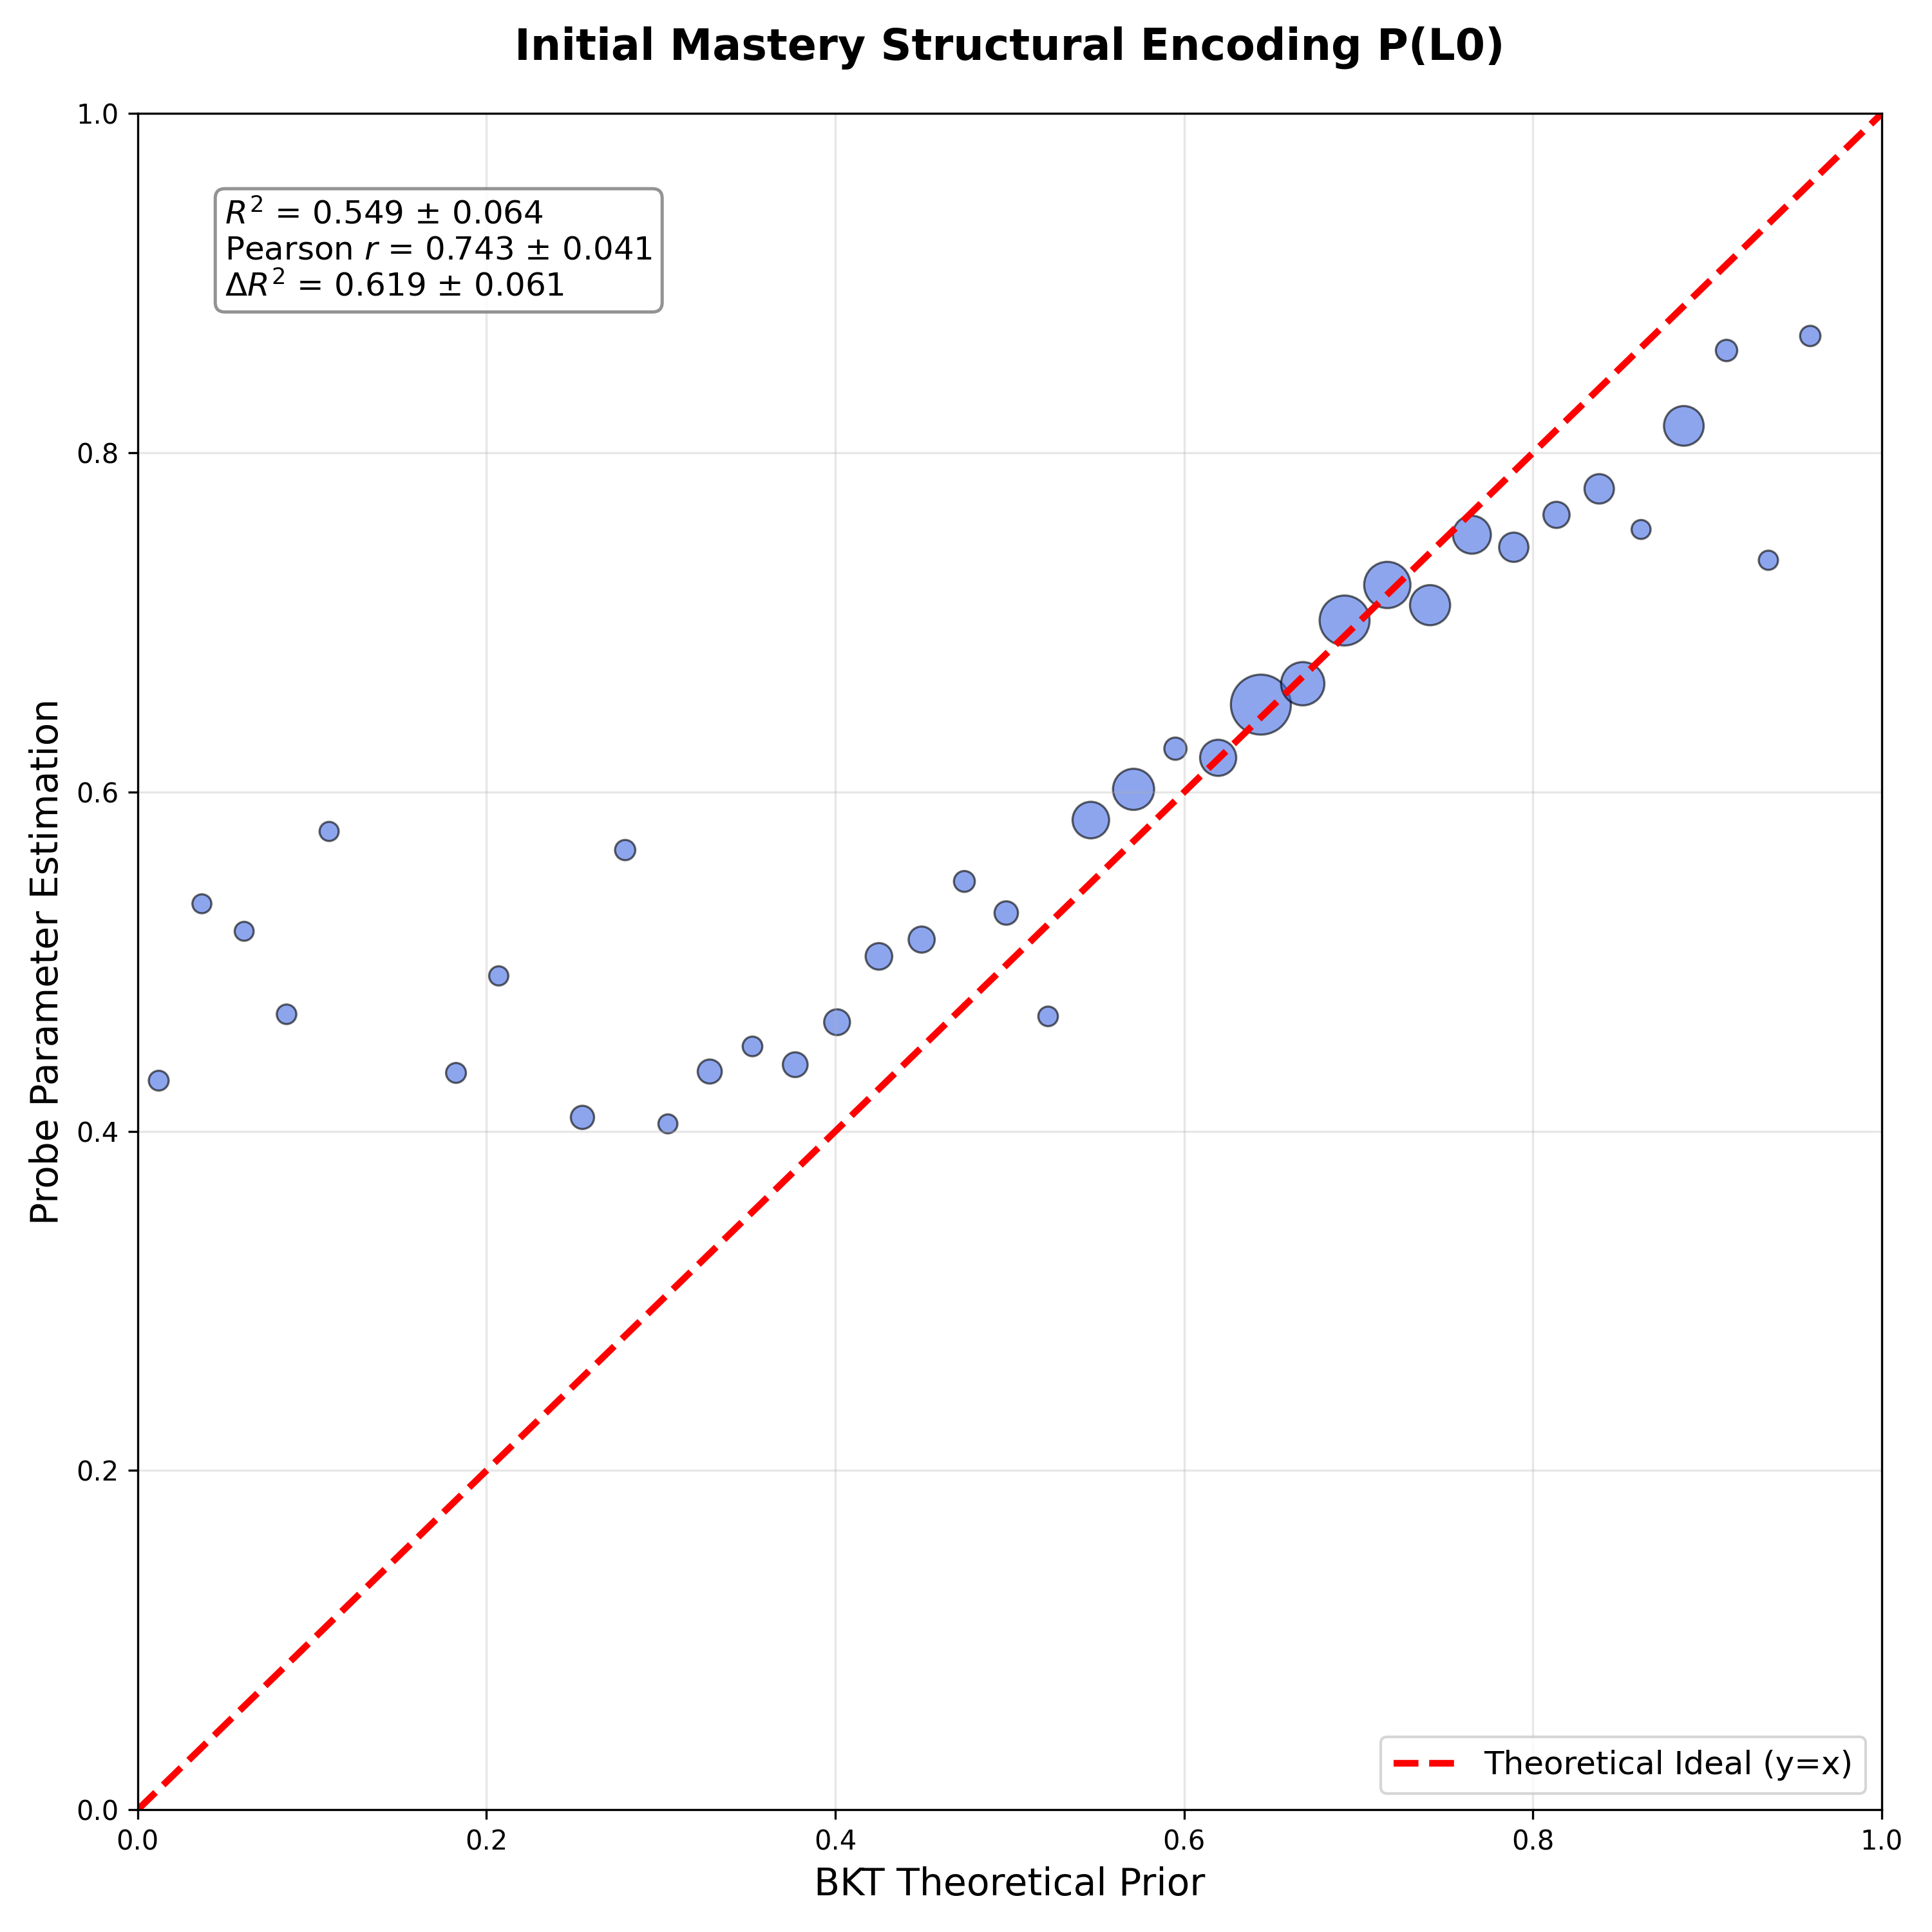
\includegraphics[width=0.70\textwidth]{img/h12_recovery_l0_probe_893468.png}
\caption{\protect\hl{Structural} fidelity for Initial Mastery $P(\text{L}_0)$. Plot demonstrating strong linear recoverability ($R^2=0.549$, $r=0.743$, $\Delta R^2=0.619$) between BKT theoretical priors and probe-extracted parameters. Each bubble represents a binned aggregate of test interactions, with~size encoding sample density. The~high adherence to the diagonal and high selectivity ($\Delta R^2>0.5$) validate that this is a dominant {organising} principle in latent~representations. \label{fig_structural_fidelity_l0}}
\end{figure}
\begin{figure}[H]
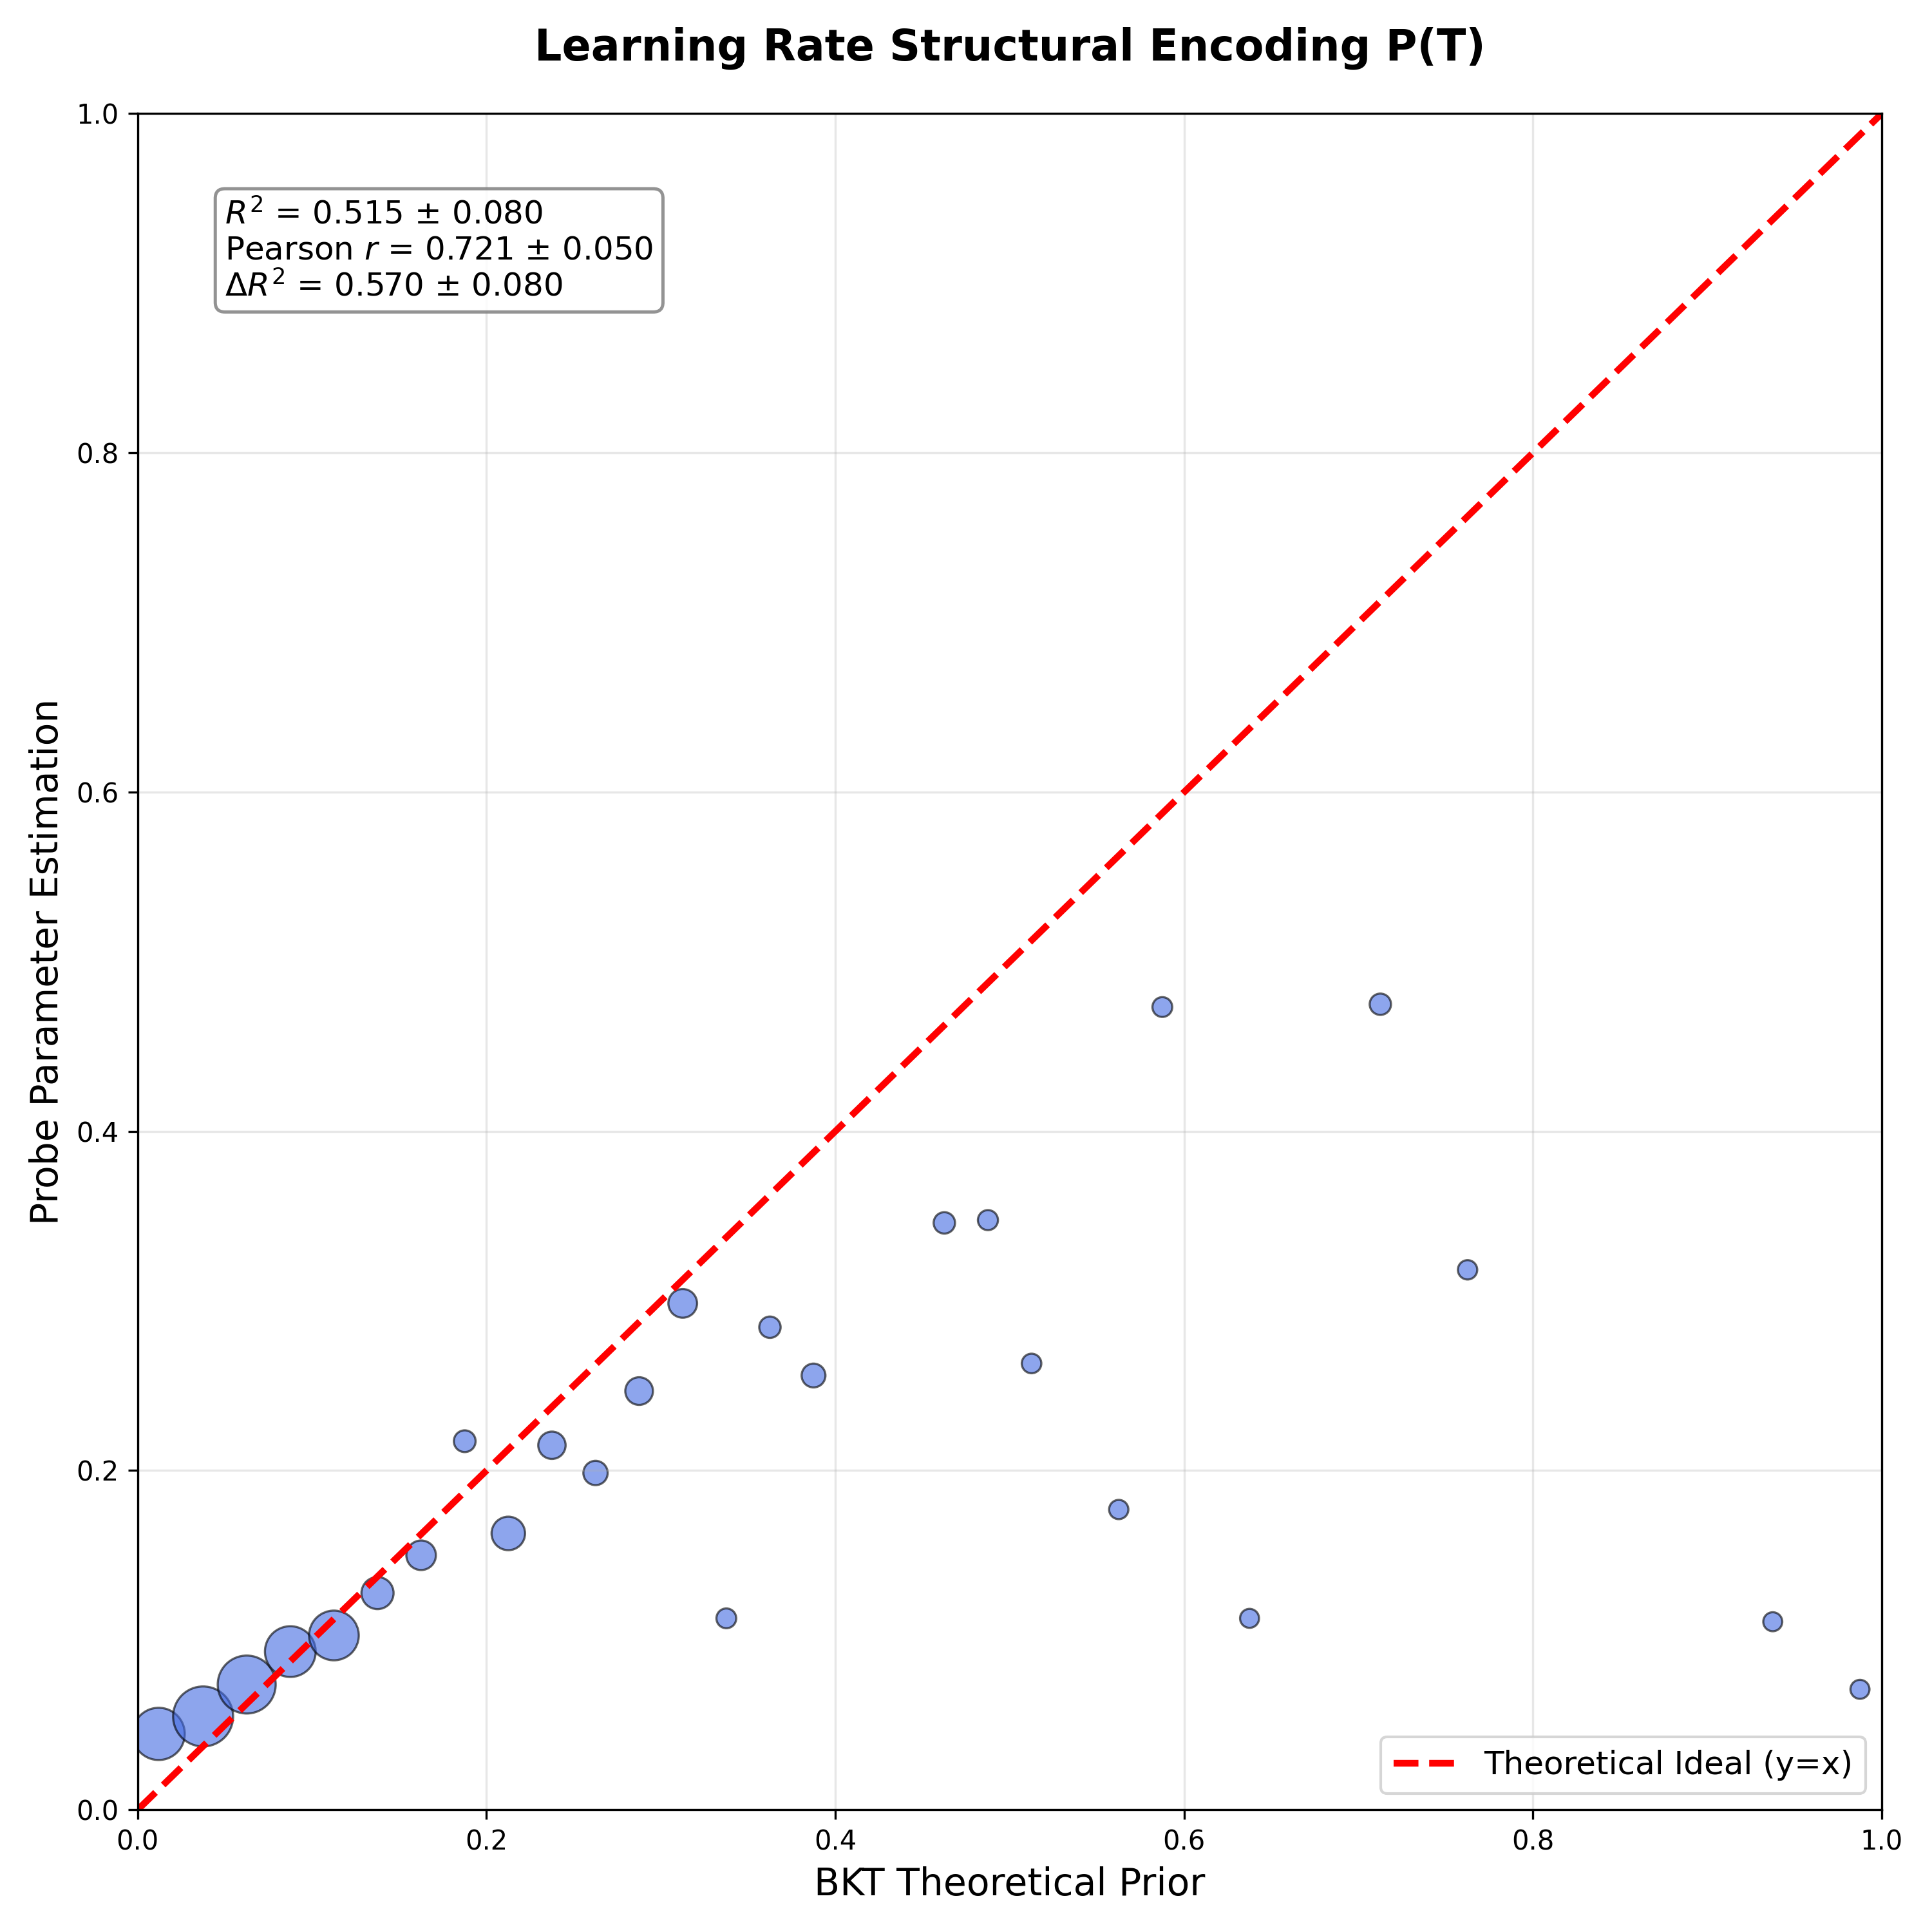
\includegraphics[width=0.70\textwidth]{img/h12_recovery_t_probe_893468.png}
\caption{\protect\hl{Structural}  %MDPI: Please confirm whether the bubble needs an explanation. 
 fidelity for learn rate $P(\text{T})$. Plot demonstrating robust linear recoverability ($R^2=0.515$, $r=0.721$, $\Delta R^2=0.570$) between BKT theoretical priors and probe-extracted parameters. The~high adherence to the diagonal and high selectivity ($\Delta R^2>0.5$) confirm that learn rate dynamics are dominantly encoded in latent~representations. \label{fig_structural_fidelity_t}}
\end{figure}
\unskip

\subsubsection{Semantic Alignment (H2.2)} \label{sec_semantic_alignment}

Hypothesis H2.2 examines whether grounded parameters retain their pedagogical semantics after processing, ensuring models do not repurpose theoretical constructs for black-box {optimisation}. Unlike H2.1, which probes latent representations, H2.2 validates monotonic relationship preservation in final projected parameters. We use Spearman's rank correlation ($\rho$) to measure alignment, as~it captures monotonic consistency without assuming linearity ($\rho \geq 0.6$ strong, $0.4 \leq \rho < 0.6$ moderate).

\Cref{fig_semantic_alignment_l0,fig_semantic_alignment_t} present parity plots comparing BKT theoretical priors (x-axis) with grounded parameters (y-axis), where each bubble represents an aggregate of test interactions with size encoding sample density. The~patterns reveal that:

\begin{itemize}
    \item Initial Mastery ($P_{\text{L}_0}$) shows weak alignment ($\rho = 0.360$) with substantial scatter, indicating strong student-specific {individualisation}. However, MAE = $0.168$ validates that refinements remain within pedagogical bounds, indicating that the model neither abandons nor mechanically reproduces theoretical priors.
    \item Learn Rate ($P_{\text{T}}$) demonstrates moderate alignment ($\rho = 0.544$). A~low MAE = $0.092$ confirms that the model preserves pedagogical understanding of practice effects while enabling context-aware refinement.
\end{itemize}

These findings support that grounded parameters maintain meaningful monotonic alignment with theory while capturing individual heterogeneity. The~differential alignment reveals that learn rates preserve more theoretical structure while initial mastery estimates undergo stronger~individualisation.


\begin{figure}[H]
%\centering
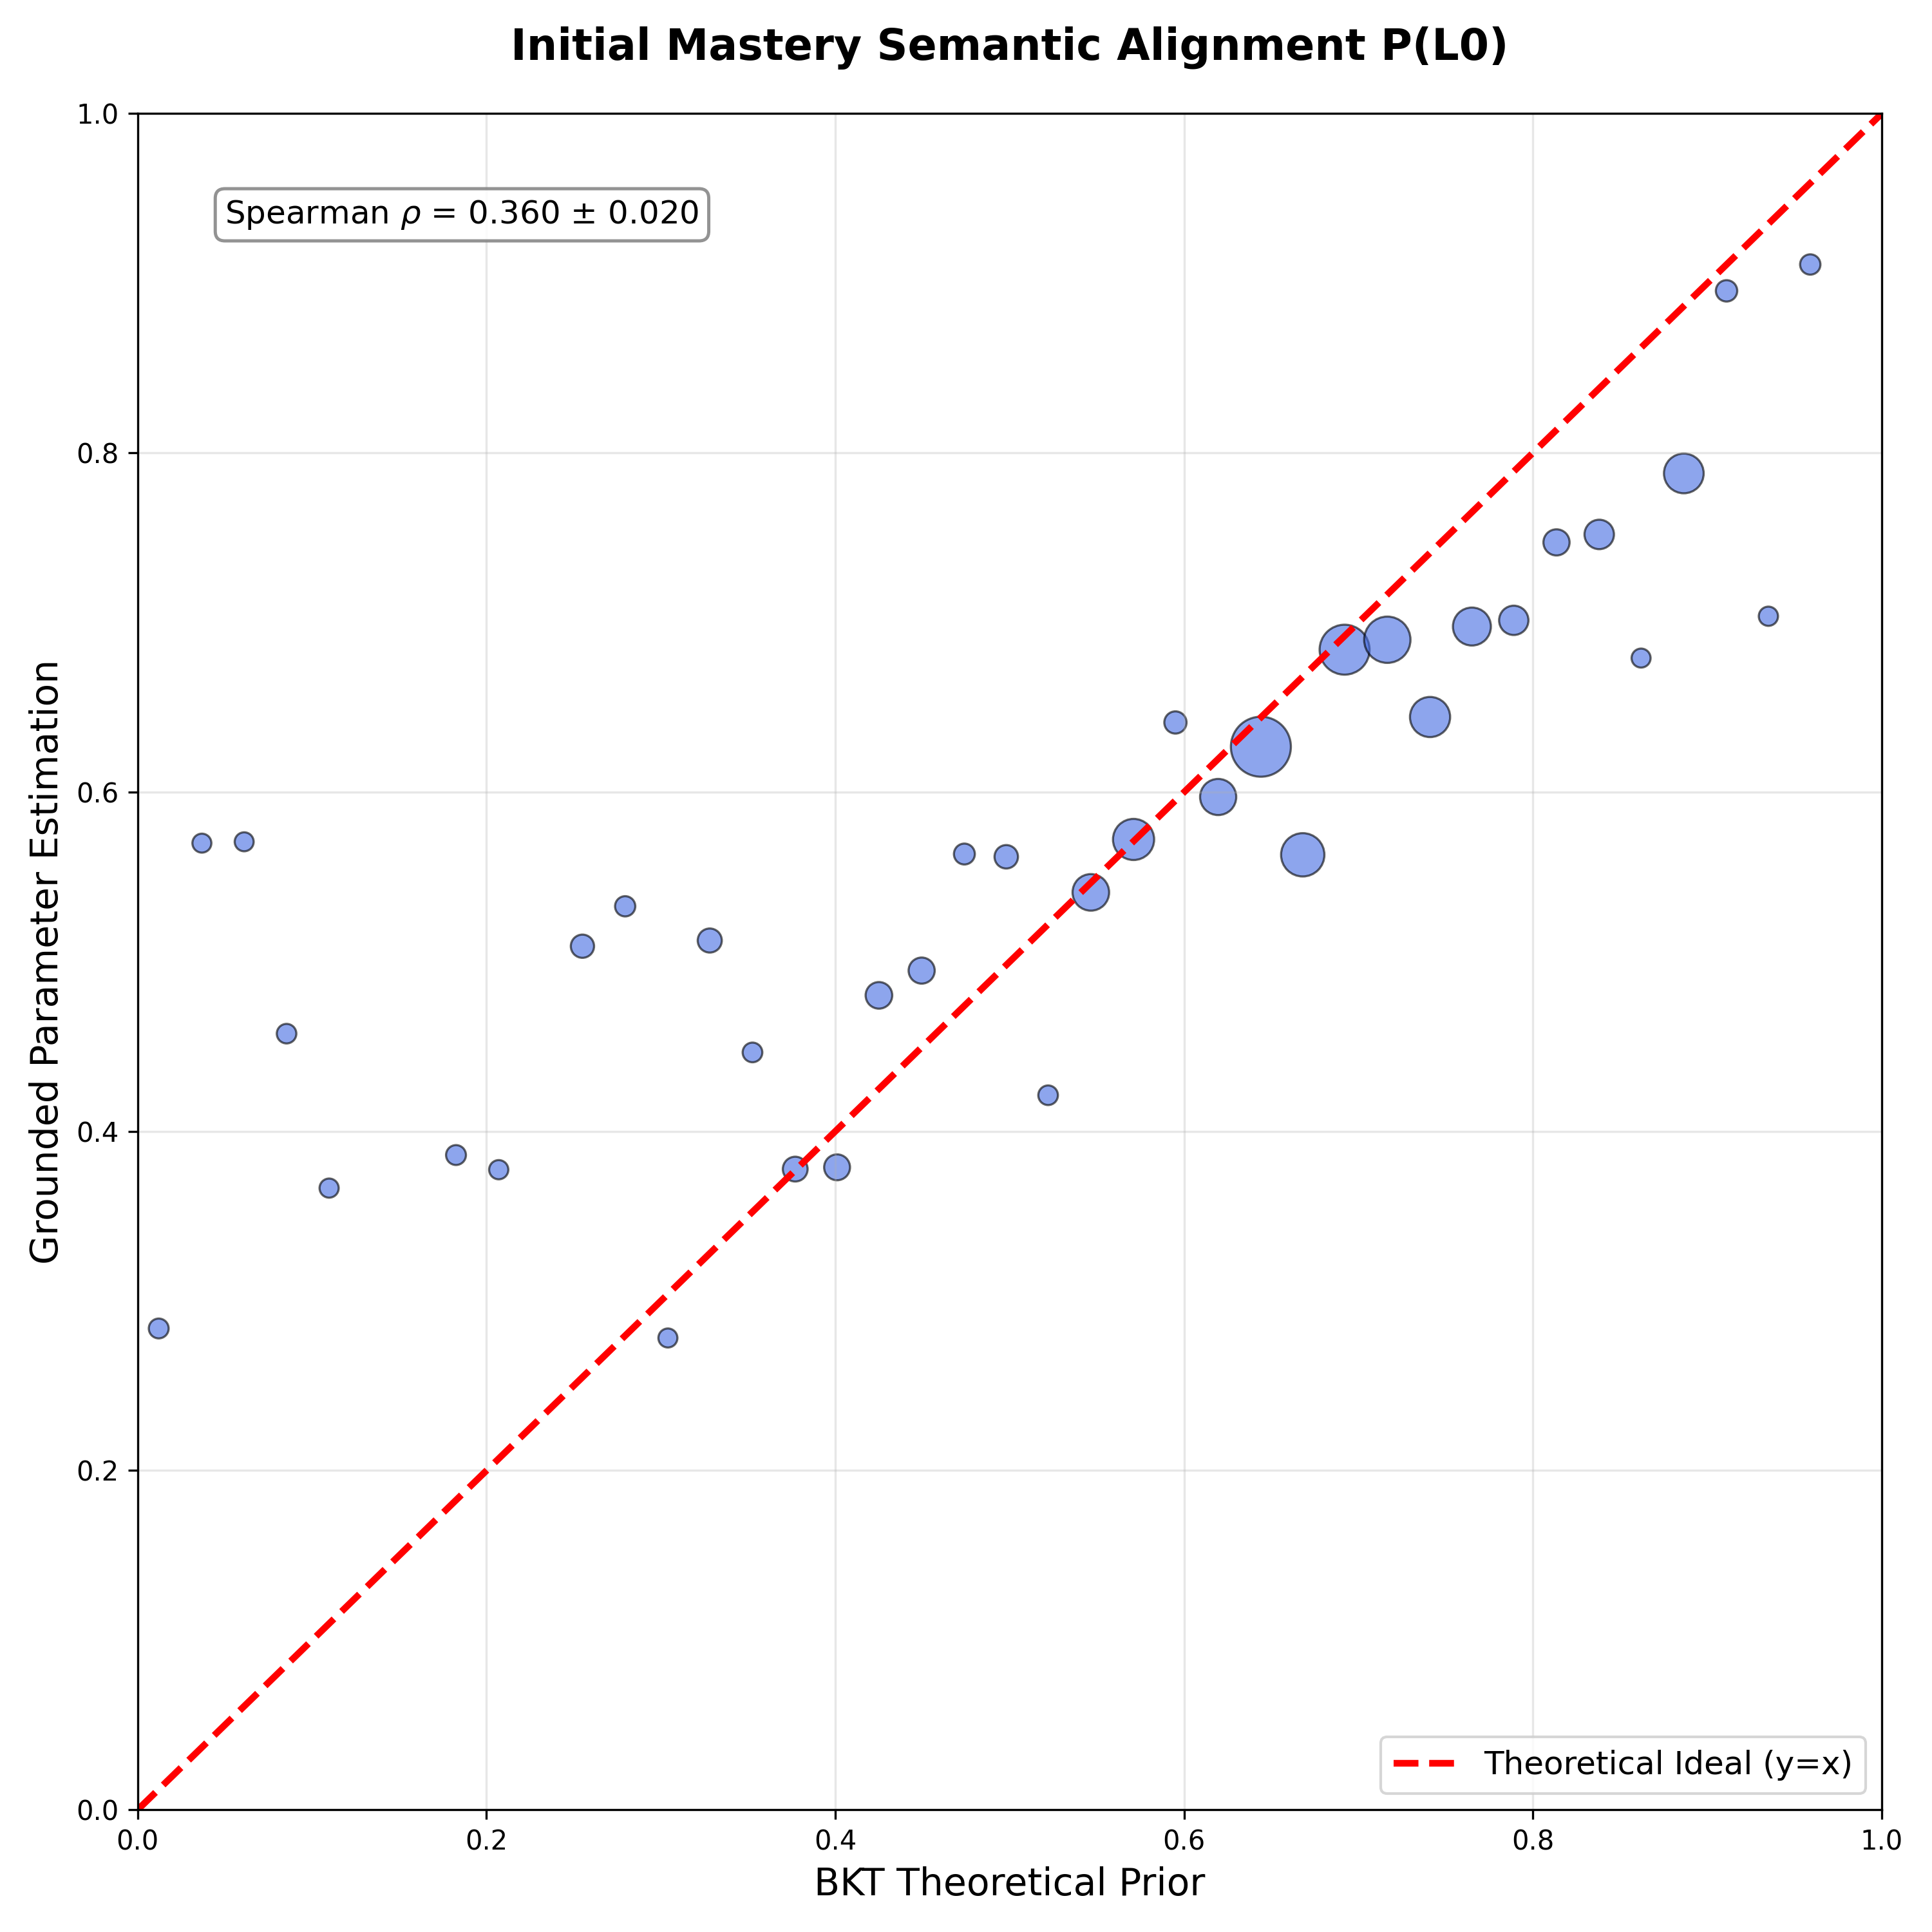
\includegraphics[width=0.68\textwidth]{img/h12_recovery_l0_grounded_893468.png}
\caption{\protect\hl{Semantic} alignment for Initial Mastery $P(\text{L}_0)$. Plot showing weak monotonic relationship preservation (Spearman $\rho = 0.360$, MAE = $0.168$) between BKT theoretical priors and grounded parameters after neural transformation. Each bubble represents an aggregate of test interactions, with~size encoding sample density. The~substantial scatter indicates strong student-specific {individualisation}, with~the model {prioritising} context-aware adaptation over strict adherence to population~priors. \label{fig_semantic_alignment_l0}}
\vspace{12pt}
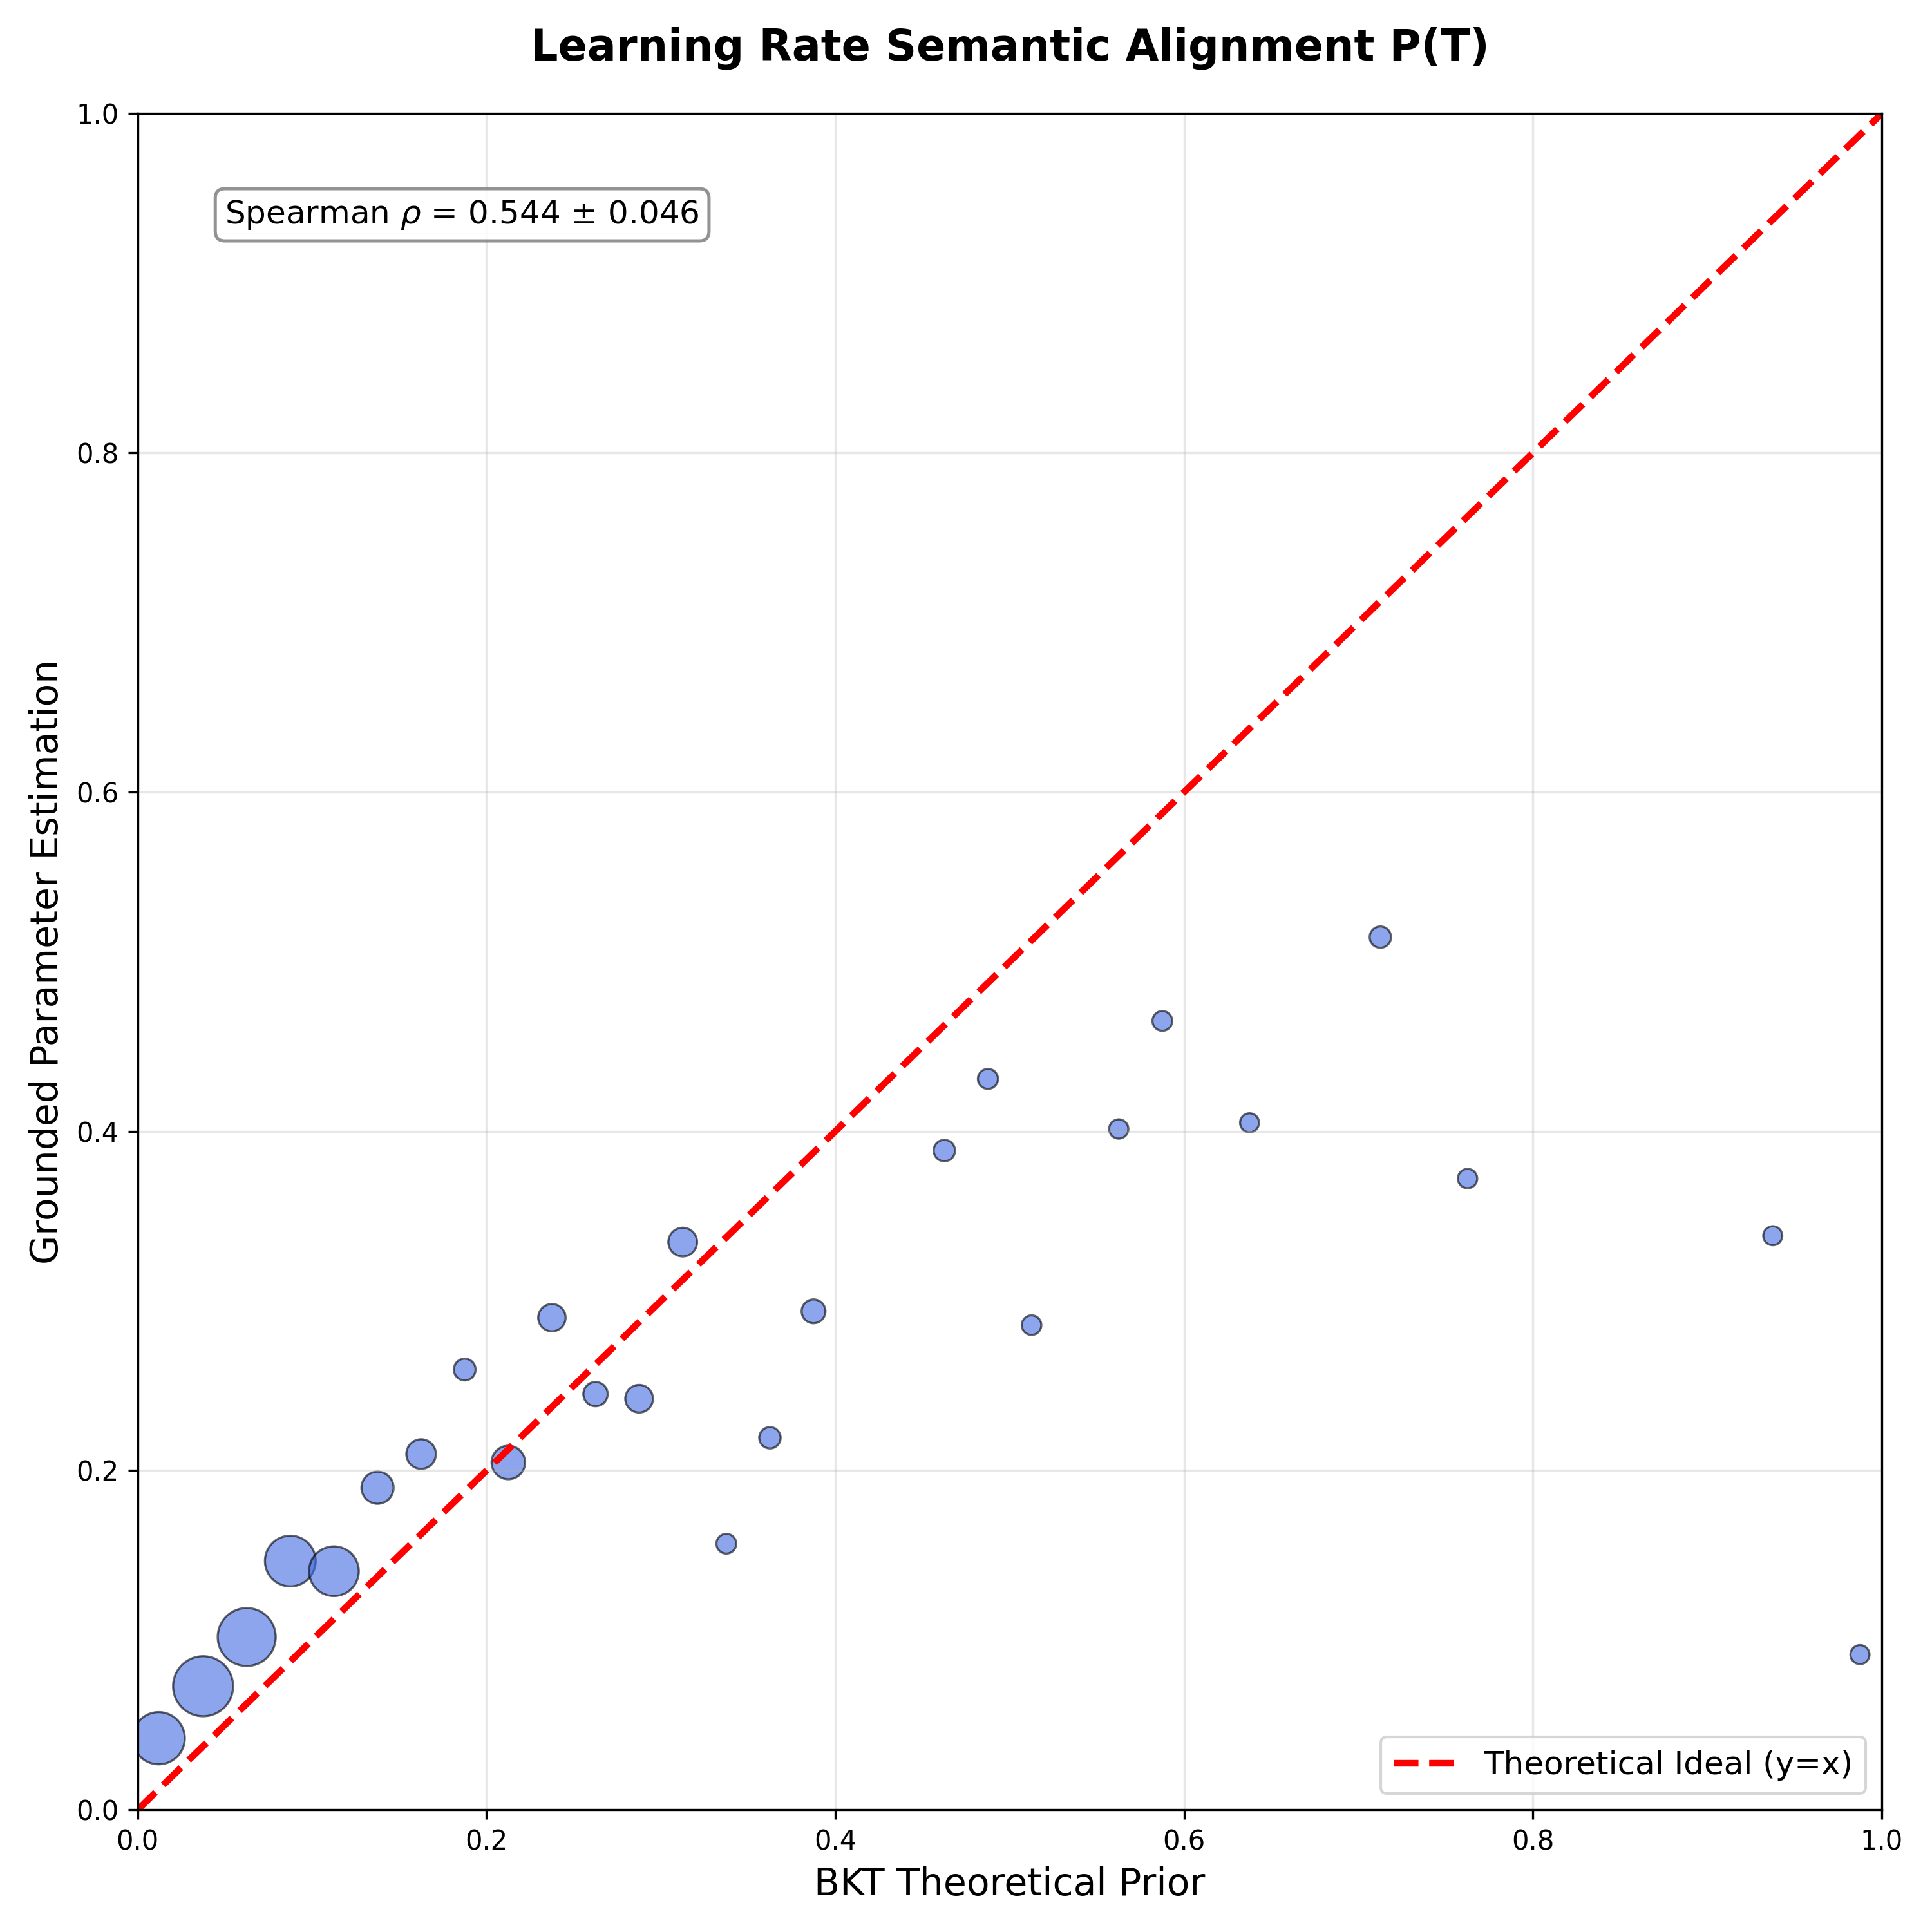
\includegraphics[width=0.68\textwidth]{img/h12_recovery_t_grounded_893468.png}
\caption{\protect\hl{Semantic} %MDPI: Please confirm whether the bubble needs an explanation. 
 alignment for learn rate $P(\text{T})$. Plot demonstrating moderate monotonic relationship preservation (Spearman $\rho = 0.544$, MAE = $0.092$) between BKT theoretical priors and grounded parameters. The~clustering around the diagonal across the full $P_{\text{T}}$ range indicates that the model preserves pedagogical understanding of practice effects through neural processing while enabling context-aware~refinement. \label{fig_semantic_alignment_t}}
\end{figure}
\unskip

\subsubsection{Functional Alignment (H2.3)} \label{sec_functional_alignment}

For the third hypothesis we compare two prediction paths: interpretable predictions $\hat{y}_{\text{ref}}$ generated by feeding enriched parameters (projected from context vectors $\mathbf{z}_t$) through BKT logic and~supervised predictions $\hat{y}_{\text{sup}}$ obtained directly from an MLP applied to $\mathbf{z}_t$. While $\hat{y}_{\text{sup}}$ uses the full representational capacity of the neural network for maximum predictive accuracy, $\hat{y}_{\text{ref}}$ constrains predictions through pedagogically interpretable BKT parameters, enabling causal explanations at the cost of some predictive power. We assess the \textit{confidence} with which the interpretable reference path can functionally replace the supervised~path.

In \Cref{fig_h13_confidence_heatmap}, we observe heterogeneous confidence patterns across AS2009 interactions. {For the generation of this heatmap, balanced weight values ($w_1 = 0.4, w_2 = 0.3, w_3 = 0.3$) were used to assign equal importance to all criteria while slightly prioritising numerical calibration.} Overall, 89.2\% of student--skill pairs achieve medium or high confidence, while only 10.8\% exhibit low confidence. This indicates that interpretable predictions provide actionable diagnostic value with quantified uncertainty, enabling educators to leverage theory-grounded explanations while {recognising} situations requiring additional~validation.

\begin{figure}[H]
%\centering
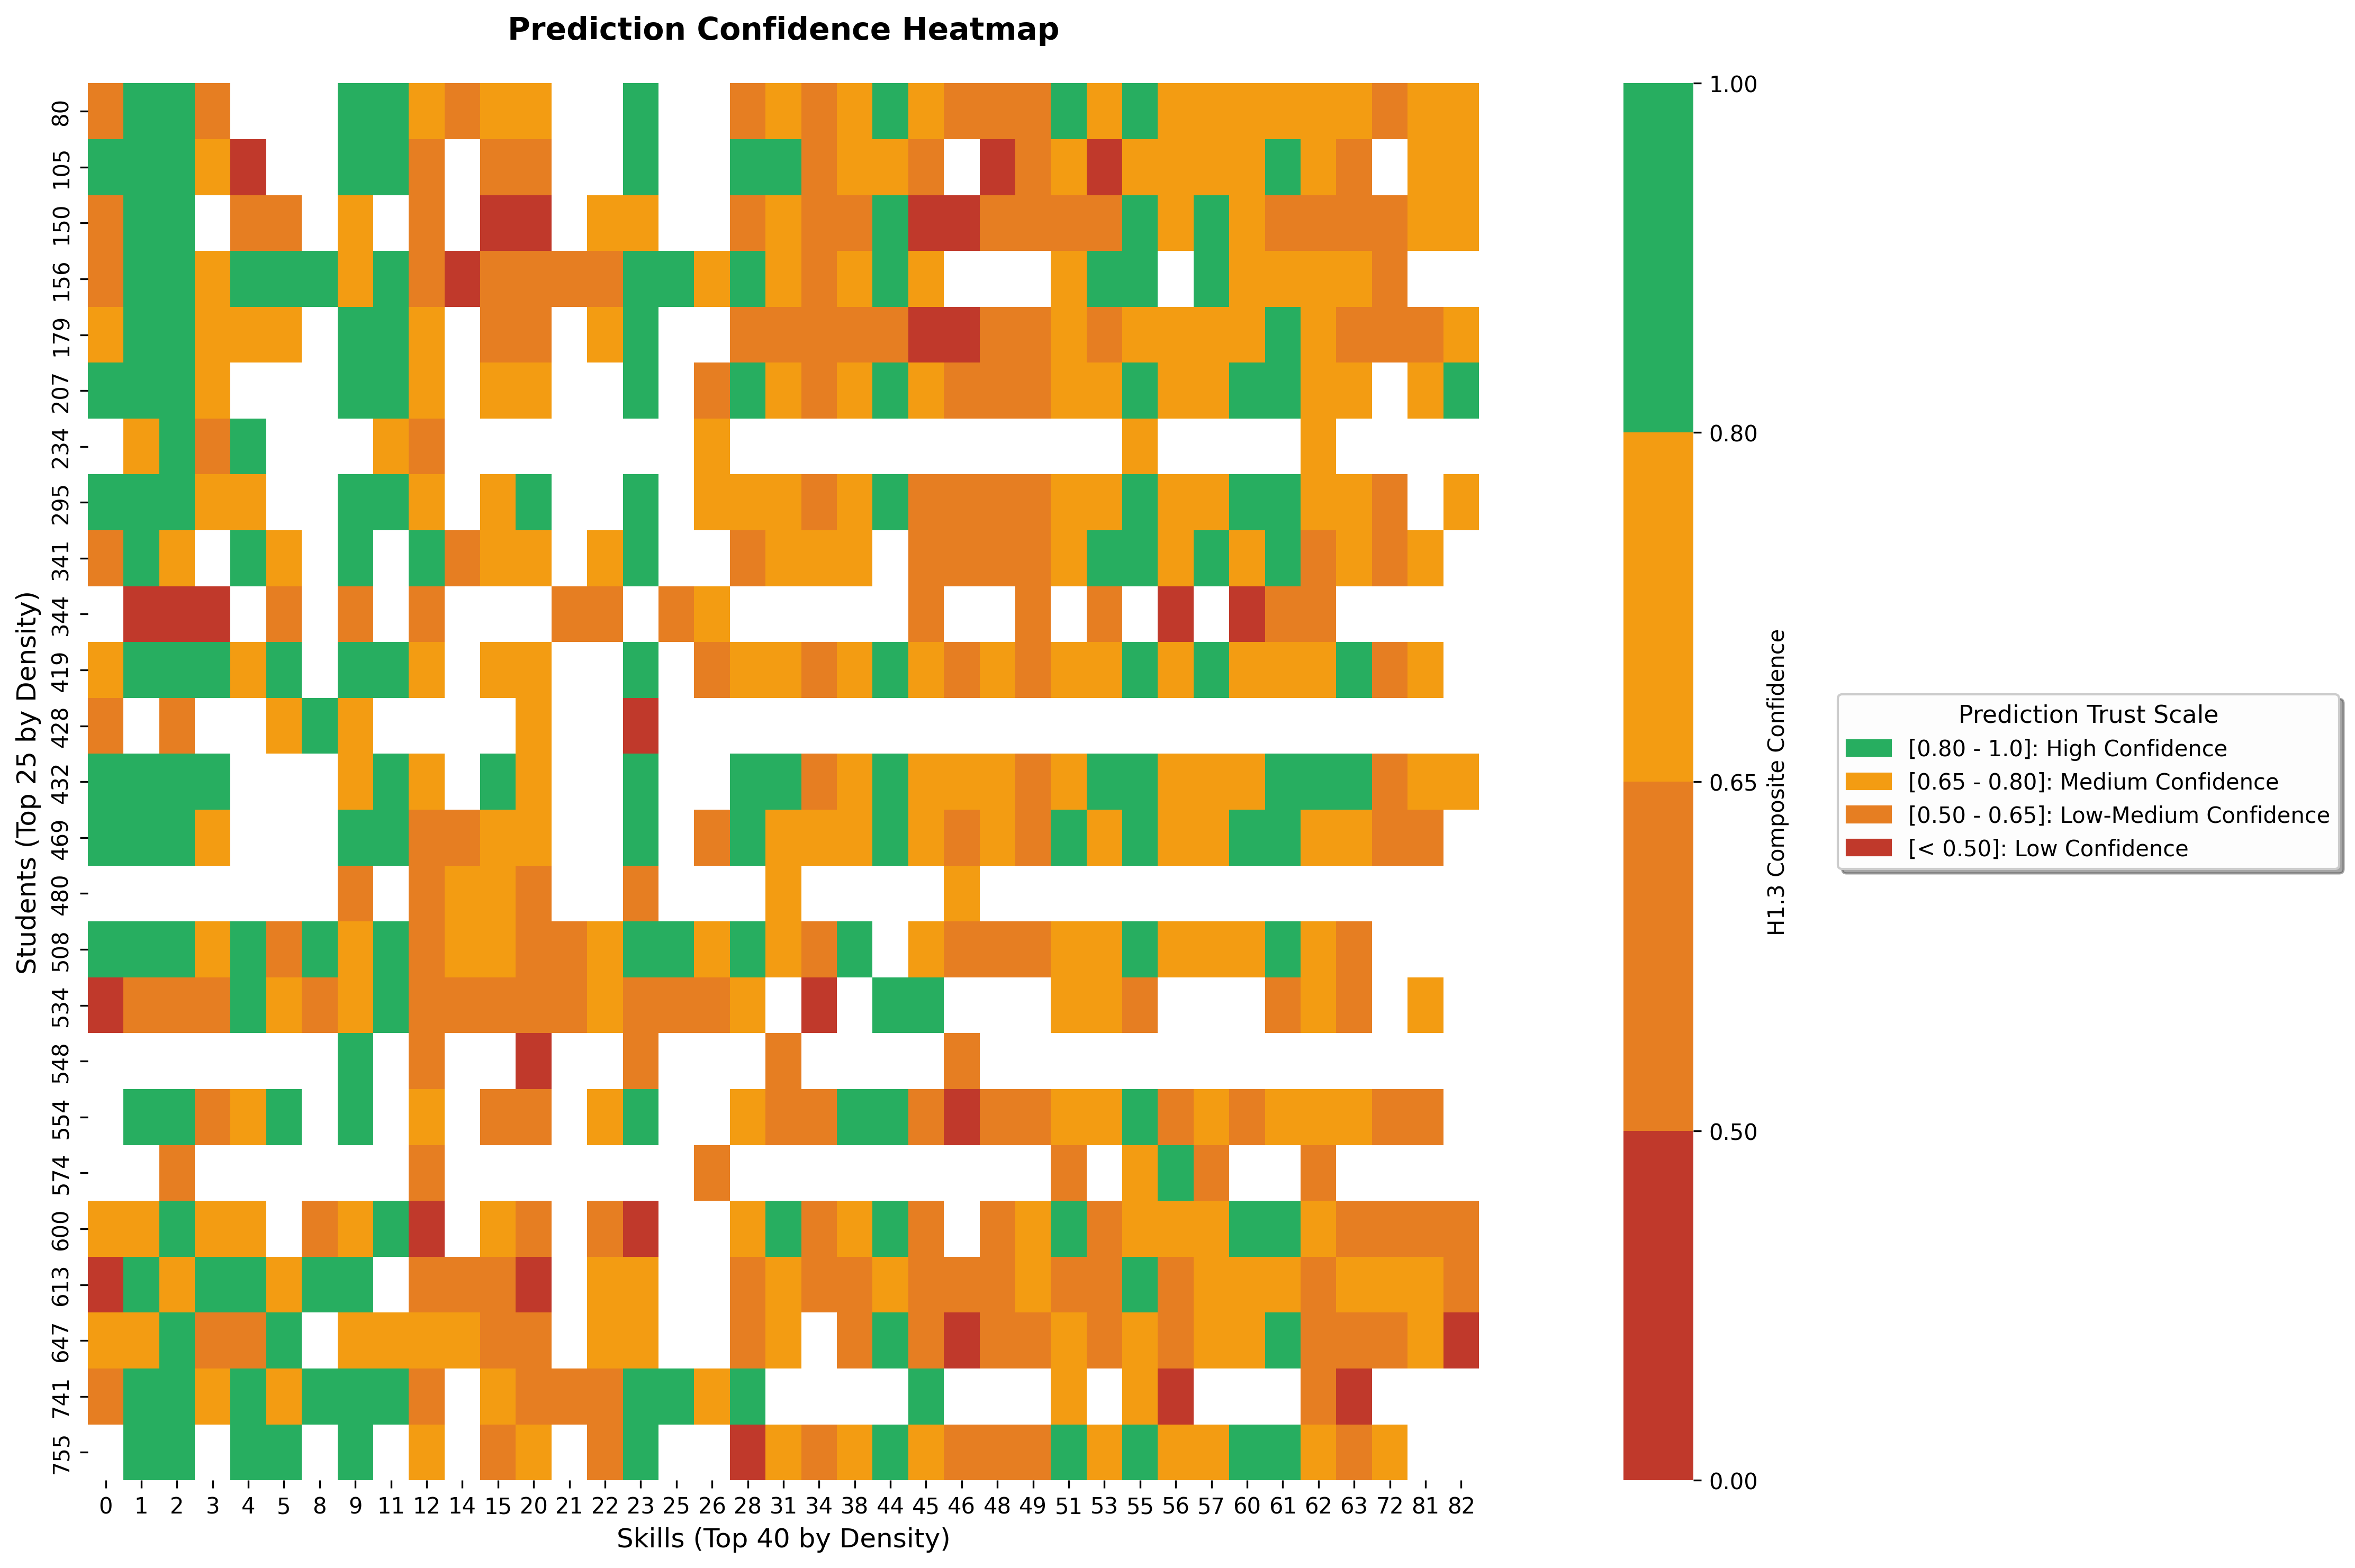
\includegraphics[width=0.85\textwidth]{img/h13_skill_confidence_heatmap_893468.png}
\caption{\protect\hl{Student} %MDPI: Please change the hyphen (-) between numbers into an en dash (−, “U+2013”), e.g., “2019-2022” should be “2019–2022” and “0-9” should be “0–9”.
  skill confidence heatmap. Green cells indicate high confidence ($\geq$0.8) in the interpretable predictions. Yellow shows medium confidence and red indicates low~confidence. \label{fig_h13_confidence_heatmap}}
\end{figure}
\unskip

\subsection{\texorpdfstring{\protect\highlighting{Context-Aware Personalisation (RQ3)}}{Context-Aware Personalisation (RQ3)}} \label{sec_gran_results}


To validate RQ3, we show how gTransformer differentiates students based on their longitudinal learning context (i.e., their sequence of interactions) rather than just response patterns. This capability enables context-aware personalisation beyond what population-based models such as BKT can provide. Classical BKT is fundamentally Markovian: given the same response sequence, it produces identical predictions regardless of the student's learning history. {The gTransformer model, by~contrast, uses its high capacity to capture temporal learning dynamics (the individualized parameters extracted from interaction history) to differentiate students even when their observable responses are identical. By~synthesising this history into a latent context vector and projecting it onto student-specific parameters ($p_{\text{L}_0}$ and $p_{\text{T}}$), the~model identifies unique learning signatures that Markovian transitions fundamentally cannot represent. This allows gTransformer to differentiate students even when their immediate observable responses are identical.}

\textls[-15]{In order to demonstrate this capability, we perform a cluster analysis on the AS2009 dataset based on the historical parameters $p_{\text{L}_0}$ and $p_{\text{T}}$ and then select representative students from each cluster to show how gTransformer can provide customized~recommendations.}  

Students are {categorised} into four learning situations based on their historical learning parameters. \Cref{fig:student_clusters_as2009} illustrates the distribution of students across the four quadrants:

\begin{itemize}
    \item Low Initial Mastery/Low Learn Rate: Observations for students in this quadrant suggest limited foundational mastery with slow skill acquisition. 
    \item Low Initial Mastery/High Learn Rate: Despite initial knowledge gaps, rapid progress indicates responsiveness to instruction. 
    \item High Initial Mastery/Low Learn Rate: Strong foundational mastery but minimal progress may signal disengagement or instructional mismatch. 
    \item High Initial Mastery/High Learn Rate: Consistent mastery and rapid skill development suggest readiness for advanced material.
\end{itemize}
\vspace{-9pt}

\begin{figure}[H]
    %\centering
    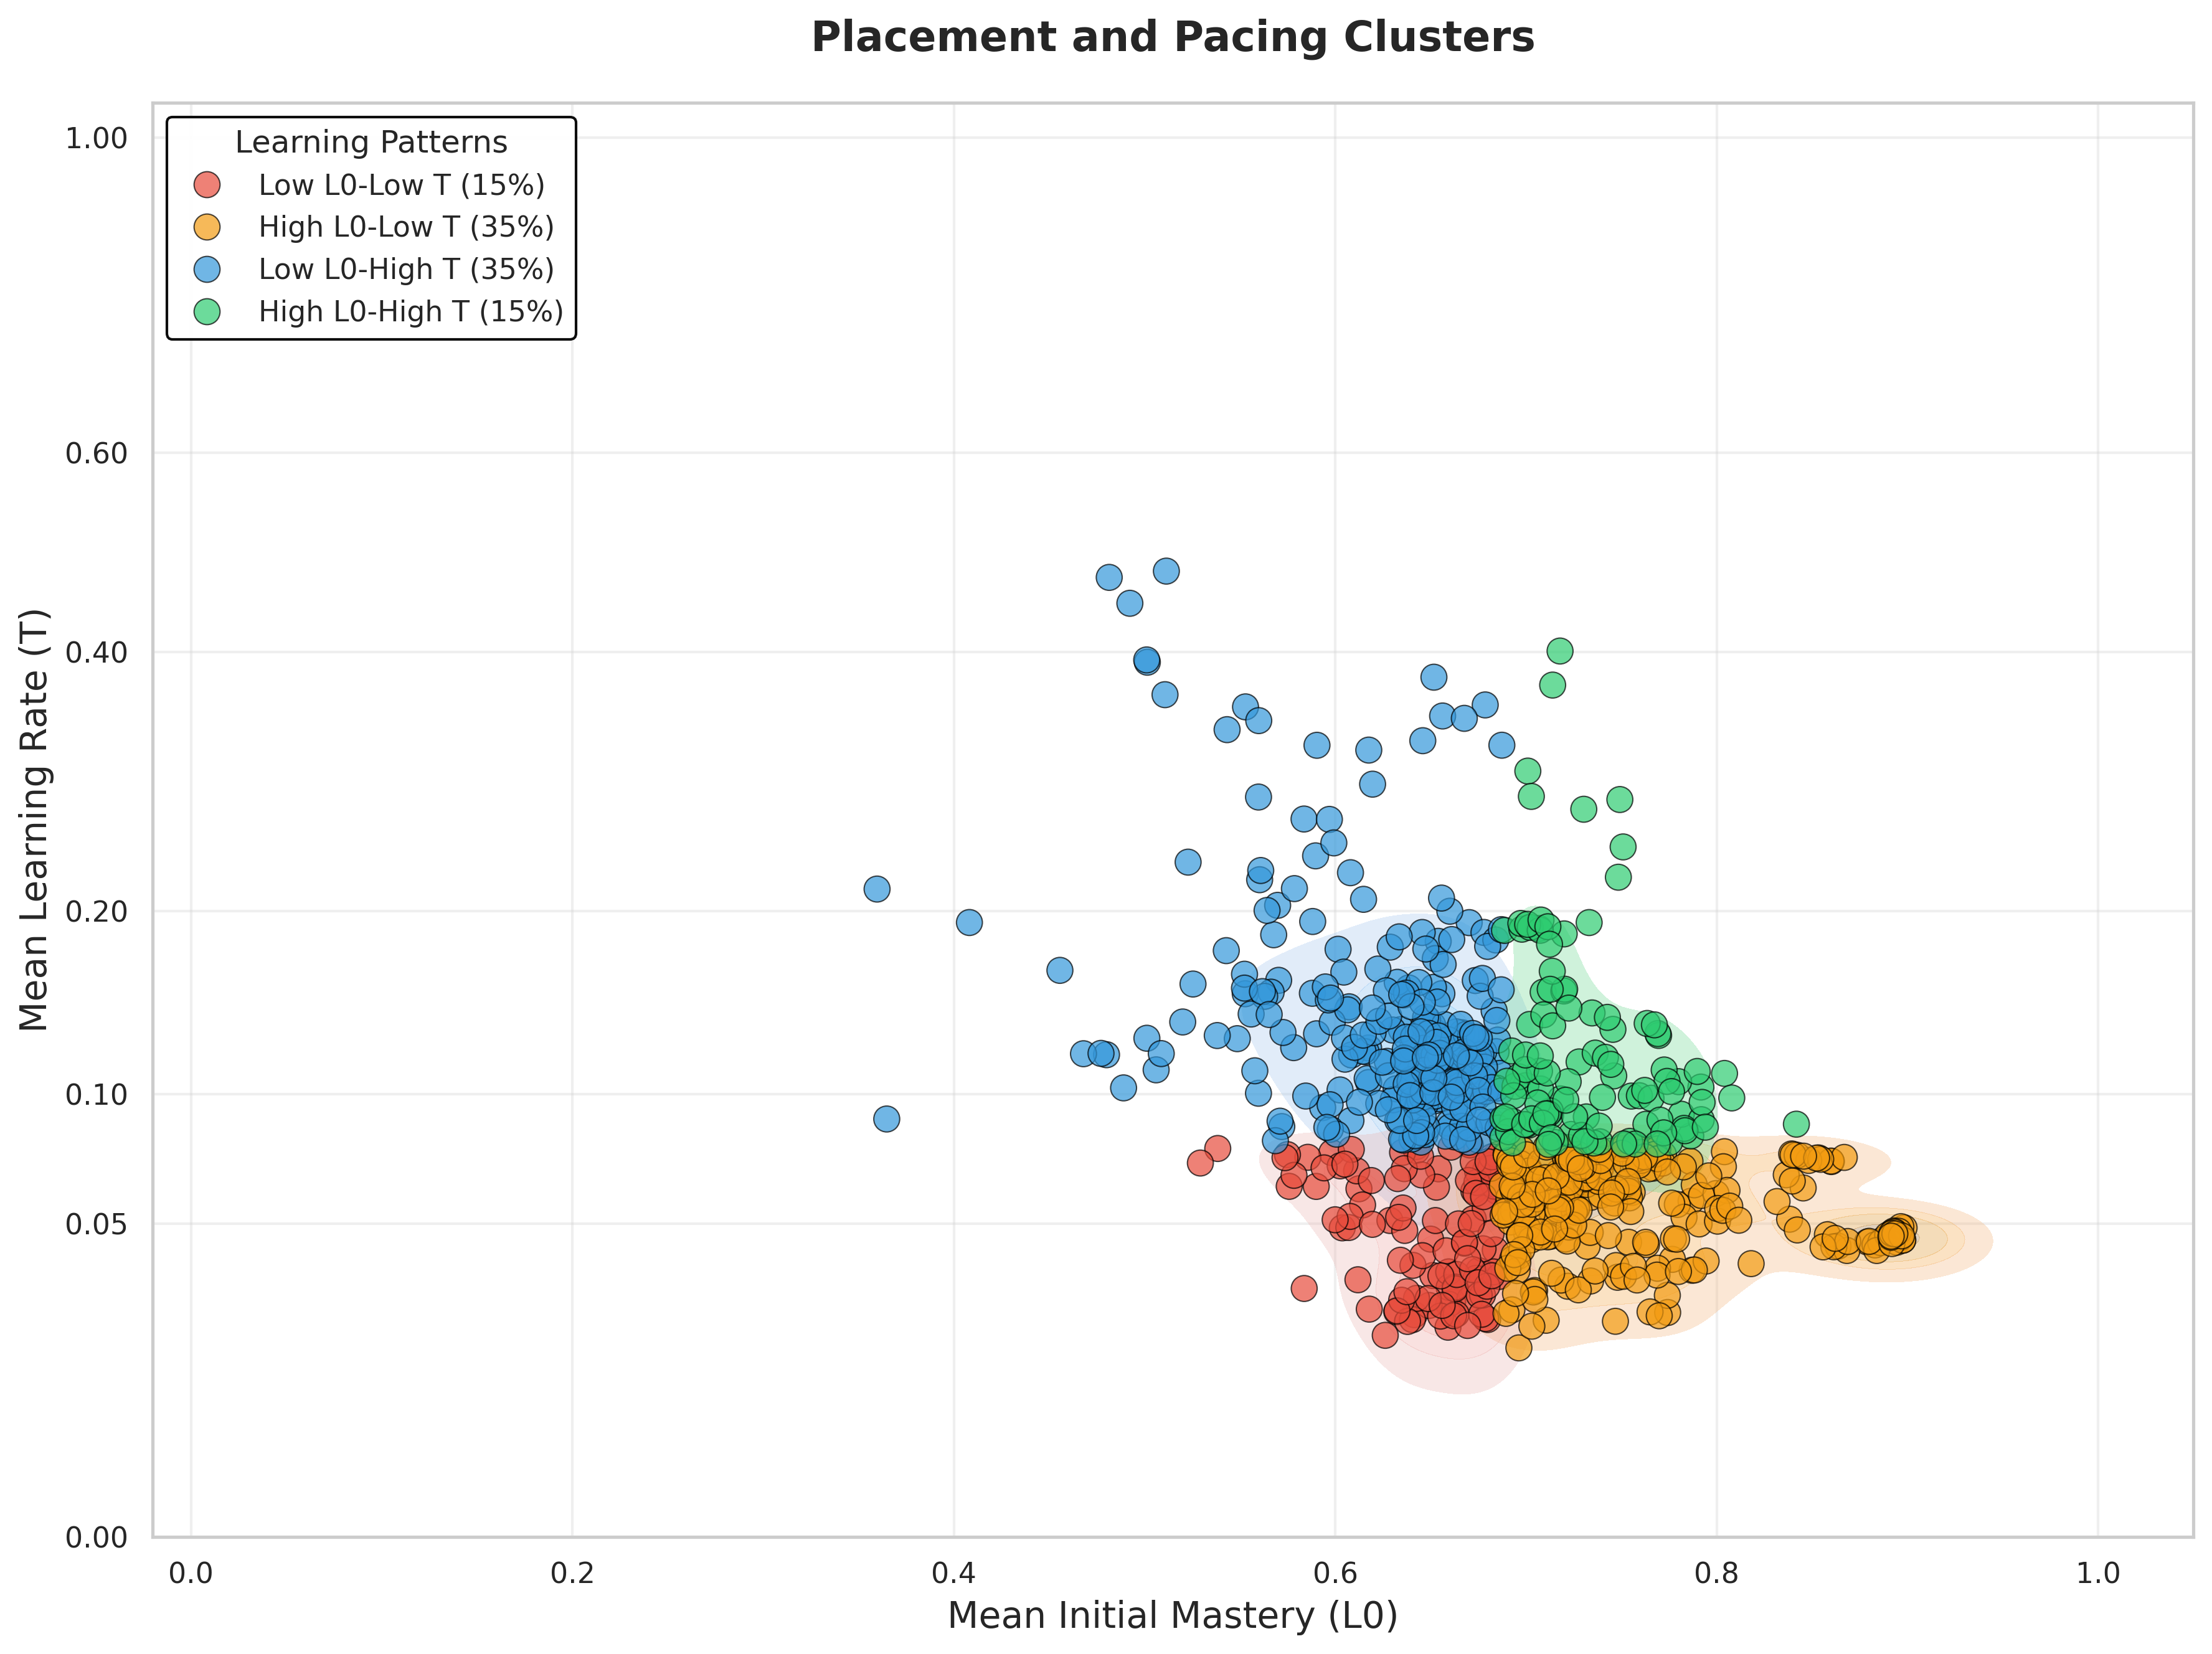
\includegraphics[width=0.8\textwidth]{img/cluster_placement_pacing_contextual_893468.png}
    \caption{Clustering of students into four learning situations based on their historical parameters (computed as averages across all previous interactions).}
    \label{fig:student_clusters_as2009}
\end{figure}


In order to demonstrate gTransformer's ability to capture historical learning context and overcome the Markovian limitations characteristic of traditional approaches, we show a comparative analysis of mastery trajectories for students with identical response~sequences. 

We select representative skills with meaningful sequence lengths (5--30 interactions) and identify students from at least two different learning quadrants who provide the same responses to the same questions in the same order. These trajectories are illustrated in the 4 $\times$ 3 mosaic shown in \cref{fig:skill_quadrant_mosaic}, where each subplot displays different predictions for students from different quadrants despite their identical performance within each skill. The~dotted {grey} BKT lines overlap perfectly, reflecting the Markovian assumption: BKT produces identical probability estimates for all students who provide the same sequence of responses, regardless of their broader learning history. In~contrast, the~solid {coloured} gTransformer lines diverge based on the whole learning trajectory, demonstrating that the model attends to historical learning context, i.e.,~to the full trajectory of previous interactions across all skills, to~differentiate students even when their current skill-specific responses are identical. This confirms that gTransformer captures non-Markovian {personalisation} patterns that classical models fundamentally cannot~represent.

\begin{figure}[H]
%\centering
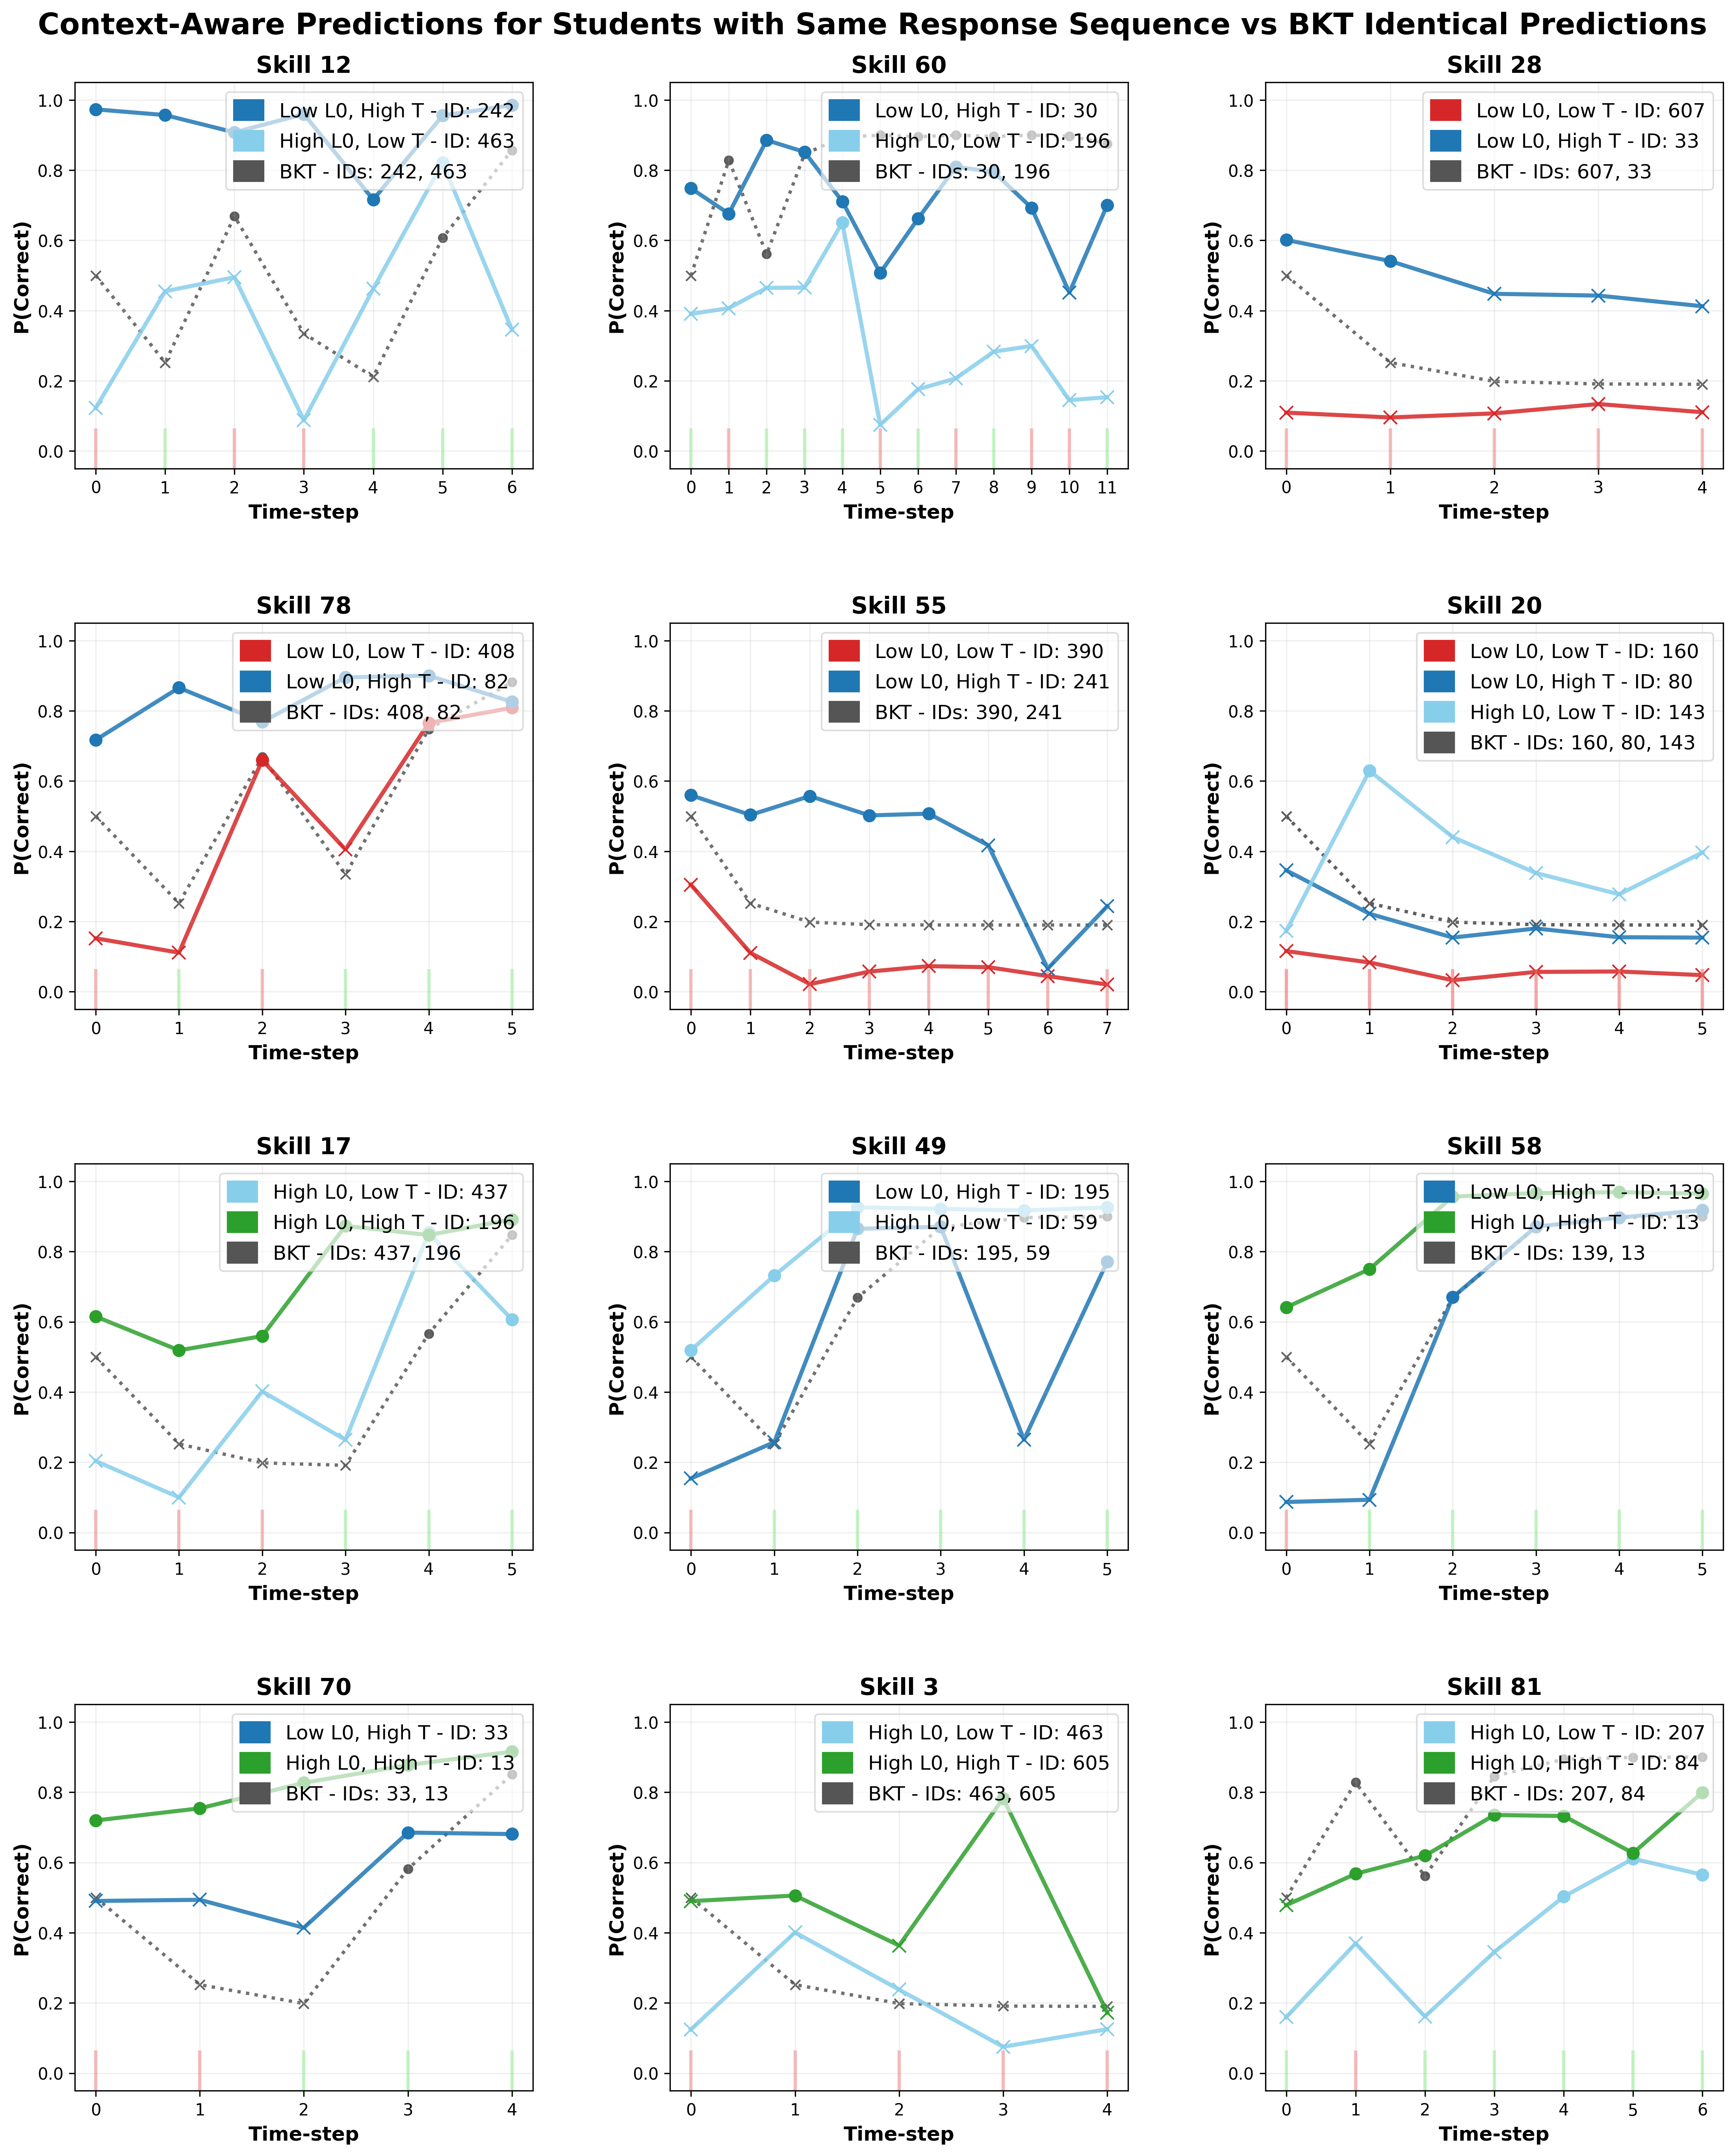
\includegraphics[width=1.0\textwidth]{img/h3_skill_quadrant_comparison_mosaic_893468.png}
\caption{\protect\hl{Context-aware} %MDPI: Please confirm whether the overlapping content in this figure affects scientific understanding and if it does, please revise it.
%MDPI: Please confirm whether the red and green vertical lines need explanation.
  prediction mosaic showing non-Markovian personalisation. Each panel displays students with identical response sequences (same ground truth bars) but different learning profiles. BKT predictions (dotted grey) overlap due to Markovian constraints, while gTransformer predictions (solid coloured) diverge based on historical parameters ($p_{\text{L}_0}, p_{\text{T}}$). Circles represent predictions of correctness, while crosses indicate predicted failures. This demonstrates that gTransformer differentiates students not by what they answered, but~by how they learned along their whole learning~trajectory.}
\label{fig:skill_quadrant_mosaic}
\end{figure}

\textls[-15]{These findings validate our hypothesis for RQ3, showing how the historical learning context captured by a Transformer-based model can enhance student-centred~personalisation.}

\subsection{Practical and Social~Implications} \label{sec_practical_social}

{By providing differentiated diagnostics based on longitudinal interaction histories, the~model acknowledges that students are dynamic learners with unique contexts rather than static entities defined by fixed traits, thereby enabling more personalised instructional interventions. For~instance, high-momentum learners can be identified for accelerated pacing to maintain engagement, while students whose profiles indicate a need for foundational remediation can receive targeted scaffolding before significant learning gaps emerge.}

\textls[-15]{In general, the~balance between accuracy and interpretability provided by our gTransformer model is crucial for promoting transparency and trust. This allows educators to clearly understand the pedagogical rationale behind the model's estimations, even for students with similar response patterns. Thus, our approach offers a practical path toward building AI tools that are not only accurate but also student-centred and pedagogically~justifiable.}

\section{Limitations and Future~Research} \label{sec_limitations_future}

{The representational grounding methodology explored in this work is fundamentally domain-independent, which suggests that the resulting pedagogical insights and the accuracy--interpretability trade-off could be generalised to diverse educational contexts.} {Nonetheless, extending the empirical validation of gTransformer beyond the benchmark datasets utilised in this study to a wider range of domains and subjects represents a valuable research direction to further demonstrate its versatility.}

{In this initial study, the~grounding process was restricted to the two primary knowledge parameters: initial mastery $P(\text{L}_0)$ and learn rate $P(\text{T})$.} {Future research could address the impact of incorporating student-specific \textit{Guess} and \textit{Slip} values to further refine the granularity of context-aware individualisation.}

{While gTransformer was validated using BKT as the primary reference model, the~underlying representational grounding approach is inherently extensible. Within~the educational domain, future research could investigate the integration of alternative theoretical frameworks, such as Additive Factor Models or Performance Factor Analysis, allowing for the use of diverse pedagogical parameters while leveraging the Transformer architecture's awareness of the historical learning context. Furthermore, the~applicability of the gTransformer approach extends beyond Knowledge Tracing. The~representational grounding framework can be adapted to any scientific field where established theoretical models coexist with high-volume empirical data. By~anchoring latent representations to domain-specific concepts, this methodology offers a {generalisable} path toward bridging deep learning expressiveness with rigorous scientific grounding. Evaluating how different theoretical assumptions influence both the accuracy--interpretability trade-off and the context-awareness of domain-specific predictions across diverse disciplines remains an open and promising avenue for future research.}

\section{Conclusions} \label{sec_conclusions}

This work introduces gTransformer, a~Transformer-based model that bridges the gap between deep learning performance and intrinsic interpretability through representational grounding. By~anchoring latent representations to semantically meaningful constructs, we demonstrate that competitive predictive accuracy can coexist with theoretical~alignment.

Our results validate the approach across three dimensions. First, quantifying the accuracy--interpretability trade-off, we showed that interpretable gTransformer predictions consistently surpass classical BKT with a low interpretability cost relative to black-box architectures (RQ1). Second, we confirmed that gTransformer {internalises} BKT constructs as its primary {organising} principle, achieving high structural selectivity and semantic alignment with theoretical priors (RQ2). Finally, we demonstrated that gTransformer enables context-aware {personalisation} by capturing longitudinal learning patterns that Markovian models inherently overlook, allowing for differentiated diagnostics for students with similar response patterns but different interaction histories (RQ3).

Ultimately, gTransformer provides a practical approach for transforming opaque deep learning predictors into actionable interpretable tools. {By grounding high-capacity models in established domain theory, this approach offers a path toward highly accurate, pedagogically justifiable, and~context-aware personalisation.}

%%%%%%%%%%%%%%%%%%%%%%%%%%%%%%%%%%%%%%%%%%
\vspace{6pt} 

%%%%%%%%%%%%%%%%%%%%%%%%%%%%%%%%%%%%%%%%%%
%% optional
%\supplementary{The following supporting information can be downloaded at:  \linksupplementary{s1}, Figure S1: title; Table S1: title; Video S1: title.}

% Only for journal Methods and Protocols:
% If you wish to submit a video article, please do so with any other supplementary material.
% \supplementary{The following supporting information can be downloaded at: \linksupplementary{s1}, Figure S1: title; Table S1: title; Video S1: title. A supporting video article is available at doi: link.}

% Only used for preprtints:
% \supplementary{The following supporting information can be downloaded at the website of this paper posted on \href{https://www.preprints.org/}{Preprints.org}.}

% Only for journal Hardware:
% If you wish to submit a video article, please do so with any other supplementary material.
% \supplementary{The following supporting information can be downloaded at: \linksupplementary{s1}, Figure S1: title; Table S1: title; Video S1: title.\vspace{6pt}\\
%\begin{tabularx}{\textwidth}{lll}
%\toprule
%\textbf{Name} & \textbf{Type} & \textbf{Description} \\
%\midrule
%S1 & Python script (.py) & Script of python source code used in XX \\
%S2 & Text (.txt) & Script of modelling code used to make Figure X \\
%S3 & Text (.txt) & Raw data from experiment X \\
%S4 & Video (.mp4) & Video demonstrating the hardware in use \\
%... & ... & ... \\
%\bottomrule
%\end{tabularx}
%}

%%%%%%%%%%%%%%%%%%%%%%%%%%%%%%%%%%%%%%%%%%
\authorcontributions{Conceptualisation, C.L.; methodology, C.L. and O.C.S.; software, C.L.; validation, C.L. and O.C.S.; formal analysis, C.L.; investigation, C.L.; resources, C.L. and O.C.S.; data curation, C.L.; writing---original draft preparation, C.L.; writing---review and editing, C.L. and O.C.S.; visualisation, C.L.; supervision, O.C.S. All authors have read and agreed to the published version of the manuscript.}

\funding{This research received no external~funding.}


\institutionalreview{\hl{please add}}
%MDPI: In this section, you should add the Institutional Review Board Statement and approval number, if relevant to your study. You might choose to exclude this statement if the study did not require ethical approval. Please note that the Editorial Office might ask you for further information. Please add “The study was conducted in accordance with the Declaration of Helsinki, and approved by the Institutional Review Board (or Ethics Committee) of NAME OF INSTITUTE (protocol code XXX and date of approval).” for studies involving humans. OR “The animal study protocol was approved by the Institutional Review Board (or Ethics Committee) of NAME OF INSTITUTE (protocol code XXX and date of approval).” for studies involving animals. OR “Ethical review and approval were waived for this study due to REASON (please provide a detailed justification).” OR “Not applicable” for studies not involving humans or animals.

\informedconsent{\hl{please add}}
%MDPI: Any research article describing a study involving humans should contain this statement. Please add ``Informed consent was obtained from all subjects involved in the study.'' OR ``Patient consent was waived due to REASON (please provide a detailed justification).'' OR ``Not applicable'' for studies not involving humans. You might also choose to exclude this statement if the study did not involve humans.

%Written informed consent for publication must be obtained from participating patients who can be identified (including by the patients themselves). Please state ``Written informed consent has been obtained from the patient(s) to publish this paper'' if applicable.


\dataavailability{The datasets used in this paper can be downloaded through the links provided \hl{in} %MDPI: Please provide the date you accessed the URL in the following format: “URL (accessed on Day Month Year)”.
 \url{https://pykt-toolkit.readthedocs.io/en/latest/datasets.html}.}

\conflictsofinterest{The authors declare no conflicts of~interest.} 

%%%%%%%%%%%%%%%%%%%%%%%%%%%%%%%%%%%%%%%%%%
\begin{adjustwidth}{-\extralength}{0cm}
%\printendnotes[custom] % Un-comment to print a list of endnotes

\reftitle{References}

% Please provide either the correct journal abbreviation (e.g. according to the "List of Title Word Abbreviations" http://www.issn.org/services/online-services/access-to-the-ltwa/) or the full name of the journal.
% Citations and References in Supplementary files are permitted provided that they also appear in the reference list here. 

%=====================================
% References, variant A: external bibliography
%=====================================
\begin{thebibliography}{999}

\bibitem[Corbett and Anderson(1994)]{corbett1994knowledge}
Corbett, A.T.; Anderson, J.R.
\newblock Knowledge tracing: Modeling the acquisition of procedural knowledge.
\newblock {\em User Model. User-Adapt. Interact.} {\bf 1994}, {\em
  4},~253--278.

\bibitem[Romero and Ventura(2020)]{Romero2020}
Romero, C.; Ventura, S.
\newblock Educational data mining and learning analytics: An updated survey.
\newblock {\em Wiley Interdiscip. Rev. Data Min. Knowl. Discov.} {\bf 2020}, {\em 10}, \hl{e1355}%MDPI: we removed extra content, please confirm all.
.
  {\url{https://doi.org/10.1002/widm.1355}}.

\bibitem[Abdelrahman et~al.(2023)Abdelrahman, Wang, and
  Nunes]{abdelrahman2023knowledge}
Abdelrahman, G.; Wang, Q.; Nunes, B.
\newblock Knowledge tracing: A survey.
\newblock {\em ACM Comput. Surv.} {\bf 2023}, {\em 55},~1--37.

\bibitem[Ines et~al.(2024)Ines, Ani, and Angelina]{twenty_five_years_of_bkt}
Ines, {\v{S}ari\'c-Grgi\'c}.; Ani, G.; Angelina, G.
\newblock Twenty-Five Years of Bayesian knowledge tracing: a systematic review.
\newblock {\em User Model. User-Adapt. Interact.} {\bf 2024}, {\em
  34},~1127–1173.
\newblock  {\url{https://doi.org/10.1007/s11257-023-09389-4}}.

\bibitem[Vaswani et~al.(2017)Vaswani, Shazeer, Parmar, Uszkoreit, Jones, Gomez,
  Kaiser, and Polosukhin]{vaswani2017attention}
\added[id=revproof]{Vaswani, A.; Shazeer, N.; Parmar, N.; Uszkoreit, J.; Jones, L.; Gomez, A.N.; Kaiser, L.; Polosukhin, I. Attention is all you need. Advances in Neural Information Processing Systems, bf 30, 2017.}
%AuthorsAnswer: Updated this citation to the published conference version instead of the arXiv preprint. See biblio.bib file for reference details.

\bibitem[Bai et~al.(2024)Bai, Zhao, Wei, Cai, and He]{bai2024survey}
Bai, Y.; Zhao, J.; Wei, T.; Cai, Q.; He, L.
\newblock A survey of explainable knowledge tracing.
\newblock {\em Appl. Intell.} {\bf 2024}, {\em 54},~6483--6514.

\bibitem[Rudin(2019)]{rudin2019stop}
Rudin, C.
\newblock Stop explaining black box machine learning models for high stakes
  decisions and use interpretable models instead.
\newblock {\em Nat. Mach. Intell.} {\bf 2019}, {\em 1},~206--215.

\bibitem[Von~Rueden et~al.(2021)Von~Rueden, Mayer, Beckh, Georgiev,
  Giesselbach, Heese, Kirsch, Pfrommer, Pick, Ramamurthy, Walczak, Garcke,
  Bauckhage, and Schuecker]{vonrueden2021informed}
Von~Rueden, L.; Mayer, S.; Beckh, K.; Georgiev, B.; Giesselbach, S.; Heese, R.;
  Kirsch, B.; Pfrommer, J.; Pick, A.; Ramamurthy, R.;  et~al.
\newblock Informed Machine Learning---A Taxonomy and Survey of Integrating
  Knowledge into Learning Systems.
\newblock {\em IEEE Trans. Knowl. Data Eng.} {\bf 2021}, \textit{35},
  614--633.

\bibitem[Holmes et~al.(2022)Holmes, Porayska-Pomsta, Holstein, Sutherland,
  Baker, Shum, Santos, Rodrigo, Cukurova, Bittencourt, and
  Koedinger]{Holmes2022504}
Holmes, W.; Porayska-Pomsta, K.; Holstein, K.; Sutherland, E.; Baker, T.; Shum,
  S.B.; Santos, O.C.; Rodrigo, M.T.; Cukurova, M.; Bittencourt, I.I.;  et~al.
\newblock Ethics of AI in Education: Towards a Community-Wide Framework.
\newblock {\em Int. J. Artif. Intell. Educ.}
  {\bf 2022}, {\em 32},~504–526.
\newblock 
  {\url{https://doi.org/10.1007/s40593-021-00239-1}}.

\bibitem[Cen et~al.(2008)Cen, Koedinger, and Junker]{cen2008comparing}
Cen, H.; Koedinger, K.; Junker, B.
\newblock Comparing two IRT models for conjunctive skills.
\newblock In \textit{Proceedings of the International Conference on Intelligent
  Tutoring Systems}; Springer: \hl{Berlin/Heidelberg, Germany}, %We added the location of publisher. Please confirm. Same below.
 2008; pp. 796--798.

\bibitem[Pavlik et~al.(2009)Pavlik, Cen, and Koedinger]{pavlik2009performance}
Pavlik, P.I.; Cen, H.; Koedinger, K.R.
\newblock Performance factors analysis - A new alternative to knowledge
  tracing.
\newblock {\em Front. Artif. Intell. Appl.} {\bf
  2009}, {\em 200},~531–538.
\newblock  {\url{https://doi.org/10.3233/978-1-60750-028-5-531}}.

\bibitem[Vie and Kashima(2019)]{vie2019knowledge}
Vie, J.J.; Kashima, H.
\newblock Knowledge tracing machines: Factorization machines for knowledge
  tracing.
\newblock In \textit{Proceedings of the AAAI Conference on
  Artificial Intelligence}; \hl{AAAI Press: Washington, DC, USA}%MDPI: We added the name of the publisher and their location. Please confirm. Same below.
, 2019; Volume~33, pp. 750--757.

\bibitem[Embretson and Reise(2013)]{embretson2013item}
Embretson, S.E.; Reise, S.P.
\newblock {\em Item Response Theory for Psychologists}; Psychology Press: \hl{Hove, UK},
  2013.


\bibitem[Piech et~al.(2015)Piech, Bassen, Huang, Ganguli, Sahami, Guibas, and Sohl-Dickstein]{piech2015deep}
\added[id=revproof]{%
Piech, C.; Bassen, J.; Huang, J.; Ganguli, S.; Sahami, M.; Guibas, L.J.; Sohl-Dickstein, J.
\newblock Deep knowledge tracing.
\newblock \em Advances in Neural Information Processing Systems, \bf 28, 2015.%
}
%AuthorsAnswer: Updated this citation from the arXiv preprint to the formally published journal article. See biblio.bib file for reference details.

\bibitem[Pandey and Karypis(2019)]{Pandey2019384}
Pandey, S.; Karypis, G.
\newblock A self-attentive model for knowledge tracing.
\newblock In \textit{Proceedings of the 12th International
  Conference on Educational Data Mining (EDM 2019)}; International Educational
  Data Mining Society: \hl{Montreal, QC, Canada},  2019; pp. 384--389.
\newblock 

\bibitem[Ghosh et~al.(2020)Ghosh, Heffernan, and Lan]{ghosh2020context}
Ghosh, A.; Heffernan, N.; Lan, A.S.
\newblock Context-aware attentive knowledge tracing.
\newblock In Proceedings of the 26th ACM SIGKDD International Conference on
  Knowledge Discovery \& Data Mining, \hl{Virtual, 6--10 July} %MDPI: We added the location and date of the conference. Please confirm.
 2020; pp. 2330--2339.

\bibitem[Yeung(2019)]{yeung2019deep}
Yeung, C.K.
\newblock Deep-IRT: Make deep learning based knowledge tracing explainable
  using item response theory.
\newblock In \textit{Proceedings of the 12th International
  Conference on Educational Data Mining (EDM 2019)}; International Educational
  Data Mining Society: \hl{Worcester, MA, USA},  2019; pp. 683--686.


\bibitem[Su et~al.(2021)Su, Cheng, Luo, Wu, Zhang, Liu, and Wang]{su2021time}
Su, Y.; Cheng, Z.; Luo, P.; Wu, J.; Zhang, L.; Liu, Q.; Wang, S.
\newblock Time-and-concept enhanced deep multidimensional item response theory
  for interpretable knowledge tracing.
\newblock {\em Knowl.-Based Syst.} {\bf 2021}, {\em 218},~106819.

\bibitem[Chen et~al.(2023)Chen, Liu, Huang, Liu, and Luo]{chen2023improving}
Chen, J.; Liu, Z.; Huang, S.; Liu, Q.; Luo, W.
\newblock Improving interpretability of deep sequential knowledge tracing
  models with question-centric cognitive representations.
\newblock In \textit{Proceedings of the AAAI Conference on
  Artificial Intelligence}; \hl{AAAI Press: Washington, DC, USA},  2023; Volume~37, pp. 14196--14204.

\bibitem[Arnau-González et~al.(2025)Arnau-González, Wu, Solera-Monforte,
  Arnau, and Arevalillo-Herráez]{Arnau-Gonzalez2025195}
Arnau-González, P.; Wu, Y.; Solera-Monforte, S.; Arnau, D.;
  Arevalillo-Herráez, M.
\newblock Predicting User Actions in Algebra Intelligent Tutoring Systems
  with Markov Models.
\newblock {\em Lect. Notes Comput. Sci.} {\bf 2025}, {\em 15881
  LNAI},~195–202.
\newblock {\url{https://doi.org/10.1007/978-3-031-98462-4_25}}.

\bibitem[Yudelson et~al.(2013)Yudelson, Koedinger, and
  Gordon]{yudelson2013individualized}
Yudelson, M.V.; Koedinger, K.R.; Gordon, G.J.
\newblock Individualized bayesian knowledge tracing models.
\newblock In \textit{Proceedings of the International Conference on Artificial
  Intelligence in Education}; Springer: \hl{Berlin/Heidelberg, Germany},  2013; pp. 171--180.

\bibitem[Pascanu et~al.(2013)Pascanu, Mikolov, and Bengio]{Pascanu20132347}
Pascanu, R.; Mikolov, T.; Bengio, Y.
\newblock On the difficulty of training recurrent neural networks.
\newblock In P\textit{roceedings of the 30th International
  Conference on Machine Learning (ICML 2013)}; International Machine Learning
  Society (IMLS): \hl{San Diego, CA, USA},  2013; \mbox{pp. 2347--2355}.


\bibitem[Choi et~al.(2020)Choi, Lee, Cho, Baek, Kim, Cha, Shin, Bae, and
  Heo]{choi2020towards}
Choi, Y.; Lee, Y.; Cho, J.; Baek, J.; Kim, B.; Cha, Y.; Shin, D.; Bae, C.; Heo,
  J.
\newblock Towards an appropriate query, key, and value computation for
  knowledge tracing.
\newblock In \textit{Proceedings of the Seventh ACM Conference on
  Learning@ Scale}; \hl{Association for Computing Machinery: New York, NY, USA}, 2020; pp. 341--344.

\bibitem[Bach et~al.(2015)Bach, Binder, Montavon, Klauschen, M{\"u}ller, and
  Samek]{bach2015pixel}
Bach, S.; Binder, A.; Montavon, G.; Klauschen, F.; M{\"u}ller, K.R.; Samek, W.
\newblock On pixel-wise explanations for non-linear classifier decisions by
  layer-wise relevance propagation.
\newblock {\em PloS ONE} {\bf 2015}, {\em 10},~e0130140.

\bibitem[Ribeiro et~al.(2016)Ribeiro, Singh, and Guestrin]{ribeiro2016should}
Ribeiro, M.T.; Singh, S.; Guestrin, C.
\newblock ``Why should I trust you?" Explaining the predictions of any
  classifier.
\newblock In Proceedings of the 22nd ACM SIGKDD
  International Conference on Knowledge Discovery and Data Mining, \hl{San Francisco, CA, USA, 13--17 August} 2016; pp.
  1135--1144.

\bibitem[Gan et~al.(2020)Gan, Sun, and Sun]{gan2020knowledge}
Gan, W.; Sun, Y.; Sun, Y.
\newblock Knowledge interaction enhanced knowledge tracing for learner
  performance prediction.
\newblock In \textit{Proceedings of the 2020 7th International Conference on
  Behavioural and Social Computing (BESC), \hl{Bournemouth, UK, 5--7 November 2020}}; IEEE: \hl{Piscataway, NJ, USA},  2020; pp. 1--6.

\bibitem[Zhou et~al.(2021)Zhou, Li, Cao, Zhao, Ye, and Lv]{zhou2021lana}
Zhou, Y.; Li, X.; Cao, Y.; Zhao, X.; Ye, Q.; Lv, J.
\newblock LANA: Towards Personalized Deep Knowledge Tracing Through
  Distinguishable Interactive Sequences.
\newblock In \textit{Proceedings of the 14th International
  Conference on Educational Data Mining (EDM 2021)}; International Educational
  Data Mining Society: \hl{Worcester, MA, USA},  2021; pp. 602--608.


\bibitem[Liu et~al.(2022)Liu, Yu, Li, Liang, Zhang, Shen, and
  Sun]{liu2022ability}
Liu, S.; Yu, J.; Li, Q.; Liang, R.; Zhang, Y.; Shen, X.; Sun, J.
\newblock Ability boosted knowledge tracing.
\newblock {\em Inf. Sci.} {\bf 2022}, {\em 596},~567--587.

\bibitem[Sun et~al.(2024)Sun, Wei, Feng, Yu, Li, and Zou]{sun2024progressive}
Sun, J.; Wei, M.; Feng, J.; Yu, F.; Li, Q.; Zou, R.
\newblock Progressive knowledge tracing: Modeling learning process from
  abstract to concrete.
\newblock {\em Expert Syst. Appl.} {\bf 2024}, {\em 238},~122280.

\bibitem[Zhang(2021)]{zhang2021learning}
Zhang, L.
\newblock Learning factors knowledge tracing model based on dynamic cognitive
  diagnosis.
\newblock {\em Math. Probl. Eng.} {\bf 2021}, {\em
  2021},~8777160.

\bibitem[Zhu et~al.(2020)Zhu, Yu, Zheng, Huang, Tang, and
  Fung]{zhu2020learning}
Zhu, J.; Yu, W.; Zheng, Z.; Huang, C.; Tang, Y.; Fung, G.P.C.
\newblock Learning from interpretable analysis: Attention-based knowledge
  tracing.
\newblock In \textit{Proceedings of the International Conference on Artificial
  Intelligence in Education}; Springer: \hl{Berlin/Heidelberg, Germany},  2020; pp. 364--368.

\bibitem[Lee et~al.(2024)Lee, Park, Kim, Choi, and Kim]{lee2024monacobert}
Lee, U.; Park, Y.; Kim, Y.; Choi, S.; Kim, H.
\newblock Monacobert: Monotonic attention based convbert for knowledge tracing.
\newblock In \textit{Proceedings of the International Conference on Intelligent
  Tutoring Systems}; Springer: \hl{Berlin/Heidelberg, Germany},  2024; pp. 107--123.

\bibitem[Zhang et~al.(2023)Zhang, Zhu, Zhang, Qian, Pan, and
  Zhao]{zhang2023counterfactual}
Zhang, M.; Zhu, X.; Zhang, C.; Qian, W.; Pan, F.; Zhao, H.
\newblock Counterfactual Monotonic Knowledge Tracing for Assessing Students'
  Dynamic Mastery of Knowledge Concepts.
\newblock In Proceedings of the 32nd ACM International
  Conference on Information and Knowledge Management, \hl{Birmingham, UK, 21--25 October} 2023; pp. 3236--3246.

\bibitem[Labra and Santos(2023)]{labra2023exploring}
Labra, C.; Santos, O.C.
\newblock Exploring cognitive models to augment explainability in Deep
  Knowledge Tracing.
\newblock In \textit{Proceedings of the Adjunct Proceedings of the 31st ACM Conference
  on User Modeling, Adaptation and Personalization (UMAP '23 Adjunct)}; \hl{Association for Computing Machinery: New York, NY, USA},  2023;
  pp. 220--223.
\newblock {\url{https://doi.org/10.1145/3563359.3597384}}.


\bibitem[Badrinath and Pardos(2025)]{badrinath2025optimizing}
\added[id=revproof]{%
Badrinath, A.; Pardos, Z.
\newblock Optimizing Bayesian Knowledge Tracing with Neural Network Parameter Generation.
\newblock Journal of Educational Data Mining, \bf 17 (1), 41--65, 2025.%
}
%AuthorsAnswer: Updated this citation from the arXiv preprint to the formally published journal article. See biblio.bib file for reference details.

\bibitem[Karpatne et~al.(2017)Karpatne, Atluri, Faghmous, Steinbach, Banerjee,
  Ganguly, Shekhar, Samatova, and Kumar]{karpatne2017theory}
Karpatne, A.; Atluri, G.; Faghmous, J.; Steinbach, M.; Banerjee, A.; Ganguly,
  A.; Shekhar, S.; Samatova, N.; Kumar, V.
\newblock Theory-guided Data Science: A New Paradigm for Scientific Discovery
  from Data.
\newblock {\em IEEE Trans. Knowl. Data Eng.} {\bf 2017},
  {\em 29},~2318--2331.

\bibitem[Karniadakis et~al.(2021)Karniadakis, Kevrekidis, Lu, Perdikaris, Wang,
  and Yang]{karniadakis2021physics}
Karniadakis, G.E.; Kevrekidis, I.G.; Lu, L.; Perdikaris, P.; Wang, S.; Yang, L.
\newblock Physics-informed machine learning.
\newblock {\em Nat. Rev. Phys.} {\bf 2021}, {\em 3},~422--440.

\bibitem[Jia et~al.(2021)Jia, Willard, Karpatne, Read, Zwart, Steinbach, and
  Kumar]{jia2021physics}
Jia, X.; Willard, J.; Karpatne, A.; Read, J.S.; Zwart, J.A.; Steinbach, M.;
  Kumar, V.
\newblock Physics-guided machine learning for scientific discovery: An
  application in simulating lake temperature profiles.
\newblock {\em ACM/IMS Trans. Data Sci.} {\bf 2021}, {\em
  2},~1--26.

\bibitem[Raissi et~al.(2019)Raissi, Perdikaris, and
  Karniadakis]{raissi2019physics}
Raissi, M.; Perdikaris, P.; Karniadakis, G.E.
\newblock Physics-informed neural networks: A deep learning framework for
  solving forward and inverse problems involving nonlinear partial differential
  equations.
\newblock {\em J. Comput. Phys.} {\bf 2019}, {\em
  378},~686--707.

\bibitem[Willard et~al.(2022)Willard, Jia, Xu, Steinbach, and
  Kumar]{willard2022integrating}
Willard, J.; Jia, X.; Xu, S.; Steinbach, M.; Kumar, V.
\newblock Integrating scientific knowledge with machine learning for
  engineering and environmental systems.
\newblock {\em ACM Comput. Surv.} {\bf 2022}, {\em 55},~1--37.

\bibitem[Baker et~al.(2008)Baker, Corbett, and Aleven]{baker2008more}
Baker, R.S.d.; Corbett, A.T.; Aleven, V.
\newblock More accurate student modeling through contextual estimation of slip
  and guess probabilities in bayesian knowledge tracing.
\newblock In \textit{Proceedings of the International Conference on Intelligent
  Tutoring Systems}; Springer: \hl{Berlin/Heidelberg, Germany},  2008; pp. 406--415.

\bibitem[Hewitt and Liang(2019)]{hewitt2019designing}
Hewitt, J.; Liang, P.
\newblock Designing and Interpreting Probes with Control Tasks.
\newblock In \textit{Proceedings of the 2019 Conference on Empirical
  Methods in Natural Language Processing and the 9th International Joint
  Conference on Natural Language Processing (EMNLP-IJCNLP)}; Inui, K., Jiang,
  J., Ng, V., Wan, X., Eds.; \hl{Association for Computational Linguistics: Stroudsburg, PA, USA},  2019; pp. 2733--2743.

\bibitem[Belinkov(2022)]{belinkov2022probing}
Belinkov, Y.
\newblock Probing classifiers: Promises, shortcomings, and advances.
\newblock {\em Comput. Linguist.} {\bf 2022}, {\em 48},~207--219.

\bibitem[Liu et~al.(2022)Liu, Liu, Chen, Huang, Tang, and Luo]{liu2022pykt}
Liu, Z.; Liu, Q.; Chen, J.; Huang, S.; Tang, J.; Luo, W.
\newblock pyKT: a python library to benchmark deep learning based knowledge
  tracing models.
\newblock {\em Adv. Neural Inf. Process. Syst.} {\bf 2022},
  {\em 35},~18542--18555.

\bibitem[Feng et~al.(2009)Feng, Heffernan, and Koedinger]{feng2009addressing}
Feng, M.; Heffernan, N.; Koedinger, K.
\newblock Addressing the assessment challenge with an online system that tutors
  as it assesses.
\newblock {\em User Model. User-Adapt. Interact.} {\bf 2009}, {\em
  19},~243--266.

\bibitem[Stamper et~al.(2010)Stamper, Niculescu-Mizil, Ritter, Gordon, and
  Koedinger]{stamper2010algebra}
Stamper, J.; Niculescu-Mizil, A.; Ritter, S.; Gordon, G.; Koedinger, K.
\newblock Algebra I 2005--2006 and Bridge to Algebra 2006--2007.
\newblock {\em Development Data Sets from KDD Cup}. {2010}.
 \hl{Available online:} %MDPI: We added the web link, please confirm.
 \url{https://pslcdatashop.web.cmu.edu/KDDCup/downloads.jsp}  (\hl{accessed on 28 December 2025}%MDPI: Please add the access date (format: Date Month Year), e.g., accessed on 1 January 2020.
 %AuthorsAnswer: Access date added. 
).

\bibitem[Wang et~al.(2020)Wang, Lamb, Saveliev, Cameron, Zaykov,
  Hern{\'a}ndez-Lobato, Turner, Baraniuk, Barton, Jones, Woodhead, and
  Zhang]{wang2020instructions}
Wang, Z.; Lamb, A.; Saveliev, E.; Cameron, P.; Zaykov, Y.;
  Hern{\'a}ndez-Lobato, J.M.; Turner, R.E.; Baraniuk, R.G.; Barton, C.; Jones,
  S.P.;  et~al.
\newblock Results and Insights from Diagnostic Questions: The NeurIPS 2020
  Education Challenge.
\newblock In \textit{Proceedings of the Proceedings of Machine Learning Research}; \hl{ML
  Research Press: Amherst, MA, USA},  2020; Volume 133, pp. 191--205.
\newblock 

\bibitem[Zhang et~al.(2017)Zhang, Shi, King, and Yeung]{zhang2017dynamic}
Zhang, J.; Shi, X.; King, I.; Yeung, D.Y.
\newblock Dynamic key-value memory networks for knowledge tracing.
\newblock In \textit{Proceedings of the 26th international
  conference on World Wide Web}; \hl{International World Wide Web Conferences Steering Committee: Geneva, Switzerland},  2017; pp. 765--774.


\bibitem[Pandey and Karypis(2019)]{pandey2019self}
\added[id=revproof]{%
Pandey, S.; Karypis, G.
\newblock A self-attentive model for knowledge tracing.
\newblock \em International Educational Data Mining Society, \bf 2019. %
}
%AuthorsAnswer: Updated this citation from the arXiv preprint to the formally published journal article. See biblio.bib file for reference details.

\bibitem[Guo et~al.(2021)Guo, Huang, Zhou, Lang, et~al.]{GuoHZTL21}
Guo, X.; Huang, Z.; Zhou, T.; Lang, L.;  \hl{et~al.} %MDPI: Please write out the first ten authors' names before using “et al.” in the references.
\newblock Enhancing Knowledge Tracing via Adversarial Training.
\newblock In Proceedings of the 27th ACM SIGKDD Conference
  on Knowledge Discovery \& Data Mining, \hl{Virtual, 14--18 August} 2021.

\bibitem[Badrinath et~al.(2021)Badrinath, Wang, and Pardos]{badrinath2021pybkt}
\added[id=revproof]{Badrinath, A.; Wang, F.; Pardos, Z. pyBKT: An Accessible Python Library of Bayesian Knowledge Tracing Models. In \protect\textit{Proceedings of the 14th International Conference on Educational Data Mining (EDM 2021)}; International Educational Data Mining Society, 2021; pp. 468--474.}
%AuthorsAnswer: We have added this new reference that was missing. See biblio.bib file for reference details. 


\end{thebibliography}

%=====================================
% References, variant B: internal bibliography (commented out)
%=====================================

% ACS format
% \isAPAandChicago{}{%
% \begin{thebibliography}{999}
% % Reference 1
% \bibitem[Author1(year)]{ref-journal}
% Author~1, T. The title of the cited article. {\em Journal Abbreviation} {\bf 2008}, {\em 10}, 142--149.
% ... (truncated for chunk)

% % Chicago format (Used for journal: arts, genealogy, histories, humanities, jintelligence, laws, literature, religions, risks, socsci)
% \isChicagoStyle{%
% \begin{thebibliography}{999}
% % Reference 1
% \bibitem[Aranceta-Bartrina(1999a)]{ref-journal}
% Aranceta-Bartrina, Javier. 1999a. Title of the cited article. \textit{Journal Title} 6: 100--10.
% % Reference 2
% \bibitem[Aranceta-Bartrina(1999b)]{ref-book1}
% Aranceta-Bartrina, Javier. 1999b. Title of the chapter. In \textit{Book Title}, 2nd ed. Edited by Editor 1 and Editor 2. Publication place: Publisher, vol. 3, pp. 54--96.
% % Reference 3
% \bibitem[Baranwal and Munteanu {[1921]}(1955)]{ref-book2}
% Baranwal, Ajay K., and Costea Munteanu. 1955. \textit{Book Title}. Publication place: Publisher, pp. 154--96. First published 1921 (op-tional).
% % Reference 4
% \bibitem[Berry and Smith(1999)]{ref-thesis}
% Berry, Evan, and Amy M. Smith. 1999. Title of Thesis. Level of Thesis, Degree-Granting University, City, Country. Identifi-cation information (if available).
% % Reference 5
% \bibitem[Cojocaru et al.(1999)]{ref-unpublish}
% Cojocaru, Ludmila, Dragos Constatin Sanda, and Eun Kyeong Yun. 1999. Title of Unpublished Work. \textit{Journal Title}, phrase indicating stage of publication.
% % Reference 6
% \bibitem[Driver et al.(2000)]{ref-proceeding}
% Driver, John P., Steffen Rohrs, and Sean Meighoo. 2000. Title of Presentation. In \textit{Title of the Collected Work} (if available). Paper presented at Name of the Conference, Location of Conference, Date of Conference.
% % Reference 7
% \bibitem[Harwood(2008)]{ref-url}
% Harwood, John. 2008. Title of the cited article. Available online: URL (accessed on Day Month Year).
% \end{thebibliography}
% }{}
% 
% % APA format (Used for journal: admsci, behavsci, businesses, econometrics, economies, education, ejihpe, games, humans, ijfs, journalmedia, jrfm, languages, psycholint, publications, tourismhosp, youth)
% \isAPAStyle{%
% \begin{thebibliography}{999}
% % Reference 1
% \bibitem[\protect\citeauthoryear{Azikiwe \BBA\ Bello}{{2020a}}]{ref-journal}
% Azikiwe, H., \& Bello, A. (2020a). Title of the cited article. \textit{Journal Title}, \textit{Volume}(Issue), 
% Firstpage--Lastpage/Article Number.
% % Reference 2
% \bibitem[\protect\citeauthoryear{Azikiwe \BBA\ Bello}{{2020b}}]{ref-book1}
% Azikiwe, H., \& Bello, A. (2020b). \textit{Book title}. Publisher Name.
% % Reference 3
% \bibitem[Davison(1623/2019)]{ref-book2}
% Davison, T. E. (2019). Title of the book chapter. In A. A. Editor (Ed.), \textit{Title of the book: Subtitle} 
% (pp. Firstpage--Lastpage). Publisher Name. (Original work published 1623) (Optional).
% % Reference 4
% \bibitem[Fistek et al.(2017)]{ref-proceeding}
% Fistek, A., Jester, E., \& Sonnenberg, K. (2017, Month Day). Title of contribution [Type of contribution]. Conference Name, Conference City, Conference Country.
% % Reference 5
% \bibitem[Hutcheson(2012)]{ref-thesis}
% Hutcheson, V. H. (2012). \textit{Title of the thesis} [XX Thesis, Name of Institution Awarding the Degree].
% % Reference 6
% \bibitem[Lippincott \& Poindexter(2019)]{ref-unpublish}
% Lippincott, T., \& Poindexter, E. K. (2019). \textit{Title of the unpublished manuscript} [Unpublished manuscript/Manuscript in prepara-tion/Manuscript submitted for publication]. Department Name, Institution Name.
% % Reference 7
% \bibitem[Harwood(2008)]{ref-url}
% Harwood, J. (2008). \textit{Title of the cited article}. Available online: URL (accessed on Day Month Year).
% \end{thebibliography}
% }{}

% If authors have biography, please use the format below
%\section*{Short Biography of Authors}
%\bio
%{\raisebox{-0.35cm}{\includegraphics[width=3.5cm,height=5.3cm,clip,keepaspectratio]{Definitions/author1.pdf}}}
%{\textbf{Firstname Lastname} Biography of first author}
%
%\bio
%{\raisebox{-0.35cm}{\includegraphics[width=3.5cm,height=5.3cm,clip,keepaspectratio]{Definitions/author2.jpg}}}
%{\textbf{Firstname Lastname} Biography of second author}

% For the MDPI journals use author-date citation, please follow the formatting guidelines on http://www.mdpi.com/authors/references
% To cite two works by the same author: \citeauthor{ref-journal-1a} (\citeyear{ref-journal-1a}, \citeyear{ref-journal-1b}). This produces: Whittaker (1967, 1975)
% To cite two works by the same author with specific pages: \citeauthor{ref-journal-3a} (\citeyear{ref-journal-3a}, p. 328; \citeyear{ref-journal-3b}, p.475). This produces: Wong (1999, p. 328; 2000, p. 475)

%%%%%%%%%%%%%%%%%%%%%%%%%%%%%%%%%%%%%%%%%%
%% for journal Sci
%\reviewreports{\\
%Reviewer 1 comments and authors' response\\
%Reviewer 2 comments and authors' response\\
%Reviewer 3 comments and authors' response
%}
%%%%%%%%%%%%%%%%%%%%%%%%%%%%%%%%%%%%%%%%%%
\PublishersNote{}
\end{adjustwidth}
\end{document}

